%   Situação do trabalho = pre-defesa/pos-defesa (exceto para qualificação)
\documentclass[doutorado, pos-defesa, spanish, english, brazil, versalete, sumario=tradicional]{packages/icmc}
\hyphenation{ca-ro}
\definecolor{darkgreen}{rgb}{0,0.5,0}
\newcommand{\VerbL}{0.52\textwidth}
\newcommand{\LatL}{0.42\textwidth}
\usepackage{standalone}
\usepackage{enumitem}
\usepackage{titletoc}
% Informações de dados para CAPA e FOLHA DE ROSTO
\tituloPT{Seleção e controle do viés de aprendizado ativo}
\tituloEN{Selection and control of the active learning bias}
\autor[Santos, D. P.]{Davi Pereira dos Santos}
\genero{M}
\orientador[Orientador]{Prof. Dr.}{André Carlos Ponce de Leon Ferreira de Carvalho}
\curso{CCMC}
% \data{08}{03}{2016}
% conter no máximo 500 palavras; conter no mínimo 1 e no máximo 5 palavras-chave
\textoresumo[brazil]{
A área de aprendizado de máquina passa por uma grande expansão em seu universo de aplicações.
Algoritmos de indução de modelos preditivos têm sido responsáveis pela realização de tarefas que eram inviáveis ou consideradas exclusividade do campo de ação humano até recentemente.
Contudo, ainda é necessária a supervisão humana durante a construção de conjuntos de treinamento, como é o caso da tarefa de classificação.
Tal construção se dá por meio da rotulação manual de cada exemplo, atribuindo a ele pelo menos uma classe.
Esse processo, por ser manual, pode ter um custo elevado se for necessário muitas vezes.

Uma técnica sob investigação corrente, capaz de mitigar custos de rotulação, é o aprendizado ativo.
Dado um orçamento limitado, o objetivo de uma estratégia de amostragem ativa é direcionar o esforço de treinamento para os exemplos essenciais.
Existem diversas abordagens efetivas de selecionar ativamente os exemplos mais importantes para consulta ao supervisor.
Entretanto, não é possível, sem incorrer em custos adicionais, testá-las de antemão quanto à sua efetividade numa dada aplicação.
Ainda mais crítica é a necessidade de que seja escolhido um algoritmo de aprendizado para integrar a estratégia de aprendizado ativo antes que se disponha de um conjunto de treinamento completo.

Para lidar com esses desafios, esta tese apresenta como principais contribuições: 
uma estratégia baseada na inibição do algoritmo de aprendizado nos momentos menos propícios ao seu funcionamento; e, 
a experimentação da seleção de algoritmos de aprendizado, estratégias ativas de consulta ou pares estratégia-algoritmo baseada em meta-aprendizado, visando a experimentação de formas de escolha antes e durante o processo de rotulação.
A estratégia de amostragem proposta é demonstrada competitiva empiricamente.
Adicionalmente, experimentos iniciais com meta-aprendizado indicam a possibilidade de sua aplicação em aprendizado ativo, embora tenha sido identificado que investigações mais extensivas e aprofundadas sejam necessárias para apurar sua real efetividade prática.

Importantes contribuições metodológicas são descritas neste documento, incluindo uma análise frequentemente negligenciada pela literatura da área: o risco devido à variabilidade dos algoritmos.
Por fim, são propostas as curvas e faixas de ranqueamento, capazes de sumarizar, num único gráfico, experimentos de uma grande coleção de conjuntos de dados.

}{Aprendizado de máquina, Aprendizado ativo, Meta-aprendizado}
\textoresumo[english]{
The machine learning area undergoes a major expansion in its universe of applications.
Algorithms for the induction of predictive models have made it possible to carry out tasks that were once considered unfeasible or restricted to be solved by humans.
However, human supervision is still needed to build training sets, for instance, in the classification task.
Such building is usually performed by manual labeling of each instance, providing it, at least, one class.
This process has a high cost due to its manual nature.

A current technique under research, able to mitigate labeling costs, is called active learning.
The goal of an active learning strategy is to manage the training effort to focus on the most relevant instances, within a budget.
Several effective sampling approaches having been proposed.
However, when one needs to choose the proper strategy for a given problem, they are impossible to test beforehand without incurring into additional costs.
Even more critical is the need to choose a learning algorithm to integrate the active learning strategy before the existence of a complete training set.

This thesis presents two major contributions to cope with such challenges:
a strategy based on the learning algorithm inhibition when it is prone to inaccurate predictions; and, 
an attempt to automatically select the learning algorithms, active querying strategies or pairs strategy-algorithm, based on meta-learning.
This attempt tries to verify the feasibility of such kind of decision making before and during the learning process.

The proposed sampling approach is empirically shown to be competitive.
Additionally, meta-learning experiments show that it can be applied to active learning, although more a extensive investigation is still needed to assess its real practical effectivity.

Important methodological contributions are made in this document, including an often neglected analysis in the literature of active learning: the risk due to the algorithms variability.
A major methodological contribution, called ranking curves, is presented.

}{Machine learning, Active learning, Meta learning}    
\definecolor{blue}{RGB}{41,5,195}
\makeatletter
\hypersetup{
%      	pagebackref=true,
		pdftitle={\@title}, 
		pdfauthor={\@author},
    	pdfsubject={\imprimirpreambulo},
	    pdfcreator={LaTeX with abnTeX2/ICMC-USP},
		pdfkeywords={\palavraschave}, 
		colorlinks=true,       		% false: boxed links; true: colored links
    	linkcolor=blue,          	% color of internal links
    	citecolor=blue,        		% color of links to bibliography
    	filecolor=magenta,      	% color of file links
		urlcolor=blue,
		bookmarksdepth=4
}
\makeatother
% ELEMENTOS PRÉ-TEXTUAIS
%\incluifichacatalografica*{tex/fichaCatalografica.pdf}
\incluifichacatalografica{237} 
\textodedicatoria*{tex/pre-textual/dedicatoria}
\textoagradecimentos*{tex/pre-textual/agradecimentos}
\textoepigrafe*{tex/pre-textual/epigrafe}
\incluilistadefiguras
\incluilistadetabelas
\incluilistadequadros
\incluilistadealgoritmos
% \incluilistadecodigos
\incluilistadesiglas
\incluilistadesimbolos

\DeclareMathAlphabet{\mathcal}{OMS}{cmsy}{m}{n}
\usepackage{pbox}
\usepackage{marvosym}
\usepackage{bm}
\usepackage{wasysym}
\usepackage{makecell}
\usepackage{graphicx}
\usepackage{icomma}
\usepackage{afterpage}
\usepackage{pdflscape}
\usepackage{rotating}
% \usepackage{subcaption}
\usepackage{pgfplots}
\usepackage{amsopn}
\usepackage{soul}

\pgfplotsset{compat=1.10}
\usetikzlibrary{trees}
\usetikzlibrary{patterns}
\usepgfplotslibrary{fillbetween}
\usetikzlibrary{fadings}
\tikzfading[name=myfading, top color=transparent!0, bottom color=transparent!80]
%melhor estilo pra 1a pg do capítulo
\chapterstyle{ell}
% sumario melhor
% \renewcommand{\cftchapterfont}{\sffamily}   
\renewcommand{\cftsectionfont}{\normalfont\sffamily}  
\renewcommand{\cftsubsectionfont}{\itshape\sffamily} 
\settocdepth{section}
% headline melhor pras seções e capítulo
\renewcommand*{\chapnumfont}{\bfseries\HUGE\sffamily}
\renewcommand*{\chaptitlefont}{\normalfont\huge\sffamily}
\setsecheadstyle{\bfseries\Large}
\setsubsecheadstyle{\bfseries\normalsize}

\DeclareMathOperator*{\unidist}{U}
\DeclareMathOperator*{\cov}{cov}
\DeclareMathOperator*{\argmax}{arg\,max}
\DeclareMathOperator*{\argmin}{arg\,min}
\DeclareMathOperator*{\sk}{sk}
\DeclareMathOperator*{\ku}{ku}
\DeclareMathOperator*{\qnc}{\#nc}
\DeclareMathOperator*{\qnom}{\#no}
\DeclareMathOperator*{\qnum}{\#nu}
\DeclareMathOperator*{\qatt}{\#at}
\DeclareMathOperator*{\qexe}{\#ex}
\DeclareMathOperator*{\qexeatt}{\#ea}
\DeclareMathOperator*{\lgqexe}{lgex}
\DeclareMathOperator*{\lgqexeatt}{lgea}
\DeclareMathOperator*{\nom}{isnom}
\DeclareMathOperator*{\pno}{\%no}
\DeclareMathOperator*{\en}{en}
\DeclareMathOperator*{\corr}{cr}
\DeclareMathOperator*{\cn}{cn}
\DeclareMathOperator*{\cnk}{cnk}
\DeclareMathOperator*{\si}{si}
\DeclareMathOperator*{\sik}{sik}
\DeclareMathOperator*{\du}{du}
\DeclareMathOperator*{\duk}{duk}
\DeclareMathOperator*{\dime}{dim}
\DeclareMathOperator*{\info}{Inf_\theta}
\DeclareMathOperator*{\stratID}{ID_\theta}
\DeclareMathOperator*{\stratIDTU}{ID_{TU_\theta}}
\DeclareMathOperator*{\JS}{JS}
\DeclareMathOperator*{\at}{\bm{a}}
\DeclareMathOperator*{\simi}{sim}
\DeclareMathOperator*{\limiar}{limite}
\DeclareMathOperator*{\valor}{-valor}
\DeclareMathOperator*{\limiaring}{max}

\definecolor{dark-green}{rgb}{0,0.5,0}
\newcommand{\parei}[1]{\phantom{vvvvvvvvvvvvvvvvvvvvvvvvvvvvvvvvvvvvvvvvvvvvvvvvvvvvvvvvvvvvvvv}
\ano{--------------- parei aqui: #1 ------------------}
\phantom{vvvvvvvvvvvvvvvvvvvvvvvvvvvvvvvvvvvvvvvvvvvvvvvvvvvvvvvvvvvvvvv}}
\newcommand{\destaque}[1]{\textbf{\textit{#1}}}
\newcommand{\opar}{min5NNw}
\newcommand{\X}{X\xspace}
\newcommand{\Y}{Y\xspace}
\newcommand{\xt}{\bm{x}_{(t)}\xspace}
\newcommand{\x}{\bm{x}\xspace}
\newcommand{\yt}{y_{(t)}\xspace}
\newcommand{\pool}{reserva de exemplos\xspace}
\newcommand{\pools}{reservas de exemplos\xspace}
\newcommand{\Upool}{\mathcal{U}\xspace}
\newcommand{\Ut}{\U_{(t)}\xspace}
\newcommand{\Lt}{\mathcal{L}_{(t)}\xspace}
\newcommand{\tra}[2]{\underline{#1}\xspace\footnote{\textit{#2}\xspace}}
\newcommand{\blue}[1]{\textcolor{blue}{#1}\xspace}
\newcommand{\red}[1]{\textcolor{red}{#1}\xspace}
\newcommand{\green}[1]{\textcolor{dark-green}{#1}\xspace}
\newcommand{\esb}[1]{\blue{#1}\xspace}
\newcommand{\ano}[1]{\red{[$\star$ #1 $\star$]}\xspace}
\newcommand{\tar}[1]{\green{$\star$ #1}\xspace}
\newcommand{\versionspace}{espaço de versões\xspace}
\newcommand{\come}[1]{\green{\footnotesize\phantom{i}$\triangleleft$\phantom{i}\textit{#1}\xspace}}

\newcommand{\ing}[2]{\emph{#1}\footnote{[\textit{#2}]}}
\newcommand{\novo}[1]{\emph{#1}}
% \newcommand{\eer}{redução do erro esperado\xspace}
% \newcommand{\Eer}{Redução do erro esperado\xspace}
\newcommand{\elms}{máquinas de aprendizado extremo\xspace}
\newcommand{\elm}{máquina de aprendizado extremo\xspace}
\newcommand{\svm}{máquina de vetores de suporte\xspace}
\newcommand{\bom}[1]{\textcolor{blue}{\textbf{#1}}\xspace}
\newcommand{\bomd}[1]{\textbf{#1}\xspace}
\newcommand{\ruim}[1]{\textcolor{red}{\textbf{#1}}\xspace}

\newcommand{\tarefa}[1] {\addcontentsline{toc}{section}{\tar{#1}}}

\hyphenation{su-per-vi-sio-na-dos}
\hyphenation{su-per-vi-sio-na-do}
\DeclareMathOperator*{\stratIDATU}{ID_{ATU}}



\pgfplotsset{marst/.style={solid, violet, mark=*, mark options={solid, scale=1.4}, mark repeat=60}}
\pgfplotsset{sgst/.style={solid, thick, orange, mark=x, mark options={solid, scale=2}, mark repeat=60}}
\pgfplotsset{eerst/.style={solid, red, mark=square*, mark options={solid, scale=1.4}, mark repeat=60}}
\pgfplotsset{hsst/.style={dashed, black, mark=triangle*, mark options={solid, scale=1.4}, mark repeat=60}}
\pgfplotsset{tust/.style={solid, gray, mark=square, mark options={solid, scale=1.4}, mark repeat=60]}}
\pgfplotsset{rndst/.style={loosely dashed, olive, mark=triangle, mark options={solid, scale=1.4}, mark repeat=60}}
\pgfplotsset{atust/.style={dotted, mark=star, ultra thick, blue,  mark repeat=50, mark options={solid, scale=1.9}, mark repeat=60}}
\pgfplotsset{htust/.style={solid, thick, green!50!black, mark=10-pointed star, mark options={solid, scale=1.9}, mark repeat=60}}
\pgfplotsset{dwst/.style={solid, thick, gray, mark=diamond, mark options={solid, scale=1.4}, mark repeat=60}}
\pgfplotsset{eer2st/.style={solid, brown, mark=pentagon, mark options={solid, thick, scale=1.4}, mark repeat=60}}
\pgfplotsset{htu2st/.style={dotted, blue, mark=triangle, mark options={solid, scale=1.5}, mark repeat=60}}
\pgfplotsset{defst/.style={loosely dashed, thick, blue, no marks}}

\usepackage{alltt}
\usepackage{xcolor}
\usepackage{lmodern}
\usepackage{threeparttable}
\usepackage{array}
\usepackage{arydshln}

% \makeatletter
% \renewcommand{\epigraphhead}[2][95]{%
%   \def\@epitemp{\begin{minipage}{\epigraphwidth}#2\end{minipage}}
%   \def\ps@epigraph{\let\@mkboth\@gobbletwo
%     \@epipos
%     \if@epirhs
%       \def\@oddhead{\hfil\begin{picture}(0,0)
%                          \put(0,-#1){\makebox(0,0)[r]{\@epitemp}}
%                          \end{picture}}
%     \else
%       \if@epicenter
%         \def\@oddhead{\hfil\begin{picture}(0,0)
%                            \put(0,-#1){\makebox(0,0)[b]{\@epitemp}}
%                            \end{picture}\hfil}
%       \else
%         \def\@oddhead{\begin{picture}(0,0)
%                            \put(0,-#1){\makebox(0,0)[l]{\@epitemp}}
%                            \end{picture}\hfil}
%       \fi
%     \fi
%     \let\@evenhead\@oddhead
%     \def\@oddfoot{\reset@font\hfil\changefont\thepage\hfil}
%     \let\@evenfoot\@oddfoot}
%   \thispagestyle{epigraph}}
% \makeatother
\begin{document}
\pgfplotsset{compat=1.11}
\setlength\dashlinedash{0.5pt}
\setlength\dashlinegap{2pt}
\setlength\arrayrulewidth{0.5pt}
\SetKwProg{algalg}{função}{}{}
\SetKwProg{algalging}{function}{}{}
\SetKwFunction{amostragem}{amostragem}{}
\SetKwFunction{sgmulti}{SGmulti}{}
\SetKwFunction{best}{melhor}{}
\SetKwFunction{avalia}{induz}{}
\SetKwFunction{vc}{val.cruzada}{}
\SetKwFor{paracada}{para cada}{faça}{fim}
\SetKwFunction{treina}{treina}{}
\SetKwFunction{recomenda}{recomenda}{}
\SetKwFunction{htu}{HTU}{}
% \maxtocdepth{subsection}
\textual
\definecolor{darkgreen}{rgb}{0.0, 0.4, 0.0}

\chapter{Introdução} \label{intro}
% Whenever a theory appears to you as the only possible one, take this as a sign that you have neither understood the theory nor the problem which it was intended to solve.
A área de pesquisa conhecida como \textit{aprendizado de máquina} permeia o cotidiano humano provendo auxílio em diversas áreas, como bioinformática, visão computacional e recomendação de conteúdo - entre outras \cite{journals/bmcbi/WangLLXHXL14,conf/nips/KrizhevskySH12,reference/rsh/RicciRS11}.
Uma das principais tarefas de algoritmos de aprendizado de máquina é a de classificação de dados.
Ela busca associar objetos de interesse, \textit{exemplos}\footnote{
Os termos adotados para a representação inequívoca de conceitos importantes estão marcados em itálico em sua definição/primeira ocorrência.
Em tempo, optou-se pela grafia das palavras em português quando existente (\textit{ranqueamento}, por exemplo, introduzida na Seção \ref{contribuicao}) e pelas contrações facultativas mais comuns de preposição e artigo indefinido, prescritas na norma padrão da língua portuguesa \cite{lima1973gramatica,academia2004vocabulario}.
}, a classes.
Esse tipo de categorização é típica do grupo de tarefas denominado \textit{aprendizado supervisionado}, pois requer, usualmente, a supervisão de um especialista - chamado \textit{oráculo} no contexto deste trabalho.
Após um esforço suficiente de supervisão na categorização de um \textit{conjunto} de exemplos para treinamento, torna-se possível a predição da classe de novos exemplos.
Esse é o objetivo final da tarefa de classificação.
% agora retoma tudo o que foi dito e resume em três requisitos
Nesse contexto, o desempenho preditivo de algoritmos de aprendizado depende do cumprimento de pelo menos três 
requisitos:
\begin{itemize}
 \item a \textbf{amostragem} de dados para a construção do conjunto de treinamento deve ser representativa do problema em questão;
 \item o processo de \textbf{categorização} desses dados deve disponibilizar conhecimento suficiente para o aprendizado da tarefa desejada; e,
 \item o algoritmo de \textbf{aprendizado} deve ser adequado ao domínio do problema.
% tempo, viés, escalabilidade etc.
\end{itemize}
Esses requisitos podem ser cumpridos de acordo com o ambiente de aprendizado de máquina ilustrado na Figura \ref{aprsup}.
\begin{figure}
  \setlength{\unitlength}{1.0cm}
  \centering
    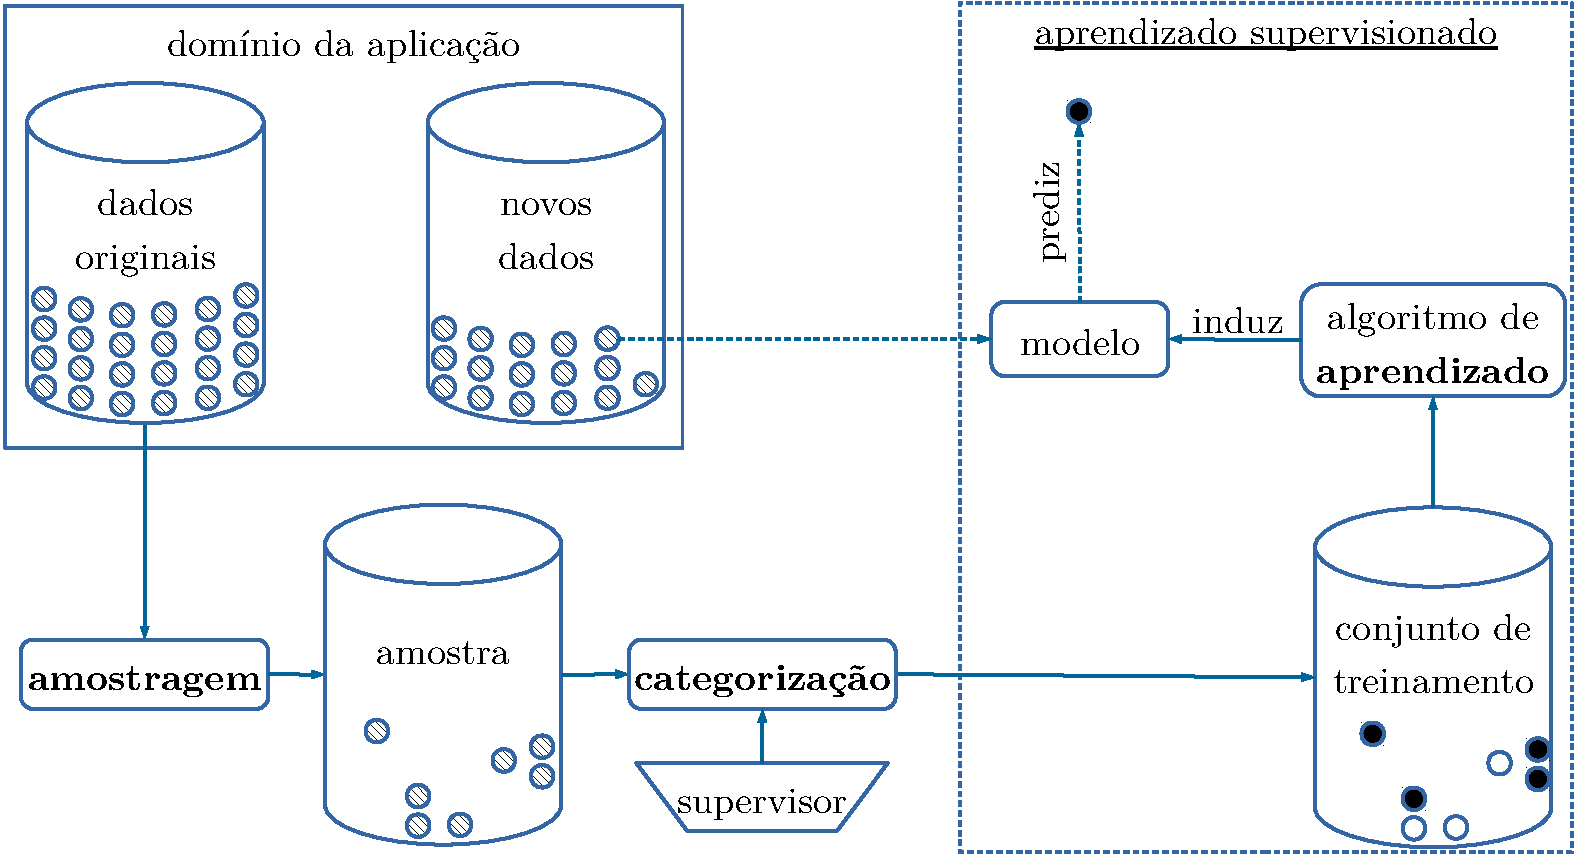
\includegraphics[scale=0.5]{apsup.pdf}
  \caption[Esquema de aprendizado supervisionado.]{Esquema de aprendizado supervisionado e componentes externos.}
  \label{aprsup}
\end{figure}
Uma amostra dos exemplos (ou todos) disponíveis no domínio do problema é classificada de acordo com as classes atribuídas por um supervisor.
O resultado é o conjunto de dados de treinamento para a geração de um \textit{modelo} de classificação.

\section{Motivação}\label{motiv}
Assumindo-se a disponibilidade de infraestrutura computacional, a necessidade de esforço humano pode se tornar o maior obstáculo para um projeto de aprendizado supervisionado ser bem sucedido.
Esse esforço pode ser necessário em pelo menos duas perspectivas de atuação que abrangem os passos em destaque na Figura \ref{aprsup}:
% sobre enumerações: http://www.portaleducacao.com.br/educacao/artigos/46190/pontos-fundamentais-da-gramatica-enumeracoes
\begin{itemize}
\item no projeto do sistema, tanto na escolha da forma de {amostragem} quanto na determinação do algoritmo de {aprendizado} mais adequado ao problema; e,
\item durante a {categorização} dos dados, normalmente realizada por um ou mais supervisores humanos.
\end{itemize}
No primeiro caso, um especialista em aprendizado de máquina toma decisões relacionadas à implementação do sistema.
No segundo caso, especialistas no domínio do problema fazem a \textit{rotulação}, ou seja, atribuem rótulos informando a classe de cada objeto de interesse.
As atividades realizadas nos dois momentos podem ter um custo elevado.

O custo de rotulação pode ser facilmente contabilizado pela quantidade de rótulos necessários para a construção do conjunto de treinamento.
Por outro lado, o custo das decisões do especialista é de estimação mais incerta, pois envolve o esforço despendido no processo de escolha e suas possíveis consequências.
Quanto menor a confiança desse especialista na escolha do processo de amostragem ou do algoritmo de aprendizado, maiores as chances da aplicação incorrer em custos adicionais ou prejuízo no desempenho preditivo futuro.
% 'tratar-se de' é sempre singular quando não é doença
Portanto, custo de rotulação e custo decorrente de inadequação do sistema à tarefa desejada são dois aspectos importantes - quando se deseja garantir a viabilidade financeira de uma aplicação.

Além da questão econômica, o desempenho do sistema também depende das decisões tomadas na fase de projeto.
Acurácia preditiva e tempo de processamento, por exemplo, são diretamente afetados pela escolha do algoritmo de aprendizado.
Ademais, a qualidade dos dados amostrados e o próprio viés da \textit{estratégia} de amostragem escolhida também influenciam diretamente no desempenho.
Logo, a definição do par \textit{estratégia-algoritmo} ideal para um dado problema tem um papel central no projeto de um sistema de aprendizado supervisionado como aquele exposto previamente na Figura \ref{aprsup}.
A necessidade de definição desse par motiva a realização de uma pesquisa que se aprofunde além da simples comparação de poucas estratégias de amostragem, com mais do que somente um algoritmo de aprendizado e mais do que uma dúzia de conjuntos de dados - como tem sido feito na literatura \cite{journals/corr/EvansAA14a,conf/emnlp/SettlesC08,journals/ml/ScheinU07,conf/ecml/KornerW06}.
% They have a restricted scope, such as focus on strategies for a particular 
% classification algorithm \cite{journals/ml/ScheinU07}, 
% specific tasks \cite{conf/emnlp/SettlesC08} or 
% a single family of strategies \cite{conf/ecml/KornerW06}.
% % http://arxiv.org/pdf/1408.1319.pdf
% In a recent comparison, active learning failed in \textit{more often than not}, according to
% \cite{journals/corr/EvansAA14a}.
% The authors used two strategies (Uncertainty Sampling and QBC) and
% four algorithms (Logistic Regression, Quadratic Discriminant Analysis,
% Random Forest and Support Vector Machines).
% Therefore, we believe more comprehensive studies and experiments attesting the active learning feasibility are necessary.

O cenário de \textit{aprendizado ativo} é explorado neste trabalho visando abordar o problema da redução do custo de rotulação (Seção \ref{aprendizado-ativo}).
Apenas os exemplos mais relevantes do conjunto de dados são escolhidos.
No cenário específico desta tese, que será detalhado na Seção \ref{desccen}, o conjunto de dados não rotulados é chamado \ing{reserva de exemplos}{pool}.
Nesse contexto, o conjunto de treinamento cresce enquanto houver \textit{orçamento} - seguindo o ciclo \mbox{\textit{consulta} \MVRightarrow\phantom{i}\textit{rotula} \MVRightarrow\phantom{i}\textit{induz}} 
apresentado na Figura \ref{apsupal}.
\begin{figure}
  \setlength{\unitlength}{1.0cm}
  \centering
    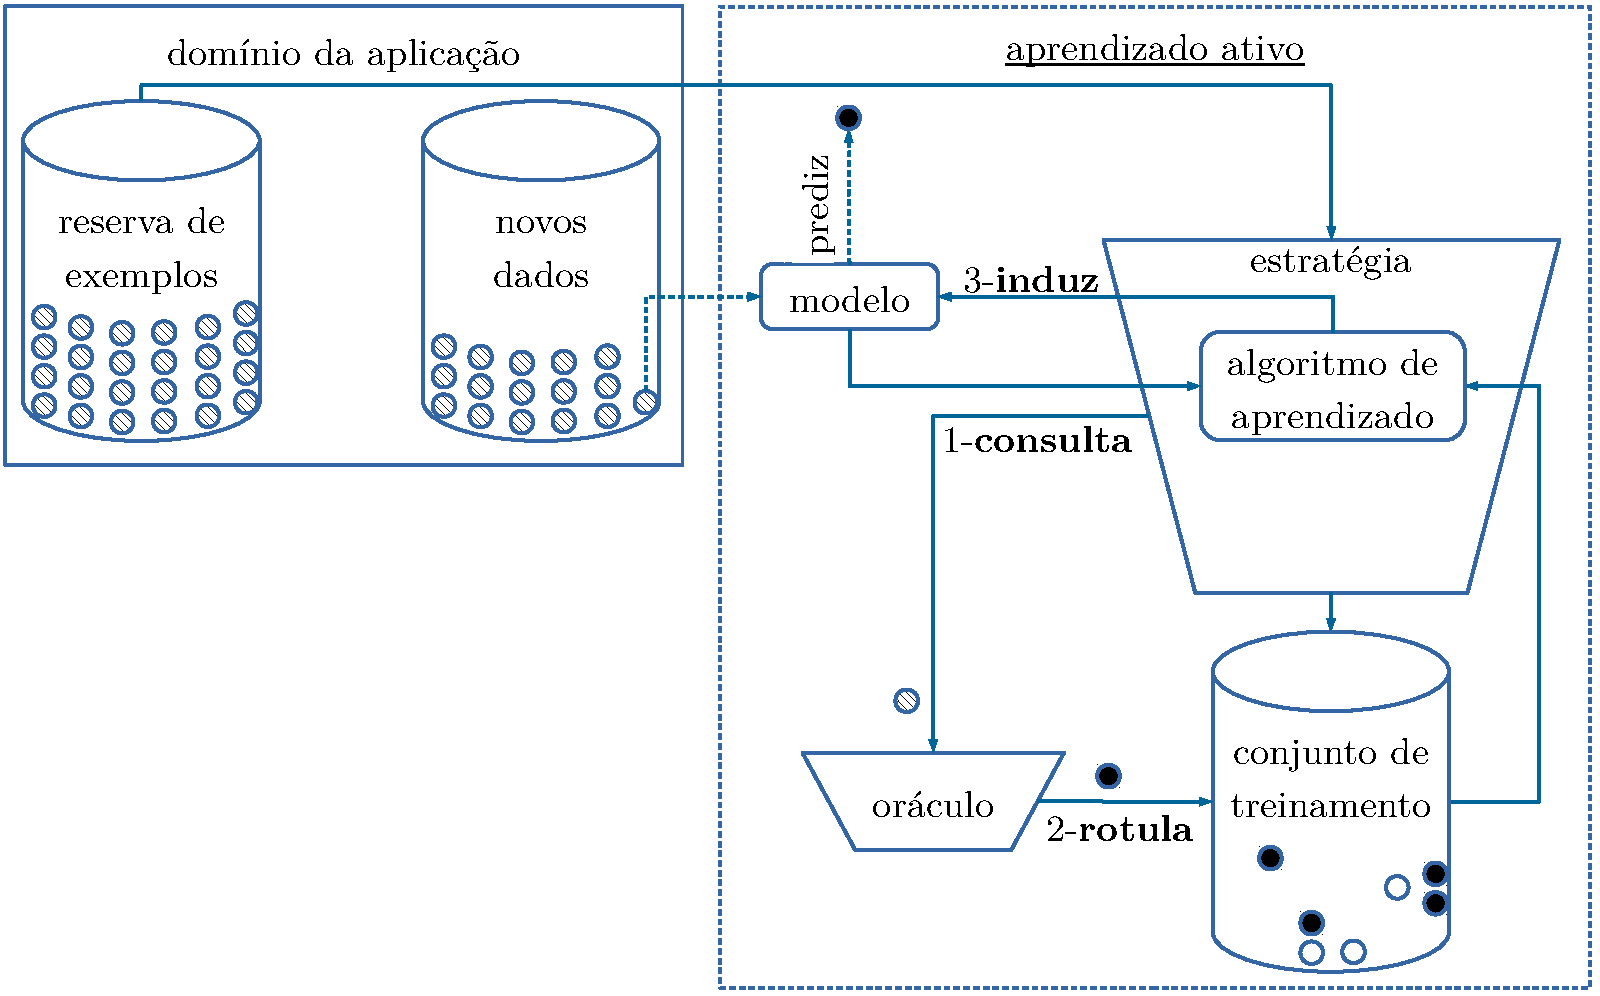
\includegraphics[scale=0.5]{apsupal.pdf}
  \caption{Esquema de aprendizado ativo.}
  \label{apsupal}
\end{figure}
Consequentemente, a administração do custo de rotulação passa a ser atribuição de uma estratégia de amostragem ativa.
Para fins experimentais, o orçamento indica o número de \textit{consultas} permitidas.

Finalmente, a questão da possível inadequação do algoritmo de aprendizado ao domínio do problema permanece em aberto.
Assim, a indução de um modelo adequado depende da escolha do par estratégia-algoritmo, ou apenas da estratégia, no caso excepcional em que tenha sido adotada uma estratégia sem \textit{aprendiz} (Capítulo \ref{contexto}).
Uma estratégia sem aprendiz é uma estratégia que não necessita de um algoritmo de aprendizado para realizar as consultas.
% , ou seja, que não recorra aos modelos gerados por algoritmos de aprendizado.
A motivação para a pesquisa em ambas componentes do par estratégia-algoritmo é dada nas seções \ref{ee} e \ref{ea}.

\subsection{Escolha da estratégia}\label{ee}
A existência de diversas estratégias na literatura de aprendizado ativo coloca o especialista em aprendizado de máquina diante de uma escolha para a qual não há um critério claro.
A principal dificuldade advém da impossibilidade de comparação dos desempenhos dessas diferentes abordagens 
% para um determinado conjunto de dados 
sem incorrer em custos de rotulação.
Isso se deve ao fato de que a qualidade das consultas é dada, em última instância, pela acurácia do modelo induzido.
Sendo a indução somente possível com a presença dos rótulos e esses são provenientes da interação estratégia-oráculo, tem-se um paradoxo:
a escolha da estratégia depende dos rótulos que, por sua vez, dependem da estratégia.

Na literatura da área, a escolha da estratégia a ser utilizada tem sido quase arbitrária, tendendo a se concentrar no uso da mais simples - a \textit{amostragem por incerteza}.
Essa preferência foi reportada numa competição de aprendizado ativo \cite{journals/jmlr/GuyonCDL11} - conforme ilustrado na Figura \ref{compet}.
% Nessa competição também prevaleceu a omissão de estratégias possivelmente mais efetivas (Capítulo \ref{experimentos}).
\begin{figure}
	\centering
	\includestandalone[mode=buildmissing]{images/barras}
	\caption[Frequência de uso de estratégias na competição de aprendizado ativo.]{Frequência de uso de estratégias na competição de aprendizado ativo - descritas na Seção \ref{secestrategias}.
	Alguns participantes adotaram mais de uma estratégia.
	\textit{Adaptado de \citeonline{journals/jmlr/GuyonCDL11}.}}
	\label{compet}
\end{figure}
% challenge:
% global_score = (ALC-Arand)/(Amax-Arand)       Amax = 1
% semi-supervised learning is needed to achieve good performance in the first part of the learning curve
% (usar ou não semisupervised é um problema à parte, que faz parter do learner, não da estratégia; classificadores semisupervisionados são melhores, mas não é isso que se está avaliando quando se comparam estratégias; ensembles, feature selection e SMOTE também ajudam e nem por isso precisam ser empregados na comparação de estratégias)
Em consonância com esse panorama está a ausência de estudos comparativos abrangentes que possam guiar o especialista na definição da estratégia de consulta a ser empregada - até onde o conhecimento do autor desta tese permite dizer.
Consequentemente, a maneira ideal de redução do custo de rotulação ainda é um problema em aberto.

\subsection{Escolha do algoritmo}\label{ea}
A questão da escolha do algoritmo de aprendizado para a indução de modelos de classificação é análoga à questão da escolha da estratégia.
A escolha do algoritmo é definida neste texto da seguinte forma: seleção \textit{manual} - baseada em experiência pessoal de experimentos anteriores do especialista; ou, seleção \textit{automática} - baseada em sistemas de recomendação, como o \textit{meta-aprendizado} (Apêndice \ref{apmeta}).
% 'meta-aprendizado' é pouco mencionado aqui. Ele só vai ser abreviado depois que for definido no capítulo correspondente, para evitar confusão aqui com outras siglas.

Usualmente, ambas abordagens (manual e automática) empregam validação cruzada durante a comparação de algoritmos candidatos \cite{conf/pakdd/BouckaertF04,books/daglib/0022052}.
Isso as torna mais aplicáveis ao cenário em que o conjunto de treinamento já esteja construído.
Entretanto, no cenário de aprendizado ativo, a rotulação é um processo em andamento, assim como seu conjunto de treinamento resultante.
Tal característica impede que o especialista disponha da importante fonte de informação que um conjunto de treinamento completo poderia representar.
Reduz-se, assim, a quantidade de informações disponíveis para decisões bem fundamentadas.
Logo, além da escolha da estratégia ser incerta pela falta de critérios, conforme visto na Seção \ref{ee}, a escolha do algoritmo mais adequado para o papel de aprendiz também carece de melhores fundamentos.

\section{Hipóteses}\label{hipoteses}
O teorema conhecido como \sigla{NFL}{\textit{No Free Lunch}} permite afirmar que nenhum algoritmo de aprendizado pode ser o mais adequado para todos os domínios \cite{conf/icml/Schaffer94}.
A mesma afirmação é válida para algoritmos de otimização \cite{journals/tec/DolpertM97} e, consequentemente, válida para estratégias de amostragem ativa.
Assim, é garantida a existência da questão da escolha no presente cenário do ponto de vista teórico.
A razão de uma estratégia poder ser entendida como um procedimento de otimização é ela consistir na busca pela melhor sequência de exemplos dentro das possibilidades que a reserva de exemplos e o orçamento permitem.
Dessa forma, é possível definir o contexto para as hipóteses desta tese:
\textit{cada estratégia tem um viés de amostragem, normalmente dependente de um viés de aprendizado, que favorece determinados domínios de problemas e prejudica outros}.
% - analogamente ao viés de aprendizado de um algoritmo de classificação passiva. 
Diante desse cenário, e considerando a motivação apresentada previamente
na Seção \ref{motiv}, duas hipóteses foram formuladas.
A Hipótese I corresponde à principal tese defendida neste trabalho:
% enumeração seguida de ponto final pede inicial maiúscula

\noindent\fbox{\parbox{.98\textwidth}{
É possível explorar relações entre conjuntos de dados e 
\textit{algoritmos de aprendizado, estratégias de aprendizado ativo ou pares de ambos}, de maneira que seja possível escolher abordagens para essas duas componentes que resultem num melhor desempenho preditivo que uma escolha arbitrária.}}\\

A Hipótese II, secundária, supõe que \textit{a presença ou tipo do viés de aprendizado podem ser controlados durante o processo de rotulação, aumentando o desempenho preditivo}.
% a concordância entre o verbo e o sujeito depende do valor da conjunção 'ou' (inclusivo ou exclusivo) 

A Seção \ref{intropropostas} contém a proposta de investigação das hipóteses.

\section{Proposta}\label{intropropostas}
A proposta desta tese é a investigação de alternativas para facilitar a escolha da estratégia de amostragem e/ou seu correspondente algoritmo de aprendizado mais adequados para um conjunto de dados.
Uma particularidade do cenário de aprendizado ativo é que o subconjunto inicial de exemplos rotulados é vazio ou pequeno demais para escolhas apropriadas.
% 'alternativas' inclui análise de nichos, HTU e culmina em MTL;
Assim, o resultado esperado da investigação é que a escolha da estratégia, do algoritmo ou do par estratégia-algoritmo possa ser realizada de uma maneira mais objetiva que a convencional, induzindo modelos com melhor acurácia preditiva para um dado orçamento.
% Isso será atestado vencendo a escolha arbitrária (majoritário).

% \subsection{Investigação}\label{invest}
A investigação concentra-se nos seguintes objetivos, em ordem decrescente do grau de participação requerida do especialista que hipoteticamente usufruiria dos resultados:
\begin{itemize}
   \item identificação de nichos de problemas onde a utilização de certas estratégias seja adequada - teste qualitativo da Hipótese I;
   \item desenvolvimento de uma estratégia capaz de suprimir a influência do algoritmo de aprendizado na fase de rotulação, quando seu uso for prejudicial - teste da Hipótese II; e,
   \item teste inicial de uma estratégia que poderia ser chamada \textit{aprendizado meta-ativo}\footnote{Note-se a distinção entre \textit{aprendizado meta-ativo} e \textit{meta-aprendizado ativo} \cite{conf/ijcnn/SousaPSL13} explanada na Seção \ref{sec:ama}.} (meta-aprendizado aplicado a aprendizado ativo) capaz de escolher (e trocar) o algoritmo antes de (e durante) o aprendizado - teste quantitativo das Hipóteses I e II. 
\end{itemize}
Os meios escolhidos para atingir essas metas são: revisão bibliográfica; implementação própria de \textit{software} e reuso de bibliotecas de terceiros; aplicação dos métodos propostos em problemas relevantes; comparação com referências importantes da área; e, avaliação e validação dos resultados obtidos.

As principais contribuições e resultados decorrentes da implementação da proposta são apresentados na Seção \ref{contribuicao}.

\section{Contribuição}\label{contribuicao}
As contribuições deste trabalho são originais até onde o conhecimento do autor permite dizer.
Os resultados obtidos e publicações resultantes são listados nas seções seguintes.

\subsection{Resultados}\label{introres}
Este trabalho foi baseado em experimentos que simulassem situações representativas da realidade - naturalmente, dentro das limitações próprias de qualquer avaliação empírica, como a definição da coleção de conjuntos de dados, do conjunto de estratégias de aprendizado ativo e do conjunto de algoritmos de aprendizado.
Os resultados obtidos, dentro do arcabouço experimental adotado, são apresentados a seguir.
\begin{itemize}
	\item A estratégia HTU (Seção \ref{newhtu}), proposta para controle da atuação do aprendiz e, similarmente, ATU (Seção \ref{newag}), proposta para avaliar o efeito da ausência de aprendiz, mostraram-se, em vários aspectos, as de menor risco para o orçamento dentre as abordagens comparadas - sem incorrer em redução na acurácia preditiva.

	\item As possíveis adequações e inadequações entre estratégias, algoritmos de aprendizado e conjuntos de dados foram ilustradas por meio de árvores de decisão e curvas de aprendizado, de forma que foi possível identificar a influência preponderante do algoritmo no desempenho preditivo ao longo do aprendizado.

	\item A escolha automática do algoritmo de aprendizado requer investigações mais extensivas. Na presença, dentro da coleção, de mais de conjunto de dados de cada domínio, tal escolha automática superou a escolha arbitrária e a referência da área (Apêndice \ref{apmeta}).
	
	\item Outras modalidades de recomendação automática também foram experimentadas e se mostraram mais desafiadoras: recomendação de estratégias e recomendação de pares estratégia-algoritmo.
	
	\item Algumas modalidades de recomendação foram percebidas como desafios sem indícios de viabilidade: recomendação de métricas de distância para estratégias baseadas em densidade e recomendação sobre adotar ou não aprendizado ativo.
	
	\item As características mais relevantes dos conjuntos de dados para a recomendação automática foram organizadas visualmente numa estrutura de árvore de decisão e brevemente discutidas.
\end{itemize}

Em síntese, os experimentos mostraram que é possível obter modelos com melhor desempenho preditivo no cenário de aprendizado ativo, caso alguma das abordagens propostas, ou uma combinação delas, seja adotada: ATU, HTU e, num cenário mais restrito e dependente de maiores investigações quanto à sua real viabilidade, aprendiz meta-ativo.

\subsection{Publicações}\label{intropub}
As contribuições são diretamente ligadas às hipóteses previamente apresentadas e são enumeradas como segue, juntamente com as publicações decorrentes.
\begin{enumerate}
	\item \label{item1} Demonstração da influência determinante do algoritmo de aprendizado adotado como aprendiz - submetido por \citeonline{revistainvestigation}.
	\item \label{item2} Experimentação inicial de uma nova abordagem para aprendizado ativo,  chamada \textit{aprendizado meta-ativo}, cujo objetivo é buscar o algoritmo com o melhor viés para um dado conjunto de dados - submetido por \citeonline{revistametaartigo}.
	\item Experimentação da mesma abordagem do Item \ref{item2} é em outras modalidades de recomendação como: estratégia e pares estratégia-algoritmo - artigo em processo de escrita.
	\item \label{item4} Uma estratégia baseada na inibição do aprendiz enquanto ele for potencialmente prejudicial - publicado por \citeonline{bracis15}.
\end{enumerate}
Publicações referentes a contribuições metodológicas ou visando contribuir com a organização da área de aprendizado ativo são enumeradas a seguir.
\begin{enumerate}[resume]
   \item \label{item5} Comparação descritiva e experimental de estratégias da literatura utilizando 28 conjuntos de dados e algoritmos de aprendizado com vieses diversos - publicado por \citeonline{conf/hais/SantosC14}.
   \item Adaptação de estratégias para o cenário multiclasse - idem ao Item \ref{item5}.
   \item Comparação e adaptação de estratégias utilizando um algoritmo ainda pouco explorado no cenário de aprendizado ativo: as redes neurais com pesos aleatórios \cite{schmidt1992feedforward} - publicado por \citeonline{santos2014viabilidade}.
   \item Proposta metodológica das \textit{curvas de ranqueamento\footnote{Apesar do vocábulo estrangeiro \textit{ranking} constar no léxico contemporâneo da língua portuguesa \cite{academia2004vocabulario}, optou-se aqui pela grafia \textit{ranqueamento} já presente na literatura brasileira da área \cite{colares2005processo}, pois seu radical permite outras possibilidades não contempladas pelo léxico, como \textit{ranqueado} e \textit{ranqueável}.}}, que contornam a dificuldade de apresentação das curvas de aprendizado obtidas em experimentos com 39 conjuntos de dados - idem aos itens \ref{item1} e \ref{item4}.
\end{enumerate}

Adicionalmente, os seguintes sistemas de \textit{software} foram desenvolvidos e disponibilizados publicamente.
\begin{enumerate}[resume]
  \item Biblioteca de encapsulamento de algoritmos de classificação \cite{doi/ml}.
  \item Biblioteca de estratégias de amostragem ativa e ambiente experimental \cite{doi/al}.
\end{enumerate}
Finalmente, dois artigos resultaram de colaboração com outros grupos de pesquisa, envolvendo extração de atributos de séries financeiras \cite{conf/dexa/BedoSKT13} e seleção de métodos de extração de atributos \cite{Bedo2015jdi}.

\section{Estrutura do documento}\label{estrutura}
O contexto da pesquisa e a notação matemática, incluindo a terminologia adotada, são apresentados no Capítulo \ref{contexto}.
O capítulo também contém uma revisão da literatura fundamental para esta tese: aprendizado de máquina e aprendizado ativo.
No Capítulo \ref{propostas}, são apresentadas as abordagens propostas ou adaptadas: ATU, HTU, SGmulti e a possibilidade experimentada de aprendizado meta-ativo.
O Capítulo \ref{metodologia} contém a descrição do cenário escolhido; a enumeração das estratégias, algoritmos e conjuntos de dados adotados; e, a apresentação dos métodos de avaliação comuns a todos os experimentos realizados.
A proposta metodológica chamada \textit{curvas de ranqueamento} é introduzida nesse capítulo.

A avaliação empírica e seus resultados associados são apresentados
no Capítulo \ref{experimentos}.
Por fim, no Capítulo \ref{conclusao}, é feita uma análise geral das metas atingidas, contribuições, dificuldades e limitações da pesquisa realizada.
Possíveis desdobramentos futuros são delineados ao final do capítulo.

Alguns conteúdos foram registrados em apêndices e anexos para brevidade do corpo principal do texto: revisão sobre meta-aprendizado (Apêndice \ref{apmeta}), ferramentas utilizadas (Apêndice \ref{apfer}), descrição da coleção de conjuntos de dados adotada (Apêndice \ref{apdatasets}), atividades complementares  (Anexo \ref{anc}) e resultados detalhados (Anexo \ref{anresdet}).
Os apêndices \ref{apexpcom} e \ref{apflu} contêm experimentos e resultados adicionais sobre aprendizes ativos baseados em comitês e o efeito da similaridade entre conjuntos de dados, respectivamente.

\chapter{Contexto} \label{contexto}
\epigraph{
\textit{\ldots no matter how many instances of white swans we may have observed, this does not justify the conclusion that \emph{all} swans are white.
}}{Karl Popper\footnotemark[1]}
\setcounter{footnote}{1}
\footnotetext[1]{\aspas{\ldots não importa quantos exemplos de cisne branco tenhamos observado, isso não justifica a conclusão de que \emph{todos} os cisnes sejam brancos.} - \citeonline{popper1959survey}, sobre o problema da indução na ciência e a necessidade do princípio da falseabilidade.} 
A pesquisa realizada exige a apresentação dos temas pertinentes e as definições adotadas no presente documento, incluindo notação e terminologia.
A contextualização se inicia na Seção \ref{cla}, onde a tarefa de classificação, no contexto de aprendizado de máquina, é apresentada em termos gerais.
O assunto central desta tese, que engloba o aprendizado ativo e suas principais estratégias, é introduzido nas seções \ref{aprendizado-ativo} e \ref{secestrategias}.
Finalmente, na Seção \ref{contcons}, são feitas considerações a respeito dos temas abordados e uma comparação objetiva entre as estratégias.

\section{Classificação}\label{cla}
% Algumas habilidades humanas vêm claramente programadas geneticamente,
% como a amamentação \cite{gunther1955instinct}.
% Outras são apenas a execução de uma lista de passos memorizados, como o trabalho efetuado numa determinada posição de uma linha de montagem industrial.
% Apesar do amplo escopo de ação desses dois tipos de conhecimento (genético e memorizado), existem ainda outras habilidades adquiríveis sem que seja necessária uma programação prévia.
% O reconhecimento de novos objetos, por exemplo, é uma tarefa aprendida por humanos em que é difícil depreender os algoritmos nos quais ela se baseia.
A atividade de identificação da categoria de um determinado objeto de interesse é chamada \textit{classificação}.
Ela é a tarefa que pode se beneficiar mais amplamente dos resultados da presente pesquisa.
Seus principais conceitos são apresentados nas seções seguintes juntamente com a forma de representação adotada neste texto.
% \ref{defmod}, \ref{defcla}, \ref{defatr} e \ref{defpro}.
Essa exposição tem o objetivo de facilitar consultas posteriores sobre terminologia durante a leitura dos demais capítulos.
As escolhas de alguns símbolos são baseadas no livro de \citeonline{series/synthesis/2012Settles}.

\subsection{Modelo}\label{defmod}
\simbolo{\theta}{modelo induzido}
\simbolo{\theta_{\mathcal{L}'}}{modelo induzido com exemplos do conjunto $\mathcal{L}'$}
\simbolo{\Theta}{conjunto de modelos possíveis}
O aprendizado de um determinado conceito pode ser visto como uma busca dentro do espaço de hipóteses representado pelo conjunto $\Theta$ de modelos de representação possíveis.
Assim, a tarefa de classificação induz um modelo $\theta \in \Theta$ baseado num conjunto de dados de treinamento, cujos rótulos foram previamente fornecidos por um especialista no domínio do problema (Seção \ref{motiv}).
Os algoritmos de aprendizado são considerados determinísticos, por simplicidade.
% Na notação adotada nesta tese, o subscrito $(t), t \in \mathbb{N}$, representa a apresentação de cada novo exemplo do conjunto de treinamento e, consequentemente, o tamanho deste no momento.
% O uso de parênteses visa diferenciá-lo mais claramente do subscrito convencional de vetores que indica o valor para uma dada posição, por exemplo, quando $\bm{v} = (4,3,2,1)$, $v_3=2$; ao passo que $\bm{v}_{(t)}$ representaria um vetor (todos os valores) no momento $t$.
% Esse subscrito somente é usado quando o contexto exige situar o aprendizado no tempo, na medida em que a quantidade de exemplos aumenta um a um.

% A área que engloba algoritmos capazes de aprender, não apenas para classificação, é chamada \textit{aprendizado de máquina} (aprendizado).
% Uma de suas metas é a construção de modelos sem programação explícita \cite{journals/cacm/Valiant84}.
% Diversas tarefas como bioinformática \cite{journals/bmcbi/WangLLXHXL14},
% visão computacional \cite{conf/nips/KrizhevskySH12} e
% recomendação de conteúdo \cite{reference/rsh/RicciRS11}
% têm sido bem sucedidas atualmente.
Antes da construção de cada modelo $\theta$, é desejável saber qual parte dos dados é relevante.
Esse é um problema em aberto que pode ser entendido como uma busca pela melhor maneira de se amostrarem os dados.
A motivação para essa busca pode frequentemente advir da intratabilidade de um excesso de dados ou da escassez de recursos para manutenção de um especialista no papel de supervisor.
Ambos os casos podem se beneficiar do tipo de aprendizado denominado \textit{ativo}; que será apresentado na Seção \ref{aprendizado-ativo}.

\subsection{Classe}\label{defcla}
% \simbolo{c \in C}{classe e respectivo conjunto}
\simbolo{y \in Y}{classe e conjunto de classes possíveis}
Neste texto, o termo \textit{classificador} refere-se ao modelo $\theta$ mais recente induzido pelo algoritmo de aprendizado, quando o objetivo é a predição de classes - diferentemente de quando o objetivo é a estimação de probabilidades, por exemplo, cujos valores de retorno são contínuos.
A classe $y$ de um exemplo é um dos elementos do limitado conjunto $Y$ de classes de um dado problema.
% vetor binário $\bm{y}$ pertencente ao conjunto de classes possíveis $Y$ formalmente definido pela Equação \ref{ydef}.
% \begin{equation}\label{ydef}
%  Y = \{\bm{y} \mid y_o=1, y_p=0 \forall o \neq p, 1 \leq p \leq |C|\}
% \end{equation}
% Essa representação binária, por exemplo, $\Y=\{(0,0,1),(0,1,0),(1,0,0)\}$,
% corresponde à representação \ing{um-de-n}{one-hot encoding} \cite{Harris:2007:DDC}.
% O vetor $\bm{y}=(0,1,0)$ é um exemplo de representação de classe,
% chamado no texto apenas de \textit{classe} por conveniência.

\subsection{Atributos}\label{defatr}
\simbolo{\bm{x} \in X}{tupla/vetor de atributos e conjunto de tuplas válidas}
\simbolo{\phi}{função de indução de modelos}
\simbolo{A \in \mathcal{A}}{conjunto de valores válidos do atributo $A$ e conjunto de atributos existentes}
\simbolo{\mathcal{L}}{conjunto de exemplos rotulados}
\simbolo{\mathcal{\bar{L}}}{conjunto de exemplos rotulados ponderados}
\simbolo{\mathcal{U}}{reserva de exemplos}
\simbolo{V_i}{sequência de valores ocorridos para $x_i, \bm{x} \in \mathcal{U}$}
Um exemplo não rotulado é dado por uma tupla de \textit{atributos}\footnote{Neste texto, os \textit{atributos} de um exemplo não incluem a classe do exemplo, exceto quando explicitado como \textit{atributo alvo}.} $\bm{x}$ pertencente ao conjunto $X$ de tuplas válidas - ou \textit{vetores} válidos, se o contexto exigir e assumindo uma binarização prévia dos atributos nominais, caso existam.
Dessa forma, a representação de um exemplo rotulado é um par
%  \ano{dupla/tupla?}
$\langle \bm{x}, y \rangle \in X\times Y$.
Dado um subconjunto contido em $X \times Y$, cada algoritmo de aprendizado tem sua própria 
função de indução de modelos\footnote{A notação $2^B$ representa o conjunto de todos os subconjuntos de $B$ - chamado \textit{potência} ou \textit{de partes} \cite{devlin2012joy}.}
$\phi\colon 2^{X\times Y} \rightarrow \Theta$.

% No contexto teórico uso a palavra 'problema' para restringir o conceito à matemática da coisa. É também importante para a definição formal do 'problema de aprendizado ativo' mais à frente.
Cada atributo é representado por um conjunto de valores $A \in \mathcal{A}$, onde $\mathcal{A}$ é o conjunto de atributos do problema.
Este é dado pela Equação \ref{eqa}, onde $\dime{\bm{x}'}$ indica a dimensão de qualquer $\bm{x}'\in X$.
\begin{equation}\label{eqa}
\mathcal{A} = \{\{x_i \mid \bm{x} \in X\} 
\mid
1 \leq i \leq \dime{\bm{x}'}\}
\end{equation}
Assim, cada conjunto de valores $A$ contém os valores que cada atributo de $\bm{x}$ pode assumir.
Por exemplo, sendo o primeiro atributo $A=\{\textit{alto},\textit{medio},\textit{baixo}\}$,
é possível que $x_1=medio$; ou, sendo o segundo atributo $A' = \mathbb{R}$, $x_2=3,7$.
Diferentemente, $V_i$ é a 
sequência - ou vetor, dependendo do contexto - de todos os valores ocorridos para o atributo correspondente à componente $x_i$ de todos os exemplos da reserva $\mathcal{U} \subset X$ - conforme Equação \ref{eqv}.
\begin{equation}\label{eqv}
   V_i = \langle x_i \mid \bm{x} \in \mathcal{U} \rangle
\end{equation}
A reserva de exemplos ($\mathcal{U}$) consiste no conjunto de exemplos não rotulados disponíveis numa dada aplicação.
O tipo do atributo é dado pela função $\nom\colon \mathcal{A}\rightarrow\{0,1\}$ que retorna $1$ para atributos nominais e $0$ para atributos numéricos.
O conjunto de exemplos rotulados é representado por $\mathcal{L}$.
Eventualmente, nas situações em que seja necessário atribuir pesos aos exemplos, cada exemplo é representado por uma tripla $\langle \bm{x}, y, w \rangle, 0 \leq w \leq 1$.
Nesse caso, o \textit{conjunto rotulado de exemplos ponderados} é dado pelo símbolo $\mathcal{\bar{L}}$.

\simbolo{\mathcal{F}}{espaço de atributos transformado}
O termo \textit{espaço de atributos} representa um espaço em $\mathbb{R}^{|\mathcal{A}|}$ onde cada exemplo pode ser situado.
Essa definição pressupõe a binarização de atributos nominais, quando necessário.
Ela difere do \textit{espaço de parâmetros} $\mathcal{F}$ que é um espaço de atributos transformado, cujo exemplo típico de coordenadas é o conjunto de pesos de uma rede neural \cite{haykin2004comprehensive}.

\subsection{Valores de retorno}\label{defpro}
\simbolo{P_{\theta} (\bm{y}\mid\bm{x})}{probabilidade de ocorrência da classe $y$ dado $\bm{x}$ - segundo o modelo $\theta$}
\simbolo{\bm{P}_{\sim\theta} (\bm{x})}{vetor com a distribuição de probabilidades para $\bm{x}$ - segundo o modelo $\theta$}
\simbolo{\hat{y}_{\theta}(\bm{x})}{classe mais provável do exemplo $\bm{x}$ de acordo com modelo $\theta$}
\simbolo{\info(\bm{x})}{medida de informatividade de $\bm{x}$}
\simbolo{f_i(\bm{x})}{função preditiva da classe $y_i$}
\simbolo{g}{função sigmoide logística}
Dado um exemplo $\bm{x}$, e supondo que o modelo $\theta$ permita a estimação da probabilidade $P_{\theta}$ de $\bm{x}$ ter a classe $y$,
a classe mais provável $\hat{y}_\theta$ é obtida pela Equação \ref{p}.
\begin{equation}\label{p}
  \hat{y}_\theta(\bm{x}) = \argmax_{y} P_{\theta} (y\mid\bm{x})
\end{equation}
$P_{\theta}$ é a base de grande parte das medidas de \textit{informatividade} $\info(\bm{x})$ empregadas pelas estratégias.
Entretanto, modelos não probabilísticos podem retornar valores numéricos que não representam uma distribuição de probabilidades.
Esses valores são resultado de uma função preditiva $f_y(\bm{x})$:
valores próximos de $1$ indicam pertinência à classe $y$.
Classificadores cujos modelos retornam valores fora do intervalo $[0;1]$ podem fazer uso da função sigmoide logística exibida na Equação \ref{eqsig} para cada classe $y$ \cite{von2006crc}.
\begin{equation}\label{eqsig}
   g_y(\bm{x})=\frac{1}{1+e^{-f_y(\bm{x})}}
\end{equation}

$\bm{P}_{\sim\theta}$ representa a sequência com a distribuição de probabilidade das classes para um dado exemplo $\bm{x}$.
Por exemplo, $\bm{P}_{\sim\theta}(\bm{x})=\langle 0; 0,5; 0,4; 0,1\rangle, |Y|=4$.

\simbolo{R_{\theta}(\mathcal{N})}{matriz de confusão para o conjunto de teste $\mathcal{N}$ de acordo com o modelo $\theta$}
\simbolo{r(R_{\theta})}{acurácia convencional para a matriz de confusão $R_{\theta}$}
\simbolo{\bm{e}(R_{\theta})}{vetor de ocorrências esperadas na matriz de confusão $R_{\theta}$}
\simbolo{\bm{p}(R_{\theta})}{vetor de ocorrências preditas na matriz de confusão $R_{\theta}$}
\simbolo{o(\bm{x})}{função/oráculo que revela o rótulo do exemplo $\bm{x}$}
A matriz de confusão $R_{\theta}\colon 2^{X \times Y} \rightarrow \mathbb{R}^{|Y|\times|Y|}$ possibilita o cálculo de importantes medidas de desempenho \cite{stehman1997selecting}.
Ela representa uma tabela de frequências de classes preditas para cada classe esperada.
Supondo um conjunto de teste $\mathcal{N}$, a matriz de confusão seria denotada por  $R_{\theta}(\mathcal{N})$, porém, dependendo do contexto, o parâmetro $\theta$ e o conjunto de teste $\mathcal{N}$ podem ser omitidos.
A notação para a acurácia convencional é representada, neste texto, por $r(R_{\theta})$.
Os vetores de ocorrências esperadas e preditas são dados, respectivamente, por $\bm{e}(R_{\theta})$ e $\bm{p}(R_{\theta})$.
A verdadeira classe de um exemplo é revelada pela função oráculo $o\colon X \rightarrow Y$.

\subsection{Validação}
\simbolo{\mathcal{P}_i(\mathcal{L})}{partição $i$ do conjunto $\mathcal{L}$}
\simbolo{k}{número de partições da validação cruzada}
\simbolo{\kappa(S)}{índice kappa multiclasse para a matriz de confusão S}
\simbolo{\mathcal{M}}{conjunto de exemplos de treinamento ou reserva para aprendizado ativo}
\simbolo{\mathcal{N}}{conjunto de exemplos separados para teste}
\simbolo{S}{matriz de confusão cumulativa}
Para a aplicação de validação cruzada (Capítulo \ref{metodologia}), $\mathcal{L}$ é dividido em $k$ partições.
Assume-se, por simplicidade, que $|\mathcal{L}|$ é divisível por $k$.
Assim, $\mathcal{P}_i(\mathcal{L})$ representa a partição de índice $i$ conforme condições \ref{c1}, \ref{c2}, \ref{c3} e \ref{c4}.
\begin{equation}\label{c1}
  \bigcup\limits_{1 \leq i \leq k} \mathcal{P}_i(\mathcal{L}) = \mathcal{L}
\end{equation}
\begin{equation}\label{c2}
  \mathcal{P}_i(\mathcal{L}) \neq \varnothing, 1 \leq i \leq k
\end{equation}
\begin{equation}\label{c3}
   |\mathcal{P}(\mathcal{L})| = \frac{|\mathcal{L}|}{k}
\end{equation}
\begin{equation}\label{c4}
  \mathcal{P}_i(\mathcal{L}) \cap \mathcal{P}_j(\mathcal{L}) \neq \varnothing \Rightarrow \mathcal{P}_i(\mathcal{L})=\mathcal{P}_j(\mathcal{L})
\end{equation}
O Algoritmo \ref{algvc} descreve o procedimento de validação cruzada para a medida de desempenho adotada nesta tese (Seção \ref{newhtu}).
\begin{algoritmo}
\caption{Validação cruzada.}
\label{algvc}
\small
\Entrada{
 \\ $k$ - número de partições da validação cruzada
 \\ $\phi: 2^{X\times Y} \to \Theta$ - função indutora (algoritmo de aprendizado ou estratégia de amostragem ativa)
 \\ $\mathcal{L}$  - conjunto de dados rotulados
}
\Resultado{
 \\ $\kappa$ - índice kappa (Seção \ref{medidas})
}
  \algalg{\vc{$k$, $\phi$, $\mathcal{L}$}} {
  $S \leftarrow 0_{|Y|,|Y|}$ \come{matriz de confusão cumulativa} \\
  \ForEach {$i, 1 \leq i \leq k$} {
      $\mathcal{M}=\bigcup\limits_{j\neq i}\mathcal{P}_j(\mathcal{L})$ \come{exemplos disponíveis}\\
      $\mathcal{N}=\mathcal{P}_i(\mathcal{L})$ \come{exemplos reservados para teste}\\
      $\theta = \phi(\mathcal{M})$ \\
      $S \leftarrow S + R_\theta(\mathcal{N})$
    }
    \Return $\kappa(S)$
  }
\end{algoritmo}

  






% % % % % % % % % % % % % % % % % % % % % % % % % % % % % % % % % % % % % % % % % % % % % % % 
 % % % % % % % % % % % % % % % % % % % % % % % % % % % % % % % % % % % % % % % % % % % % % % 
%  verificar se tudo isso aparece nas tabelas de simbolos e siglas
% 
% exemplo a ser consultado $\hat{\bm{x}}$
% 
% $M(\bm{x})$ margem
% 
% $E(\bm{x})$ entropia
% 
% $JS$
% 
%  número de membros $M$
%  
%  $S$ e $G$
% de todas as hipóteses possíveis,
% denominadas $h_S \in S$ e $h_G \in G$, respectivamente.
% 
% modelos específico
% $\theta_S^{(m)}$ e geral $\theta_G$
% 
% classe mais provável,
% representada pelo vetor preditivo $\bm{y}'$
% 
% $O$ é a função objetivo
% 
% Rnd
% 
% Unc
% 
% Mar
% 
% SVMsim
% 
% SVMbal
% 
% KFF
% 
% QBC
% 
% QBCRFw
% 
% SG-network
% 
% SGmulti/CAL
% 
% EER
% 
% Inf
% 
% sim
% 
% d


%   \begin{equation}
% h\colon \mathcal{D} \rightarrow \{-,+\}
% \end{equation}

\subsection{Algoritmos de aprendizado}\label{algs}
Os algoritmos de aprendizado relevantes para esta tese serão mencionados no Capítulo \ref{metodologia} juntamente com os valores adotados para seus parâmetros.

\section{Aprendizado ativo} \label{aprendizado-ativo}
\input tex/active-learning

\section{Considerações}\label{contcons}
Neste capítulo, os assuntos que contextualizam esta tese foram revisados:
classificação, aprendizado ativo e suas estratégias.
Outro assunto relevante por integrar a proposta de \textit{aprendizado meta-ativo} é o \textit{meta-aprendizado}, cuja revisão bibliográfica é resumida no Apêndice \ref{apmeta}.

A literatura de aprendizado ativo é vasta.
Logo, a revisão bibliográfica das estratégias é invariavelmente incompleta.
Porém, a variedade de abordagens contidas na presente revisão é suficiente para a finalidade de teste das hipóteses desta tese.
Essa diversidade proporcionou diferentes níveis de adequação entre estratégias, algoritmos de aprendizado e conjuntos de dados (conforme será apresentado no Capítulo \ref{experimentos}).

Por fim, o Quadro \ref{stratsparcial} contém uma síntese das estratégias e suas características, conforme descrito a seguir.
\begin{itemize}
   \item Forma de \textbf{busca}: define se a consulta favorece abrangência ou eficiência; se ambas as metas são balanceadas de acordo com um critério simples ou combinadas de maneira alternada; e, se cada consulta se restringe apenas a parte dos dados.
   \item \textbf{Aprendiz}: indica se a estratégia tem ou não aprendiz e, caso tenha, se o algoritmo de aprendizado é fixo, específico da estratégia.
   \item \textbf{Dependência} entre consultas: define se o oráculo é necessário durante a amostragem ou pode ser consultado quando todos os exemplos relevantes já tiverem sido definidos pela estratégia.
   \item Ordem de \textbf{complexidade}: custo computacional considerando a quantidade de exemplos a aprender por consulta.
\end{itemize}


\begin{quadro}
\caption[Características de cada estratégia.]{Características de cada estratégia.}
\label{stratsparcial}
\centering
\begin{threeparttable}
\begin{tabular}{|l|p{3cm}|p{2cm}|l|p{3.2cm}|}
\hline
\textbf{Estratégia}		& \textbf{Busca}		&\textbf{Aprendiz}  & \textbf{Dependência}		&\textbf{Complexidade}  \\ \hline
Rnd\tnote{a}			& {exploratória\phantom{oo} aleatória} 		& ausente			& nenhuma							&dispensa treinamento  \\ \hline
% ATU\tnote{k}			&{exploratória}		& sem aprendiz				& nenhuma 							&$\mathcal{O}(0)$  \\ \hline
HS\tnote{b}			&{balanceada exploratória prospectiva}	& ausente		& total							&dispensa treinamento\tnote{*}  \\ \hline
Mar/Ent\tnote{a} /QBC\tnote{c}	& prospectiva					& presente		& total							&$\mathcal{O}(1)$  \\ \hline
DW\tnote{d}			& prospectiva					& presente		& total							&$\mathcal{O}(1)$  \\ \hline
EER\tnote{e}			& prospectiva					& presente	& total							&$\mathcal{O}(|Y||\mathcal{U}|^2)$  \\ \hline
TU\tnote{f}			&{balanceada exploratória prospectiva}	& presente		& total							&$\mathcal{O}(1)$  \\ \hline
SGnetwork\tnote{g}		&{limitada exploratória aleatória}	& presente			& total							&$\mathcal{O}(1)$  \\ \hline
% SGmulti\tnote{g}		&{limitada exploratória aleatória}	& presente			& total							&$\mathcal{O}(|Y|)$  \\ \hline
SVMsim\tnote{h}			& prospectiva					&{presente \phantom{oooo} específico}	& total							&$\mathcal{O}(|\mathcal{L}||\mathcal{U}|)$  \\ \hline
EGL\tnote{i}			& prospectiva					&{presente \phantom{oooo} específico}	& total							&$\mathcal{O}(|Y||\mathcal{U}|)$  \\ \hline
SVMbal\tnote{j}			&{combinada exploratória prospectiva}&{presente \phantom{oooo} específico}			& total							&$\mathcal{O}(|\mathcal{L}||\mathcal{U}|)$  \\ \hline
% HTU\tnote{k}			&{combinada exploratória prospectiva}&{combinação \phantom{oo} ausente\phantom{oooo} presente}	&{total}			&$\mathcal{O}(1)$  \\ 
\end{tabular}
\begin{tablenotes}
\item [*] Na ausência de aprendiz não há treinamento, porém HS tem sua própria complexidade a ser considerada.
\item [a] Amostragem aleatória, por margem ou entropia \cite{series/synthesis/2012Settles}.
\item [b] Amostragem hierárquica \cite{journals/tcs/Dasgupta11}.
\item [c] Consulta por comitê \cite{conf/icml/AbeM98}.
\item [d] Amostragem ponderada por densidade \cite{settles2008curious}.
\item [e] Redução esperada do erro \cite{conf/ijcai/GuoG07}.
\item [f] Amostragem ponderada por densidade e utilidade de treinamento \cite{settles2010active,journals/coling/FujiiITT98}.
\item [g] SGnetwork \cite{journals/ml/CohnAL94}.
% \item [h] SGmulti \cite{conf/hais/SantosC14}.
\item [h] Margem simples \cite{journals/jmlr/TongK01}.
\item [i] Comprimento esperado do gradiente \cite{conf/nips/SettlesCR07}.
\item [j] Balanceamento exploração-prospecção \cite{conf/icdm/OsugiKS05}.
% \item [k] Amostragem ponderada por densidade sem aprendiz e híbrida \cite{bracis15}.
\end{tablenotes}
\end{threeparttable}
\end{quadro}

As propostas desta tese são apresentadas no próximo capítulo.

\chapter{Propostas} \label{propostas} \thispagestyle{empty}
\epigraph{
\textit{Fast is busy, controlling, aggressive\ldots analytical\ldots\phantom{1ooooooo}
Slow is\ldots calm, careful\ldots intuitive\ldots patient\ldots\phantom{1ooooo}
% It is about\ldots meaningful connections - with people, culture, work, food, everything.|
[The ideal] philosophy can be summed up in a single word: balance. 
% 
}}{Carl Honoré\footnotemark[1]}
\setcounter{footnote}{1}
\footnotetext[1]{\aspas{Rápido é ocupado, controlador, agressivo\ldots~ analítico\ldots~
Lento é\ldots~ tranquilo, cuidadoso\ldots~ intuitivo\ldots~
paciente\ldots~
% Trata-se de\ldots~ conexões com significado - com pessoas, cultura, trabalho, comida, tudo. |
A filosofia [ideal] pode ser resumida em uma única palavra: equilíbrio.
} - \citeonline {honore2006praise}, sobre o culto à velocidade e o benefício da lentidão para uma vida com mais significado.}
O uso efetivo do aprendizado ativo depende de escolhas adequadas diante da diversidade existente de estratégias e de algoritmos de aprendizado de máquina.
Nesta tese, são empreendidas investigações em três níveis sobre esse problema:

\begin{itemize}
\item análise comparativa de estratégias de amostragem ativa;
\item controle da influência do aprendiz durante o processo de amostragem ativa; e,
\item recomendação automática de estratégias.
\end{itemize}

%análise comparativa de estratégias; controle da influência do algoritmo de 
% vou dar nome aos bois na próxima frase
%aprendizado de máquina durante a rotulação; e, emprego de recomendação automática de estratégias.
O primeiro nível de investigação é essencialmente qualitativo e será apresentado por meio de experimentos no Capítulo \ref{experimentos}.
Os dois últimos níveis resultaram na proposta de duas abordagens automáticas, 
respectivamente:  
 estratégia híbrida baseada na inibição do aprendiz
%  enquanto ele for potencialmente prejudicial
- apresentada na Seção \ref{newstrats} juntamente com sua versão puramente agnóstica (Seção \ref{estag}); e, aprendizado meta-ativo - apresentado na Seção \ref{sec:ama}.
A Seção \ref{newstrats} também contém a proposta de adaptação da estratégia SG-\textit{network} a problemas com mais de duas classes.

\section{Estratégias}\label{newstrats}
Em certos casos, o problema da escolha do algoritmo de aprendizado mencionado previamente na Seção \ref{ea} pode ser contornado pela adoção de uma estratégia sem aprendiz.
Uma aplicação hipotética seria o treinamento de um sistema de reconhecimento de conteúdo impróprio, onde o especialista em aprendizado de máquina estivesse interessado em disponibilizar ao público somente conteúdos que tenham sido aprovados previamente por modelos preditivos suficientemente treinados.
Nesse caso, apenas o modelo final é de interesse.
Logo, pode-se empregar uma estratégia sem aprendiz, como a baseada em densidade proposta a seguir, na Seção \ref{newag}.
No contexto desta tese, sua finalidade é facilitar a identificação do efeito da ausência de aprendiz.

Por outro lado, a presença do aprendiz durante o aprendizado pode ser útil mesmo em aplicações que o dispensem.
Na Seção \ref{newhtu}, uma estratégia híbrida, que alterna períodos de presença e ausência de aprendiz, é proposta.

\subsection{Ponderada por densidade sem aprendiz}\label{newag}
Resumidamente, a estratégia TU (baseada em densidade e \textit{Training Utility} - Seção \ref{dw}) pondera a medida de informatividade $\info$ de cada exemplo, afastando a possibilidade de consulta daqueles próximos aos já rotulados e aumentando as chances daqueles situados nas regiões com maior concentração de exemplos não rotulados - conforme depreende-se das equações \ref{eqid} e \ref{eqtu}.
Esse efeito é mais forte quando a densidade é muito alta, pois ela tende a ser a componente dominante da densidade de informação $\stratID$.
Isso faz com que $\info$ tenda a perder relevância.

Dado que a medida $\info$ já é explorada isoladamente pela estratégia Mar (baseada em incerteza - Seção \ref{estsunc}), resta a possibilidade de exploração isolada da parte referente à densidade. 
Assim, a fórmula da função-critério de consulta da nova estratégia \cite{bracis15}, chamada \ing{\sigla{ATU}{amostragem agnóstica ponderada por densidade}}{density-weighted Agnostic sampling (Training Utility)} é apresentada na Equação \ref{eq:agtu}.
\begin{equation}\label{eq:agtu}
 \stratIDATU(\bm{x}) =
 \left(
 \frac{1}{|\mathcal{U}|}
 \sum_{\bm{u} \in \mathcal{U}} sim(\bm{x},\bm{u})
 \right)^\alpha
 \left(
 \frac{1}{|\mathcal{L}|}
 \sum_{\bm{l} \in \mathcal{L}} sim(\bm{x},\bm{l})\right)^{-\delta}
\end{equation}
Onde os parâmetros $\alpha$ e $\delta$ mantêm os significados dados na definição de TU.
Ela é chamada \textit{agnóstica} com base no uso original do termo, que propõe chamar agnóstico o aprendizado que não faz suposições sobre a distribuição dos dados\footnote{\citeonline{conf/isaim/DasguptaHM08} apresentam outro ponto de vista, definindo como \textit{aprendiz ativo agnóstico} aquele que não assume a existência de uma fronteira de decisão perfeita.} \cite{journals/ml/KearnsSS94}.
Seu funcionamento segue o Algoritmo \ref{algo}, geral, apresentado previamente no Capítulo \ref{contexto}, onde a função-critério passa a ser definida da seguinte forma: $q=\stratIDATU$.
% an agnostic active learner (one that does not assume a perfect separator exists)
% http://machinelearning.wustl.edu/mlpapers/paper_files/NIPS2007_178.pdf
% o cenário de aprendizado agnóstico não faz suposições a respeito da origem dos rótulos.
% This is often referred to as the agnostic learning setting,
% since we make no assumptions about the origin of the labels.
% http://www.jennwv.com/courses/F11/lecture4.pdf

Conforme já mencionado, uma vantagem de ATU com relação à maioria das estratégias, é a possibilidade de adiamento da escolha do algoritmo de aprendizado em aplicações que dispensem a disponibilidade do modelo preditivo durante o aprendizado.
Em determinadas situações, também pode ser útil a possibilidade de conhecer toda a sequência de consultas antes de qualquer interação com o oráculo.
Como, frequentemente, o limite de consultas é uma quantidade conhecida de antemão \cite{settles2010active}, elas podem ser repartidas entre vários oráculos que podem trabalhar de forma independente entre si.
Diferentemente, essa possibilidade de paralelização não existe plenamente, por exemplo, na estratégia HS (baseada em agrupamento hierárquico - Seção \ref{estag}).
Mesmo sem aprendiz, esta é dependente da revelação dos rótulos reais para ser capaz de determinar a pureza de cada grupo na hierarquia.
Outra vantagem de ATU, partilhada por poucas estratégias, como Rnd (amostragem aleatória - Seção \ref{estag}), é a inexistência de tempo de espera entre as consultas.

\subsection{Híbrida ponderada por densidade}\label{newhtu}
\simbolo{\rho}{correlação de Pearson entre medidas de Mar e TU}
\simbolo{\rho_{\limiar}}{valor limite para $\rho$}
A abordagem sem aprendiz baseada em densidade (ATU - Seção \ref{newag}) é de natureza exploratória, pois enfoca as regiões mais desconhecidas (sem rótulos) do espaço de exemplos.
Devido à ausência de aprendiz, não há uma fronteira de decisão a considerar.
Logo, não é possível realizar consultas de caráter prospectivo que ataquem diretamente os exemplos mais críticos de forma análoga a uma busca binária.
Entretanto, ambas abordagens, prospectiva e exploratória, têm limitações.
Se, por um lado, a premissa de fronteira única ou perfeitamente separável de uma busca binária não pode ser garantida;
por outro lado, a amostragem puramente exploratória pode ser dispendiosa, pois se assemelha a uma busca exaustiva.
Assim, é intuitivo supor que o equilíbrio entre exploração e prospecção possa vir a ser proveitoso.
A estratégia TU, por exemplo, combina ambas as abordagens em sua fórmula, mas não permite que elas ajam separadamente.

A Figura \ref{domina} ilustra, para o conjunto de dados \textit{Banana} \cite{bache2013uci}, a evolução da função-critério de TU e suas respectivas componentes de exploração e prospecção, correspondentes às estratégias ATU e Mar, respectivamente.
As curvas ATU e Mar são constituídas pelos valores que essas estratégias atribuiriam ao exemplo selecionado por TU.
Os modelos foram gerados pelo algoritmo \textit{Naive Bayes} \cite{conf/ecml/Lewis98}.
\begin{figure}
	\centering
	\includestandalone[mode=buildmissing]{prop1}
	\caption[Curvas das funções-critério para os exemplos selecionados por TU.]{Curvas de valores das funções-critério para os exemplos selecionados por TU.}
	\label{domina}
\end{figure}
Nota-se uma alta correspondência entre as curvas Mar e TU, especialmente nas primeiras 50 consultas.
Essa dominância da componente Mar na determinação da função-critério TU impede que a característica exploratória de ATU influencie significativamente na escolha dos exemplos.
A curva da componente ATU é descendente, indicando a progressiva redução de áreas desconhecidas no espaço de exemplos, porém com oscilações devido à ordem imposta por TU às consultas.

Caso os exemplos fossem escolhidos de acordo com o critério de ATU, as curvas seriam como aquelas apresentadas na Figura \ref{domina2}.
A curva ATU é monotônica descendente conforme esperado, pois cada exemplo consultado (e retirado da reserva) tem o valor de densidade mais alto naquele momento.
Em divergência com a curva da componente Mar na figura anterior, o aprendiz se manteve na região de incerteza por mais tempo e atingiu valores acima de $0,9$ em quase todas as 140 primeiras consultas.
Pode-se supor que essa maior incidência de exemplos incertos se deva à descoberta antecipada de novos segmentos da fronteira de decisão em regiões que permaneceriam inexploradas caso a incerteza do aprendiz (componente Mar) influenciasse as consultas.
Assim, apesar de ser um resultado para um conjunto de dados específico, existe a possibilidade de que outros conjuntos possam se beneficiar desse potencial de antecipação da consulta de exemplos da parte desconhecida da fronteira.
\begin{figure}
	\centering
	\includestandalone[mode=buildmissing]{prop2}
	\caption[Curvas das funções-critério para os exemplos selecionados por ATU.]{Curvas de valores das funções-critério para os exemplos selecionados por ATU.}
	\label{domina2}
\end{figure}

Propõe-se, aqui, uma nova estratégia \cite{bracis15} - chamada \ing{\sigla{HTU}{amostragem híbrida ponderada por densidade}}{Density-weighted Hybrid Sampling (Training Utility)}.
Ela procura alternar as estratégias TU e ATU de acordo com o nível de contribuição corrente da componente exploratória em TU.
O nível de contribuição é estimado por meio do cálculo da correlação de Pearson $\rho$ \cite{books/daglib/0000786} entre as funções-critério de TU e sua componente não-agnóstica (Mar) para toda a reserva de exemplos.
% Evans:
%          .00-.19 “very weak”
%          .20-.39 “weak”
%          .40-.59 “moderate”
%          .60-.79 “strong”
%          .80-1.0 “very strong”
Um valor acima de 0,8, ou seja, representando uma correlação \textit{muito forte} de acordo com \citeonline{evans1996straightforward}, indica uma baixa contribuição da componente exploratória.
Outra interpretação é que, havendo baixa correlação entre os níveis de relevância atribuídos aos exemplos, o aprendiz esteja interferindo excessivamente no critério de consulta - possivelmente por estar ainda no estágio inicial do aprendizado e ser incapaz de realizar predições estáveis ou confiáveis.
Ainda outra interpretação, mais intuitiva, é que a exploração (ATU) prossegue até que as consultas se aproximem tanto da fronteira a ponto de serem similares aos exemplos mais incertos, isto é, consultas similares àquelas que seriam feitas por TU.
A partir desse ponto, ou enquanto a correlação se mantivesse elevada, poder-se-ia considerar que a etapa de exploração não é mais necessária.
Isso é observável na Figura \ref{domina3}, resultante da sequência de consultas gerada por HTU.
\begin{figure}
	\centering
	\includestandalone[mode=buildmissing]{prop2b}
	\caption[Curvas das funções-critério para os exemplos selecionados por HTU.]{Curvas de valores das funções-critério para os exemplos selecionados por HTU.}
	\label{domina3}
\end{figure}
Exceto pela mesma brusca oscilação inicial, provavelmente devido aos primeiros segmentos de fronteira descobertos, a situação é, de certa forma, invertida com relação à situação da Figura \ref{domina}: Mar e TU passam a coincidir na segunda metade do gráfico e o nível de incerteza se mantém elevado.
Como resultado, Mar apresenta a curva mais elevada dentre as três figuras.
Isso indica que exemplos mais incertos e mais informativos\footnote{A única diferença entre HTU e TU é a possibilidade de ausência de aprendiz da primeira.
Consequentemente, se todos os segmentos de fronteira já estivessem revelados, os valores de incerteza apresentados por TU seriam o limite teórico para os valores de incerteza apresentados por HTU (e ATU).
Logo, a elevação que HTU causou nos valores de incerteza se dá devido ao descobrimento de novos segmentos de fronteira.
Trata-se, portanto, de exemplos mais informativos.} foram consultados.

O valor limite de correlação $\rho_{\limiar}$ escolhido para os experimentos deste documento, inclusive o descrito anteriormente, foi 0,999.
Esse valor foi definido conforme explicado a seguir.
Um subconjunto de 1000 exemplos foi extraído aleatoriamente de cada conjunto de dados pertencente a um grupo de 12 conjuntos que não foram empregados na fase experimental da presente pesquisa:
\textit{multiple-features, appendicitis, micro-mass-pure-spectra, hayes-roth, cnae-9, breast-tissue-4class, qualitative-bankruptcy, fertility-diagnosis, acute-inflammations-urinary, digits2, lsvt-voice-rehabilitation} e \textit{micro-mass-mixed-spectra} \cite{bache2013uci}.
O valor médio do índice kappa (para problemas multiclasse - \cite{fleiss2013statistical,conf/pkdd/Shah11})
 %,journals/coling/EugenioG04} 
foi adotado como indicador de desempenho numa validação cruzada em 10 partes.
O intervalo de confiança, consequentemente, é dado para $p=0,05$ e $n=120$.
Ele é dado pela Equação \ref{kappa} em função da matriz de confusão $R$ após 100 consultas - onde $e_i(R)$ e $p_i(R)$ são as componentes dos vetores de classes esperadas e preditas de acordo com $R$, respectivamente (Seção \ref{defpro}).
O algoritmo empregado foi o \textit{Random Forest} com 10 árvores \cite{journals/ml/Breiman01}.
% - detalhes metodológicos são apresentados no Capítulo \ref{metodologia}.
\simbolo{\kappa}{índice kappa multiclasse}
\begin{equation} \label{kappa}
\kappa(R) = \left(r(R) - \frac{p_i(R) \cdot e_i(R)}{\sum\limits_{1\leq i \leq |Y|}e_i(R)}\right)\left(1 - \frac{p_i(R) \cdot e_i(R)}{\sum\limits_{1\leq i \leq |Y|}e_i(R)}\right)^{-1}
\end{equation}
A Figura \ref{hist} contém a colocação média para valores de $\rho_{\limiar}$ em diferentes valores e ordens de magnitude no intervalo $[-0,999999; 0,999999]$.
\begin{figure}
	\centering
	\includestandalone[mode=buildmissing]{prop3}
	\caption[Colocação média para diferentes limites de correlação.]{Colocação média para diferentes limites de correlação. O intervalo de confiança é dado para $p=0,05$ e $n=120$.}
	\label{hist}
\end{figure}
Os valores de colocação se encontram entre 8 e 12, sendo 8,46 a melhor.
Assim, optou-se nesta tese pela sua correlação correspondente, $\rho_{\limiar} = 0,999$.
O autor desta pesquisa não considera esse valor crítico.
Ele foi adotado como prova de conceito para o estudo do efeito do controle da presença do aprendiz na curva de aprendizado e no desempenho preditivo.
% Finally, a disadvantage of HTU is its intrinsic need of a learner
% and the corresponding training time,
% incurring in additional computational costs when compared to ATU.
% This can be relevant in applications where the querying time is 
% critical.

A estratégia HTU é descrita pelo Algoritmo \ref{algohtu}.
O efeito esperado é que ela iniba o aprendiz nos períodos em que a influência dele possa ser negativa.
Esse período de inibição pode se estender por todo o aprendizado, no caso de algoritmos que gerem modelos impróprios para prospecção ou mesmo completamente inadequados para o dado problema.
\begin{algoritmo}
\caption{Estratégia híbrida ponderada por densidade.}
\label{algohtu}
\small
\Entrada{
%  \\ $\mathcal{U}$ - pool
%  \\ $\mathcal{L}$ - initial labelled instances
%  \\ $\cent$ - budget (number of labels to acquire)
%  \\ $\rho_{\limiar}$ - Pearson correlation between Mar and TU
 \\ $\mathcal{U}$ - reserva de exemplos
 \\ $\mathcal{L}$ - conjunto inicial de exemplos rotulados
 \\ $\cent$ - orçamento (quantidade de exemplos a rotular)
 \\ $\rho_{\limiar}$ - limite de correlação entre medidas de Mar e TU
}
\Resultado{
%  \\ $\mathcal{L}'$ - final labelled instances
 \\ $\mathcal{L}'$ - conjunto final de exemplos rotulados
}
% \algalging{\htu{$\mathcal{U}$, $\mathcal{L}$, $\cent$}}{
\algalg{\htu{$\mathcal{U}$, $\mathcal{L}$, $\cent$}}{
 \If{$\cent = 0$}{
%  \If{$\cent = 0$}{
%   \Return $\mathcal{L}$
  \Return $\mathcal{L}$
 }
 \Else{
%  \Else{
  $\theta = \phi(\mathcal{L})$ \\
  $\mu_{M_\theta}=\frac{1}{|\mathcal{U}|} \sum\limits_{\bm{x} \in \mathcal{U}} M_\theta(\bm{x})$ \\
  $\sigma_{M_\theta}=\frac{1}{|\mathcal{U}|} \sum\limits_{\bm{x} \in \mathcal{U}}(M_\theta(\bm{x}) - \mu_{M})^2$ \\
  $\mu_{\stratIDTU}=\frac{1}{|\mathcal{U}|} \sum\limits_{\bm{x} \in \mathcal{U}} \stratIDTU(\bm{x})$ \\
  $\sigma_{\stratIDTU}=\frac{1}{|\mathcal{U}|} \sum\limits_{\bm{x} \in \mathcal{U}}(\stratIDTU(\bm{x}) - \mu_{\stratIDTU})^2$ \\
%   $\rho = (\sigma_{M}^2\cdot\sigma_{\stratIDTU}^2)^{-\frac{1}{2}} \sum\limits_{\bm{x} \in \mathcal{U}} (M_\theta(\bm{x}) - \mu_{M})(\stratIDTU_\theta(\bm{x}) - \mu_{\stratIDTU})$ \come{correlation Mar-TU}\\
  $\rho = (\sigma_{M_\theta}^2\cdot\sigma_{\stratIDTU}^2)^{-\frac{1}{2}} \sum\limits_{\bm{x} \in \mathcal{U}} (M_\theta(\bm{x}) - \mu_{M_\theta})(\stratIDTU(\bm{x}) - \mu_{\stratIDTU})$ \come{correlação Mar-TU}\\
  \If{$\rho < \rho_{\limiar}$}{  
%   \If{$\rho < \rho_{\limiar}$}{  
   $\bm{\hat{x}} \leftarrow \argmax\limits_{\bm{x}}[\stratIDATU(\bm{x})]$ \\
  }
  \Else {
%   \Else {
   $\bm{\hat{x}} \leftarrow \argmax\limits_{\bm{x}}[\stratIDTU(\bm{x})]$ \\
  }
  $\mathcal{L}' \leftarrow \mathcal{L} \cup \{\langle \bm{\hat{x}}, o(\bm{\hat{x}}) \rangle\}$ \\
  $\mathcal{U}' \leftarrow \mathcal{U} \setminus \{\bm{\hat{x}}\}$ \\
  \Return \htu{$\mathcal{U}'$,$\mathcal{L}'$, $\cent-1$}
%   \Return \htu{$\mathcal{U}'$,$\mathcal{L}'$, $\cent-1$}
}}
\end{algoritmo}

Além das duas estratégias propostas, algumas estratégias precisaram ser adaptadas para problemas multiclasse.
Essas adaptações são apresentadas na Seção \ref{adapmulti}.

\subsection{Adaptações multiclasse}\label{adapmulti}
Algumas estratégias citadas previamente no Capítulo \ref{contexto} são originalmente voltadas a problemas binários.
Por esse motivo, adaptações precisaram ser feitas para que o conjunto de estratégias pudesse ser aplicado a conjuntos de dados com mais de duas classes.

\subsubsection{Busca no espaço de hipóteses multiclasse}
\simbolo{\unidist(i,j)}{distribuição uniforme no intervalo $[i; j] \cap \mathbb{Z}$}
\simbolo{c}{classe negativa}
Conforme explicado na Seção \ref{sgnet}, é possível fazer uma amostragem ativa dentro da perspectiva do espaço de hipóteses.
Uma adaptação chamada \textit{SGmulti} foi proposta para contornar a limitação de aplicabilidade da abordagem original apenas a problemas binários \cite{conf/hais/SantosC14}.
A abordagem original (SG-\textit{network}) depende da existência de uma única classe \textit{positiva}.
São definidos um modelo mais geral $\theta_{G}$ e um modelo mais específico $\theta_{S}$.
Cada modelo simula a especificidade ou a generalidade.
A simulação se dá por meio de exemplos de fundo artificiais da classe oposta \cite{series/synthesis/2012Settles}.

Na presente proposta de adaptação, a existência de mais de duas classes exige mais que dois modelos.
Cada classe $c \in Y$ tem um modelo associado $\theta_c$, onde $c$ corresponde à classe negativa.
O conjunto $Y \setminus \{c\}$ corresponde ao que poderia ser chamado conjunto de ``classes positivas''.
Cada modelo $\theta_c$ é induzido com um conjunto de exemplos ponderados $\mathcal{\bar{L}}_c$, especificado na Equação \ref{lpond}.
\simbolo{\mathfrak{\bar{L}}}{grupo de conjuntos de dados ponderados e artificialmente rotulados}
\begin{equation}\label{lpond}
\mathcal{\bar{L}}_c = \mathcal{\bar{L}} \cup \{\langle \bm{x},c,w \rangle \mid  \bm{x}\in \mathcal{U}, w=(|Y||\mathcal{U}|)^{-1}\}
\end{equation}
Resumidamente, a equação define cada conjunto $\mathcal{\bar{L}}_c$ como $\mathcal{\bar{L}}$ acrescido dos exemplos de $\mathcal{U}$ artificialmente rotulados com a classe $c$.
Tais exemplos são ditos artificiais porque a classe é fictícia, ou seja, não é dada por um rótulo atribuído pelo oráculo.
Tais exemplos são incorporados ao conjunto com um peso $w$ diminuto ($w << 1$), conforme sugerido recentemente na literatura \citeonline{series/synthesis/2012Settles}.
O valor exato de $w$ foi definido de forma que a contribuição de todos os exemplos artificiais nunca superasse a contribuição de um único exemplo real: $\sum\limits_{c \in Y}|\mathcal{\bar{L}}_c \setminus \mathcal{\bar{L}}| = 1$. 
Essa medida evita que os exemplos de fundo se sobreponham aos exemplos reais no início do processo de rotulação.
Essa não sobreposição é importante porque, no início, os exemplos reais rotulados são escassos.

O conjunto $\mathfrak{\bar{L}}$ de todos os conjuntos $\mathcal{\bar{L}}_c$ é definido pela Equação \ref{lspond}.
\begin{equation}\label{lspond}
\mathfrak{\bar{L}} = \{\mathcal{\bar{L}}_c \mid c \in Y\}
\end{equation}

A função de predição $\hat{y}_{\theta}$ retorna a classe mais provável de um dado exemplo $\bm{x}$ de acordo com o modelo $\theta_c$.
É possível encontrar um exemplo $\bm{\hat{x}}$ para o qual não haja consenso comparando os retornos de todas as diferentes funções de predição.
A sequência\footnote{Sequências são mais convenientes que conjuntos para a descrição do procedimento no Algoritmo \ref{algosgm}.} $D$ de exemplos em desacordo é dada pela Equação \ref{eqconctrov}.
\begin{equation}\label{eqconctrov}
D = \langle\bm{x} \in \mathcal{U} \mid c,d \in Y, \hat{y}_{\theta_c}(\bm{x}) \neq \hat{y}_{\theta_d}(\bm{x})\rangle
\end{equation}
Exemplos da região de desacordo ($\bm{\hat{x}} \in D$) são consultados um a um.
Após cada consulta, seu exemplo de fundo correspondente em todos os conjuntos de treinamento recebe o rótulo verdadeiro e peso integral, gerando os novos conjuntos $\mathcal{\bar{L}}_c', c \in Y$ - conforme a Equação \ref{eqsgcon}.
\begin{equation}\label{eqsgcon}
\mathcal{\bar{L}}_c' = (\mathcal{\bar{L}}_c \setminus \{\langle\bm{\hat{x}},c,w\rangle\}) \cup
\{\langle\bm{\hat{x}},o(\bm{\hat{x}}),1\rangle\}
\end{equation}
Depois de cada consulta, os modelos $\theta_c$ são atualizados com os novos conjuntos $\mathcal{\bar{L}}_c', c \in Y$.
Dado o peso diminuto do exemplo artificial que foi substituído, essa atualização equivale a um treinamento incremental apenas com o exemplo $\langle\bm{\hat{x}},o(\bm{\hat{x}}),1\rangle$ - resultando numa ordem de complexidade de $\mathcal{O}(|Y|)$, pois requer treinamento em $|Y|$ exemplos por consulta, um para cada modelo.

Por fim, a estratégia SGmulti é descrita pelo Algoritmo \ref{algosgm}.
\begin{algoritmo}
\caption{Estratégia SGmulti.}
\label{algosgm}
\small
\Entrada{
 \\ $\mathfrak{\bar{L}}$ - conjunto dos conjuntos rotulados (parcialmente) artificiais
 \\ $\cent$ - orçamento (quantidade de exemplos a rotular)
}
\Resultado{
 \\ $\mathcal{L}'$ - conjunto final de exemplos rotulados
}
\algalg{\sgmulti{$\mathcal{U}$, $\mathfrak{\bar{L}}$, $\cent$}}{
  \If{$\cent = 0$}{
   \Return $\mathfrak{\bar{L}}$
  }
  \Else{
  $\{\mathcal{\bar{L}}_1, \mathcal{\bar{L}}_2, ..., \mathcal{\bar{L}}_{|Y|}\} = \mathfrak{\bar{L}}$ \\
  $\theta_c = \phi(\mathcal{\bar{L}}_c), 1\leq c \leq |Y|$\\
%   $\forall c \in \{i \mid 1\leq i \leq |Y|\}, \theta_c = \phi(\mathcal{\bar{L}}_c)$\\
  $D = \langle \bm{x} \in \mathcal{U} \mid i,j \in Y, \hat{y}_{\theta_i}(\bm{x}) \neq \hat{y}_{\theta_j}(\bm{x})\rangle_{1\leq i,j \leq |Y|}$ \\
  $i \sim \unidist(1, |D|)$ \come{sorteia um índice da sequência D ($\unidist$: distribuição uniforme)}\\
  $\bm{\hat{x}} = D_i$ \\
  $\mathcal{\hat{X}} = \{\langle\bm{\hat{x}},o(\bm{\hat{x}}),1\rangle\}$ \come{conjunto unitário contendo o exemplo real novo (rotulado)} \\
  $\mathfrak{\bar{L}}' = \{(\mathcal{\bar{L}}_c \setminus \{\langle\bm{\hat{x}},c,w\rangle\}) \cup
\mathcal{\hat{X}} \mid c \in Y$ \}\\
  $\mathcal{U}' = \mathcal{U} \setminus \{\bm{\hat{x}}\}$ \\
  \Return \sgmulti{$\mathcal{U}'$, $\mathfrak{\bar{L}}'$, $\cent-1$}
}
}
\end{algoritmo}

\subsubsection{Outras adaptações}
As versões multiclasse de SVMsim e SVMbal foram implementadas baseadas nos programas originais dos autores (Seção \ref{outras}).
Optou-se pela forma \textit{um-contra-muitos}: uma instância da estratégia de amostragem ativa independente para cada subproblema binário.
Visando a distribuição equitativa das consultas entre as instâncias, cada nova consulta era feita por uma instância diferente, em forma de rodízio.
Entretanto, o autor deste trabalho optou por descartar essas duas estratégias, dada a sua dependência de um algoritmo de aprendizado específico e seu desempenho excessivamente baixo em testes iniciais.
Supõe-se que a causa desse desempenho tenha sido a forma de adaptação adotada.
Logo, ela provavelmente não corresponderia a uma opção realmente representativa ou relevante da literatura de estratégias de amostragem ativa.
Trata-se de um tópico que requer maior aprofundamento para a definição da melhor maneira de adaptação e prosseguimento com a comparação com as demais estratégias.
Por outro lado, as abordagens podem ser consideradas parcialmente representadas, pois SVMsim é análoga à estratégia Unc (e Mar), por exemplo.

\section{Aprendizado meta-ativo}\label{sec:ama}
A proposta de estudo sobre recomendação automática desta tese visa, primariamente, a escolha do algoritmo de aprendizado mais adequado para um novo conjunto de dados, ainda não rotulado.
O sistema baseia-se em conhecimento prévio, supostamente adquirido por meio de experimentos anteriores realizados pelo especialista em aprendizado de máquina.
Assim, supõe-se que exista uma coleção de conjuntos já conhecidos e devidamente rotulados.

Outras variações também foram investigadas dentro das mesmas premissas, como a recomendação de estratégias e pares estratégia-algoritmo, entre outras.
Todas essas possibilidades de recomendação são implementadas por meio da técnica de meta-aprendizado - apresentada mais detalhadamente no Apêndice \ref{apmeta}.
A técnica de meta-aprendizado tem sido utilizada na literatura para sugerir algoritmos e/ou parâmetros mais apropriados, ou um ranqueamento das opções disponíveis, para um novo conjunto de dados \cite{books/daglib/0022052}.

A abordagem geral da nova proposta é chamada \textit{aprendizado meta-ativo}, pois a recomendação da forma de aprendizado ou consulta ocorre no nível meta; enquanto que os algoritmos de aprendizado e as estratégias de amostragem ativa situam-se no nível base.
Nesse caso, idealmente, o meta-aprendizado poderia ser visto como uma ferramenta de suporte ao aprendizado ativo: as recomendações automáticas seriam fornecidas em busca da melhor forma de realizar consultas.
É importante diferenciar esse novo esquema daquele presente no \textit{meta-aprendizado ativo} \cite{conf/ijcnn/SousaPSL13}, em que, inversamente, o aprendizado ativo auxilia no processo de meta-aprendizado.
A finalidade deste é distinta: procura-se reduzir a quantidade necessária de rótulos no nível meta.
\simbolo{\Phi}{conjunto de funções indutoras}

O sistema de recomendação de algoritmos de aprendizado baseado em meta-aprendizado, ilustrado na Figura \ref{esquema}, é composto por sete passos principais:
\simbolo{\mathfrak{L}}{coleção de conjuntos de dados rotulados}
\begin{enumerate}
  \item \label{passo1} organização de uma coleção variada de conjuntos de dados rotulados;
  \item \label{passo2} definição de uma estratégia;
  \item \label{passo3} determinação experimental do melhor algoritmo para cada conjunto via simulação\footnote{A simulação ignora que os conjuntos de dados da coleção já contêm todos os rótulos. Assim, apenas os exemplos consultados junto a um oráculo imaginário podem ser considerados rotulados durante a simulação.} de aplicação da estratégia;
  \item \label{passo4} caracterização de todos os conjuntos;
  \item \label{passo5} geração de um metaexemplo para cada conjunto - a classe é dada pelo nome do melhor algoritmo;
  \item \label{passo6} treinamento de um meta-aprendiz com os metaexemplos do passo anterior (optou-se inicialmente por um comitê de árvores de decisão nos experimentos - Capítulo \ref{metodologia}); e,
  \item \label{passo7} consulta ao metamodelo induzido pelo meta-aprendiz para classificar o novo conjunto de dados e obter a recomendação.
\end{enumerate}
No Passo \ref{passo3}, a determinação experimental do melhor algoritmo é feita conforme o procedimento apresentado no Algoritmo \ref{algbest}.
A simulação de aplicação da estratégia deve, preferencialmente, manter as mesmas condições esperadas para o problema alvo, por exemplo, o orçamento $\cent$ e a quantidade inicial de exemplos rotulados $|\mathcal{L}|$.
Uma simulação com orçamento diferente daquele pretendido para o novo conjunto de dados
pode gerar informações imprecisas, dado que algoritmos com bom desempenho em treinamentos com poucos dados podem ter baixo desempenho com muitos dados \cite{journals/sigkdd/AttenbergP10,journals/jmlr/PerlichPS03}.

\begin{algoritmo}
\caption{Identificação do melhor algoritmo de aprendizado.}
\label{algbest}
  \small
\Entrada{
 \\ $\Phi$ - conjunto de funções indutoras $\phi$ (algoritmos)
 \\ $\mathcal{L}$  - conjunto de dados rotulados
 \\ $\cent$ - orçamento (quantidade de exemplos a rotular)
%  \\ \amostragem \phantom{o}- função que representa o processo de amostragem do aprendizado ativo (Algoritmo \ref{algo})
 \\ $q$ - conjunto de funções que representam estratégias (Algoritmo \ref{algo})
 \\ $k$ - número de partições da validação cruzada
}
\Resultado{
 \\ $\phi$ - função indutora (melhor algoritmo)
}
\algalg{\avalia{$\phi$, $\cent$, $q$, $\mathcal{L}$}} {
  $\mathcal{L}' \subset \mathcal{L}$  \come{conjunto de treinamento inicial contém um exemplo por classe:}\\
  $|\mathcal{L}'|=|Y|, y\neq z \forall \langle \_,y\rangle,\langle \_,z\rangle \in \mathcal{L}'$ \\
  $\mathcal{U}' = \{\bm{x} \mid \langle \bm{x}, \_ \rangle \in \mathcal{L} \setminus \mathcal{L}' \}$ \\
  $\mathcal{Q} = $ \amostragem{$\mathcal{U}'$, $\mathcal{L}'$, $q$, $\cent$} \\
  \Return $\phi(\mathcal{Q})$
}

\algalg{\best{$\Phi$, $\mathcal{L}$, $\cent$, $q$, $k$}} {
  \Return $\argmax\limits_{\phi\in\Phi}[$ \vc{$k$, $\mathcal{L}' \mapsto$ \avalia{$\phi$, $\cent$, $q$, $\mathcal{L}'$}, $\mathcal{L}$} $]$\\  
}  
\end{algoritmo}

\begin{landscape}
\begin{figure}
\centering
%     \def\svgwidth{\columnwidth}
    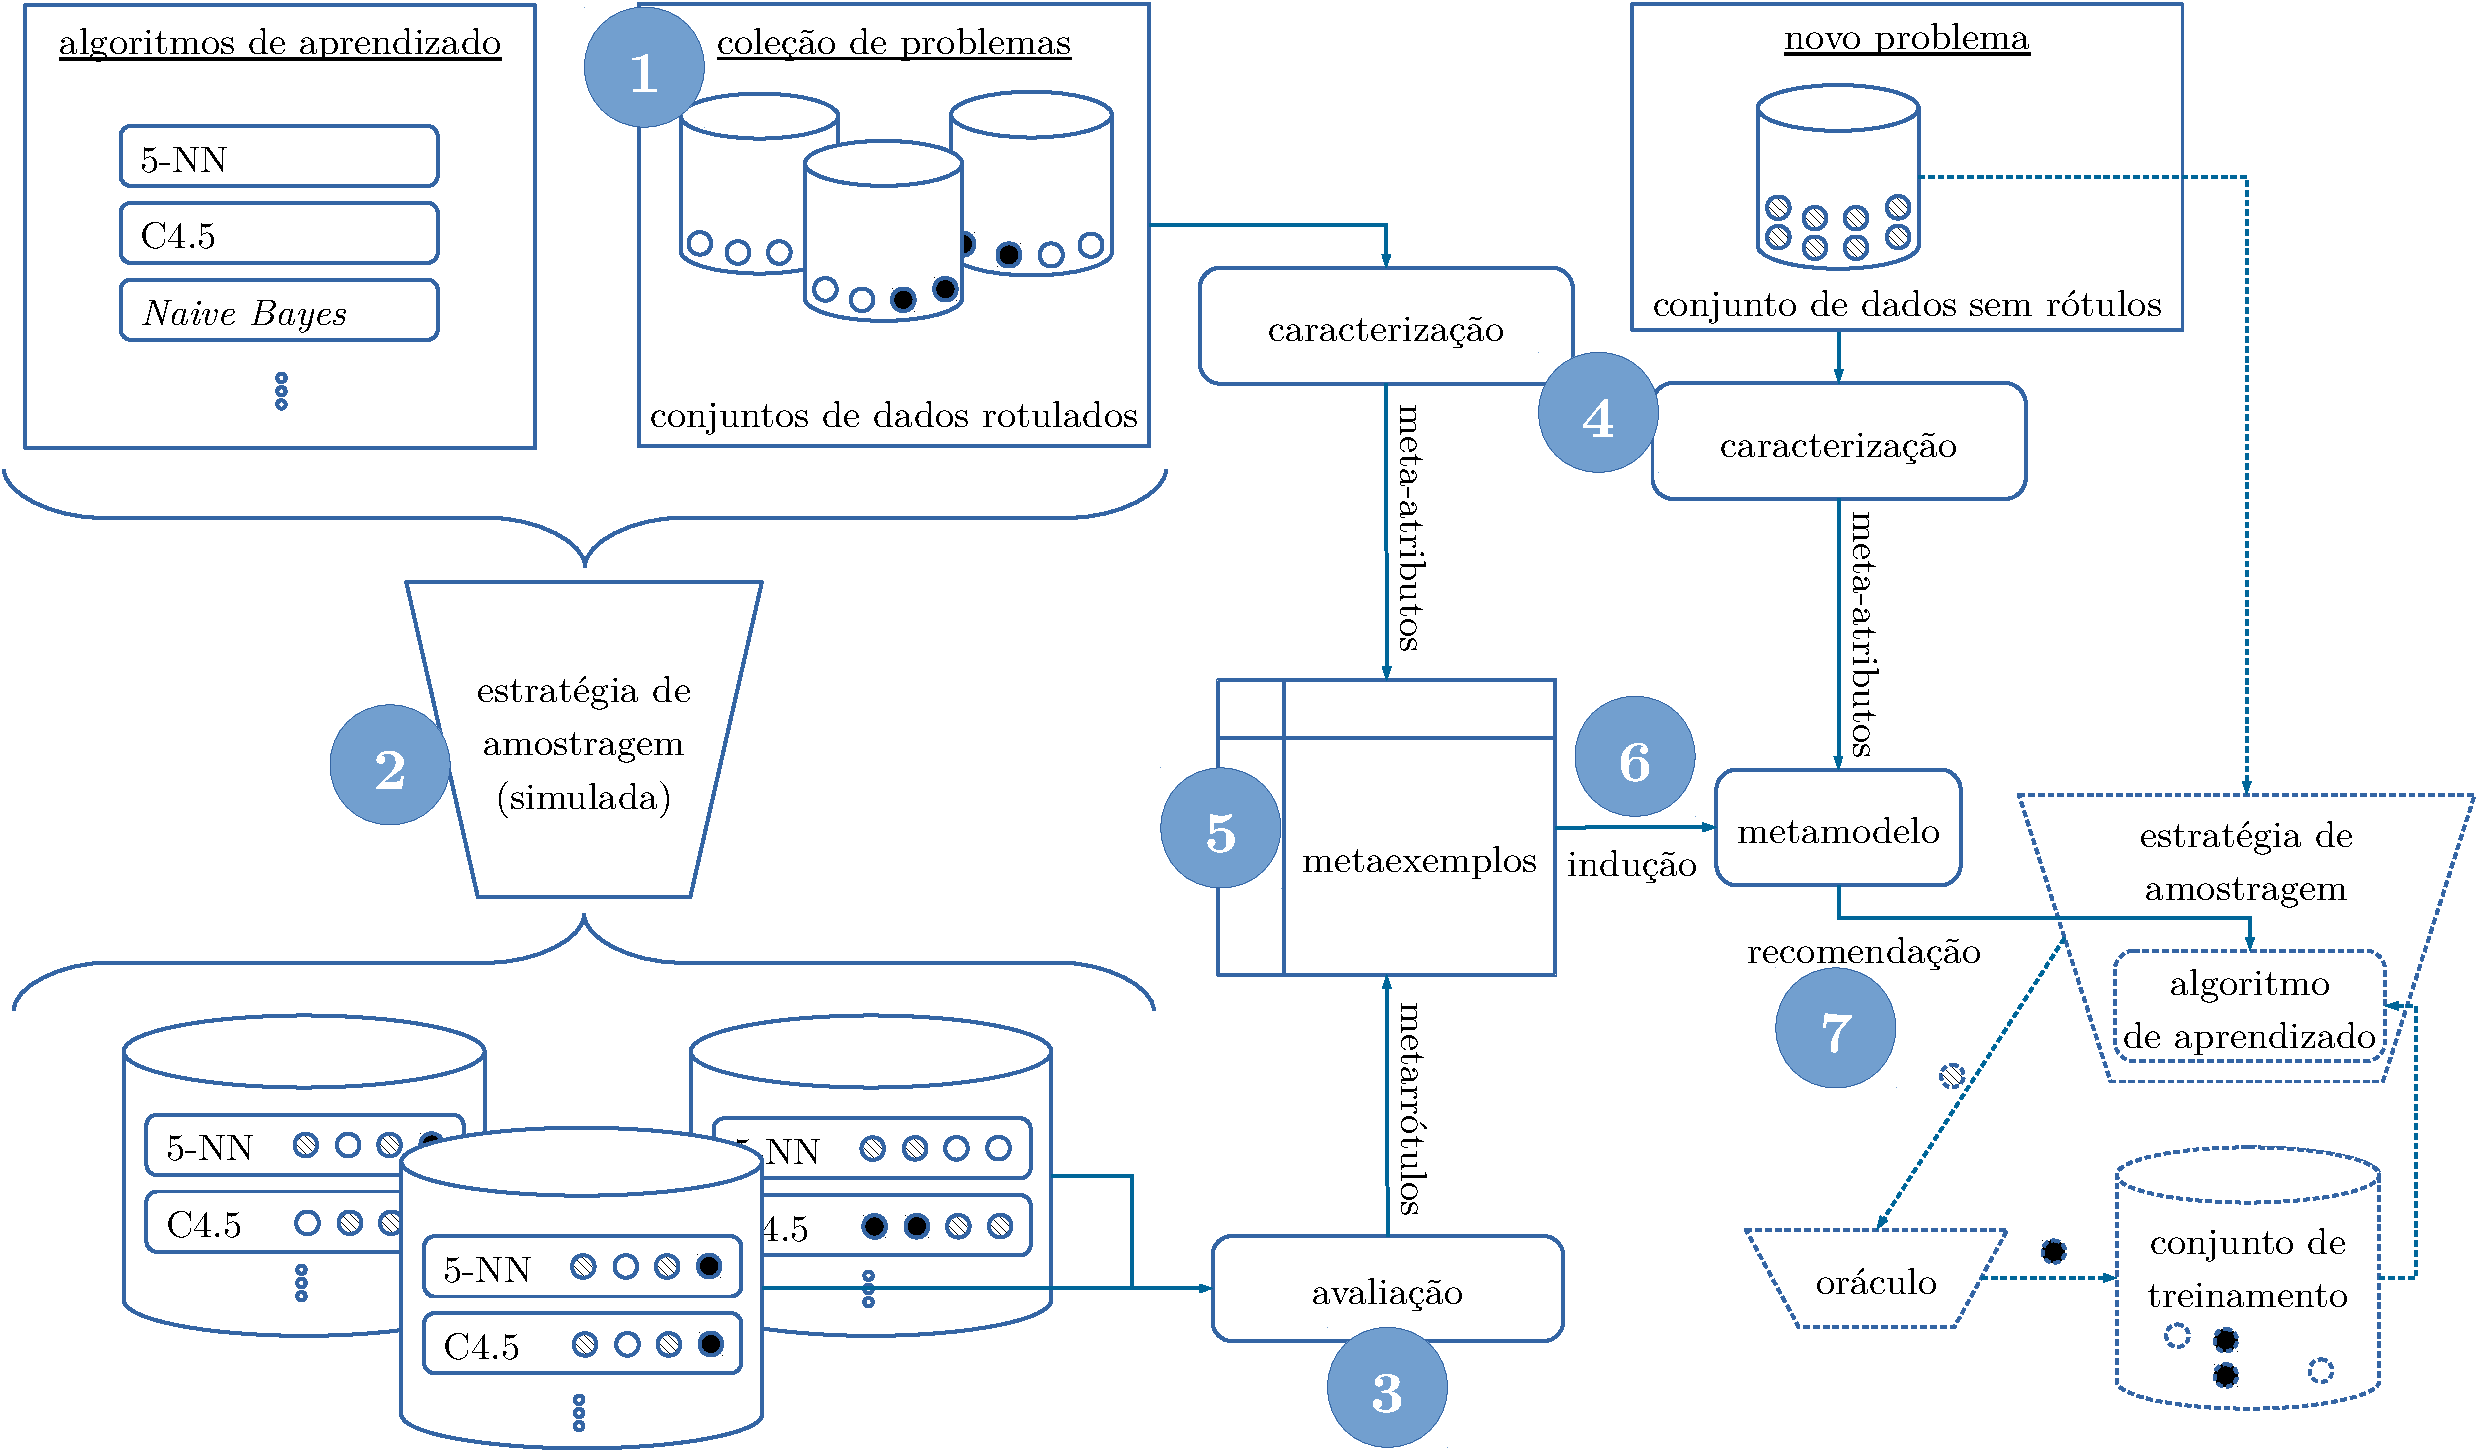
\includegraphics[scale=0.57]{images/meta.pdf}
	\caption[Esquema do sistema de recomendação.]{Esquema do sistema de recomendação. \textit{Os elementos tracejados representam o ciclo usual de aprendizado ativo, que aqui usufrui do meta-aprendizado. Nessa proposta inicial, a estratégia é sempre a mesma.}}
	\label{esquema}
\end{figure}
\end{landscape}

A obtenção de informações sobre o desempenho de estratégias em conjuntos já rotulados requer a caracterização destes (Passo \ref{passo4}).
A caracterização ocorre por meio da extração de medidas que descrevam os dados, chamadas \textit{meta-atributos}.
Uma vez caracterizados, os conjuntos tornam-se comparáveis entre si e viáveis para a construção de um metaconjunto de treinamento, pois passaram a ser representados num mesmo espaço de meta-atributos, como metaexemplos (Passo \ref{passo5}).
O metamodelo induzido com os metaexemplos (Passo \ref{passo6}) é, então, capaz de fazer recomendações de algoritmos (Passo \ref{passo7}) para a estratégia de amostragem ativa (não mais simulada).

Usualmente, medidas estatísticas simples, como \textit{assimetria} e \textit{curtose} são calculadas para cada atributo numérico do conjunto de dados.
Essas medidas estão presentes no STATLOG (Seção \ref{direta}), um dos primeiros sistemas de meta-aprendizado.
Ele contempla conjuntos de dados com diferentes quantidades de atributos numéricos, criando um meta-atributo para cada medida.
Assim, cada meta-atributo consiste na média dos valores da medida ao longo de todos os atributos numéricos.
Segundo \citeonline{kalousis2002algorithm}, essa abordagem por médias incorre em perda de poder discriminatório.
Sua alternativa foi a adoção de histogramas com a contagem de ocorrências em determinadas faixas de valores.
Nesta tese, devido à impossibilidade de prever o intervalo total de ocorrência dos valores e definir seu particionamento, optou-se por substituir o esquema de histogramas por um esquema limitado a alguns valores relevantes.
Esses valores seriam o mínimo, o máximo, o médio e a razão entre o mínimo e o máximo.
Na presente proposta, as medidas escolhidas para caracterização dos conjuntos foram obtidas de alguns trabalhos da literatura de meta-aprendizado.
As medidas são descritas no Quadro \ref{metats}.
\begin{quadro}
\simbolo{\qatt,\qexe,\qnc,\qexeatt,\pno,\lgqexe,\lgqexeatt,\qnom_{min},\qnom_{max},\qnom_{mea},\qnom_{min/max},{\mu}_{min},{\mu}_{max},{\mu}_{mea},{\mu}_{min/max}}{meta-atributos descritos no Quadro \ref{metats} (parte 1/4)}
\simbolo{\sigma_{min},\sigma_{max},\sigma_{mea},\sigma_{min/max},\en_{min},\en_{max},\en_{mea},\en_{min/max},\rho_{min},\rho_{max},\rho_{mea},\rho_{min/max}}{meta-atributos descritos no Quadro \ref{metats} (parte 2/4)}
\simbolo{\sk_{min},\sk_{max},\sk_{mea},\sk_{min/max},\ku_{min},\ku_{max},\ku_{mea},\ku_{min/max},\cn_{k1},\cn_{k1.5},\cn_{k2},\cn_{h1},\cn_{h1.5},\cn_{h2}}{meta-atributos descritos no Quadro \ref{metats} (parte 3/4)}
\simbolo{\du_{k1},\du_{k1.5},\du_{k2},\du_{h1},\du_{h1.5},\du_{h2},\si_{k1},\si_{k1.5},\si_{k2},\si_{h1},\si_{h1.5},\si_{h2}}{meta-atributos descritos no Quadro \ref{metats} (parte 4/4)}
\centering
% \renewcommand\tablename{Quadro}
\caption{Descrição dos 53 meta-atributos.}
\label{metats}
\begin{threeparttable}
\begin{tabular}{|p{3.6cm}|p{4.6cm}|m{6cm}|}
\hline
\textbf{Meta-atributo} & \textbf{Descrição}&\textbf{Fórmula} \\ \hline
$\qatt$ & número de atributos\tnote{a} & $|\mathcal{A}|$ \\ \hline
$\qexe$ & número de exemplos\tnote{a} & $|\mathcal{U}|$ \\ \hline

$\qnc$ & número de classes\tnote{b} & $|Y|$ \\ \hline

$\qexeatt$ & proporção de exemplos para atributos\tnote{c} &
$\frac{|\mathcal{U}|}{|\mathcal{A}|}$
\\ \hline

$\pno$ & proporção de atributos nominais\tnote{c} & 
$\frac{1}{|\mathcal{A}|}|\{A\in \mathcal{A} \mid \nom(A)=1\}|$ \\ \hline

$\lgqexe$ & logaritmo do número de exemplos\tnote{d} &
$\log|\mathcal{U}|$ \\ \hline

$\lgqexeatt$ & logaritmo da proporção exemplos/atributos\tnote{d} &
$\log\frac{|\mathcal{U}|}{|\mathcal{A}|}$ \\ \hline


$\qnom_{min}$, $\qnom_{max}$, $\qnom_{mea}$, $\qnom_{min/max}$ & 
qtd. de valores nominais:\tnote{c}\phantom{c} 
\textit{mínima, máxima, média e mín./máx. por atributo\tnote{c'}\phantom{c'}} &
$\qnom_{A} = |A|, A \in \mathcal{A}$ \\ \hline


${\mu}_{min}$, ${\mu}_{max}$, ${\mu}_{mea}$, ${\mu}_{min/max}$ &
média\tnote{c}\phantom{c} (\textit{idem}) & 
$\mu_j = \frac{1}{|\mathcal{U}|} \sum\limits_{\bm{x} \in \mathcal{U}} x_j$
$1 \leq j \leq |\mathcal{A}|$ \\ \hline

$\sigma_{min}$, $\sigma_{max}$, $\sigma_{mea}$, $\sigma_{min/max}$ &
desvio padrão\tnote{b}\phantom{b} (\textit{idem}) & 
$\sigma_j = \frac{1}{|\mathcal{U}|} \sum\limits_{\bm{x} \in \mathcal{U}}(x_j - \mu_j)^2$
\\ \hline

$\en_{min}$, $\en_{max}$, $\en_{mea}$, $\en_{min/max}$ &
entropia normalizada\tnote{b}\phantom{b} (\textit{idem}) & 
$\en_j = \frac{-1}{\log|\mathcal{U}|} \sum\limits_{\bm{x} \in \mathcal{U}} x_j\log x_j$
\\ \hline

% pearson
$\rho_{min}$, $\rho_{max}$, $\rho_{mea}$, $\rho_{min/max}$ &
correlação entre pares de atributos\tnote{b}\phantom{b} (\textit{idem}) & 
$\rho_{jk} = $ \phantom{ooooooooooo} \phantom{oooooooo}
$(\sigma_j^2\cdot\sigma_k^2)^{-\frac{1}{2}}
\sum\limits_{\bm{x} \in \mathcal{U}} 
(x_j - \mu_j)(x_k - \mu_k)$ \\ \hline

$\sk_{min}$, $\sk_{max}$, $\sk_{mea}$, $\sk_{min/max}$ &
assimetria\tnote{b}\phantom{b} (\textit{idem}) & 
$ \sk_j = \frac{n}{(n -1)(n - 2)} \sum\limits_{\bm{x} \in \mathcal{U}}
\frac{(x_j - \mu_J)^3}{\sigma_j^3}$
\\ \hline

$\ku_{min}$, $\ku_{max}$, $\ku_{mea}$, $\ku_{min/max}$ &
curtose\tnote{b}\phantom{b} (\textit{idem}) & 
\makecell{$\ku_j =  \frac{n(n+1)}{(n -1)(n - 2)(n-3)}
\sum\limits_{\bm{x} \in \mathcal{U}}
\frac{(x_i - \mu_j)^4}{\sigma_j^4}$\\
$- 3(n-1)^2[(n-2)(n-3)]^{-1}$} \\ \hline

% Internal evaluation
% dunn: compactação e separação; silhueta: ?
$\cn_{k1}$, \phantom{ll}$\cn_{k1.5}$, \phantom{ll}$\cn_{k2}$,
$\cn_{h1}$, \phantom{ll}$\cn_{h1.5}$, \phantom{ll}$\cn_{h2}$ &
conectiv.\tnote{e}\phantom{e} \textit{k-médias} \phantom{oooo}
conectiv \textit{agrup. hierárq.} & 
agrupam. \cite{xu2008clustering}
\textit{qtd. de grupos: $|Y|$; $1,5|Y|$ e $2|Y|$}\\
\hline

$\du_{k1}$, \phantom{l}$\du_{k1.5}$, \phantom{l}$\du_{k2}$,
$\du_{h1}$, \phantom{l}$\du_{h1.5}$, \phantom{l}$\du_{h2}$ &
índ. Dunn\tnote{e}\phantom{e} \textit{k-médias} \phantom{ooo}
índ. Dunn \textit{agr. hierárq.} &
agrupam. \cite{dunn1973fuzzy} \phantom{oooooo} (\textit{idem}) \\ \hline


$\si_{k1}$, \phantom{aa}$\si_{k1.5}$, \phantom{aa}$\si_{k2}$,
$\si_{h1}$, \phantom{aa}$\si_{h1.5}$, \phantom{aa}$\si_{h2}$ &
silhueta\tnote{e}\phantom{e} \textit{k-médias} \phantom{ooooo}
silhueta \textit{agrup. hierárq.} &
agrupam. \cite{rousseeuw1987silhouettes} (\textit{idem}) \\ \hline

\end{tabular}
\begin{tablenotes}
\item [a] Caracterização sugerida por \citeonline{conf/ijcai/RendellST87}.
\item [b] Baseado no projeto STATLOG \cite{brazdil1994analysis}.
\item [c] Baseado no conjunto de \citeonline{kalousis2002algorithm}.
\item [c'] Adaptação da sumarização proposta por \citeonline{kalousis2002algorithm}.
\item [d] Meta-atributos para recomendar algoritmos de agrupamento \cite{conf/ijcnn/SoutoPSACLS08}.
\item [e] Meta-atributos para recomendação de algoritmos de classificação \cite{souza2010meta}
e de algoritmos de agrupamento \cite{Ferrari2015181}.
\end{tablenotes}
\end{threeparttable}

\end{quadro}

\simbolo{\gamma}{metaclasse}
\simbolo{\chi}{metaexemplo}
\simbolo{\Lambda}{metaconjunto de dados}
\simbolo{\eta}{metamodelo}
\simbolo{\psi(\Lambda)}{função indutora para o metaconjunto de dados $\Lambda$}
Finalmente, o esquema proposto segue o Algoritmo \ref{algmta}.
O esquema é o mesmo nas demais formas de recomendação, com pequenas alterações triviais.
Na recomendação de estratégias, escolhe-se um algoritmo de antemão e, na recomendação de pares estratégia-algoritmo, ambos compõem a informação de metaclasse.
\begin{algoritmo}
\caption{Recomendação automática de algoritmos de aprendizado.}
  \small
\label{algmta}
\Entrada{
 \\ $\Phi$ - conjunto de funções indutoras $\phi$ (algoritmos)
 \\ $\mathfrak{L}$ - coleção de conjuntos de dados rotulados
 \\ $\psi$ - função de indução (algoritmo do meta-aprendiz)
 \\ $\cent$ - orçamento (50 ou 100 exemplos a rotular)
 \\ $q$ - função-critério que representa a estratégia (Algoritmo \ref{algo})
 \\ $k$ - número de partições da validação cruzada
 \\ $\mathcal{U}$ - novo conjunto de dados sem rótulos
}
\Resultado{
 \\ $\phi$ - função indutora recomendada (algoritmo do aprendiz ativo)
}
\algalg{\treina{$\Phi$, $\mathfrak{L}$, $\psi$, $\cent$, $q$, $k$, $\mathcal{U}$}}{
  $\Lambda\leftarrow\varnothing$\\
  \ForEach {$\mathcal{L}\in\mathfrak{L}$}{    
    $\gamma=$ \best{$\Phi$, $\mathcal{L}$, $\cent$, $q$, $k$} \come{metaclasse}\\    
    $\bm{\chi} = (\qatt,\qexe,\qnc,\qexeatt,\pno,\lgqexe,\lgqexeatt,\qnom_{min},\qnom_{max},\qnom_{mea},\qnom_{min/max},$ 
    \phantom{$\bm{\chi}= ($}${\mu}_{min},{\mu}_{max},{\mu}_{mea},{\mu}_{min/max},\sigma_{min},\sigma_{max},\sigma_{mea},\sigma_{min/max},$
    \phantom{$\bm{\chi}= ($}$\en_{min},\en_{max},\en_{mea},\en_{min/max},\rho_{min},\rho_{max},\rho_{mea},\rho_{min/max},$
    \phantom{$\bm{\chi}= ($}$\sk_{min},\sk_{max},\sk_{mea},\sk_{min/max},\ku_{min},\ku_{max},\ku_{mea},\ku_{min/max},$
    \phantom{$\bm{\chi}= ($}$\cn_{k1},\cn_{k1.5},\cn_{k2},\cn_{h1},\cn_{h1.5},\cn_{h2},\du_{k1},\du_{k1.5},\du_{k2},\du_{h1},\du_{h1.5},\du_{h2},$
    \phantom{$\bm{\chi}= ($}$\si_{k1},\si_{k1.5},\si_{k2},\si_{h1},\si_{h1.5},\si_{h2})$ \come{meta-atributos extraídos de $\mathcal{L}$}\\
%     Usei parêntesis porque pode ser um vetor, já que todos os meta-atributos são numéricos.
    $\Lambda\leftarrow\Lambda\cup\{\langle \bm{\chi},\gamma\rangle\}$
  }
  $\eta\leftarrow\psi(\Lambda)$ \come{induz metamodelo} \\
  \Return $\eta$
}
\algalg{\recomenda{$\eta$, $\cent$, $\mathcal{U}$}}{
	$\bm{\chi}= (\qatt, ...,\si_{h2})$ \come{meta-atributos extraídos de $\mathcal{U}$}\\
	$\phi \leftarrow \hat{y}_{\eta}(\bm{\chi})$\\
  \Return $\phi$
}
\end{algoritmo}


% % 
% % ;
% % \ano{\cite{conf/ijcnn/SoutoPSACLS08}, sobre clustering,
% % ``melhoram`` statlog, aplicando log}
% 

\section{Considerações}
Neste capítulo, as estratégias ATU e HTU foram propostas juntamente com a adaptação SGmulti e o sistema de recomendação baseado em meta-aprendizado.
Todas as propostas foram textualmente e algoritmicamente descritas.
No Quadro \ref{strats}, as novas estratégias são incorporadas à lista comparativa de estratégias previamente descritas no Capítulo \ref{contexto}.
\begin{quadro}
\caption[Características de cada estratégia, incluindo propostas.]{Características de cada estratégia, incluindo estratégias propostas (em negrito).}
\label{strats}
\centering
\begin{threeparttable}
\begin{tabular}{|l|p{3cm}|p{2cm}|l|p{3.2cm}|}
\hline
\textbf{Estratégia}		& \textbf{Busca}		&\textbf{Aprendiz}  & \textbf{Dependência}		&\textbf{Complexidade}  \\ \hline
Rnd\tnote{a}			& {exploratória aleatória} 		& ausente			& nenhuma							&dispensa treinamento  \\ \hline
\textbf{ATU}\tnote{k}			&{exploratória}		& sem aprendiz				& nenhuma 							&dispensa treinamento  \\ \hline
HS\tnote{b}			&{balanceada exploratória prospectiva}	& ausente		& total							&dispensa treinamento\tnote{*}  \\ \hline
Mar/Ent\tnote{a} /QBC\tnote{c}	& prospectiva					& presente		& total							&$\mathcal{O}(1)$  \\ \hline
DW\tnote{d}			& prospectiva					& presente		& total							&$\mathcal{O}(1)$  \\ \hline
EER\tnote{e}			& prospectiva					& presente	& total							&$\mathcal{O}(|Y||\mathcal{U}|^2)$  \\ \hline
TU\tnote{f}			&{balanceada exploratória prospectiva}	& presente		& total							&$\mathcal{O}(1)$  \\ \hline
SGnetwork\tnote{g}		&{limitada exploratória aleatória}	& presente			& total							&$\mathcal{O}(1)$  \\ \hline
\textbf{SGmulti}\tnote{g}		&{limitada exploratória aleatória}	& presente			& total							&$\mathcal{O}(|Y|)$  \\ \hline
SVMsim\tnote{h}			& prospectiva					&{presente \phantom{oooo} específico}	& total							&$\mathcal{O}(|\mathcal{L}||\mathcal{U}|)$  \\ \hline
EGL\tnote{i}			& prospectiva					&{presente \phantom{oooo} específico}	& total							&$\mathcal{O}(|Y||\mathcal{U}|)$  \\ \hline
SVMbal\tnote{j}			&{combinada exploratória prospectiva}&{presente \phantom{oooo} específico}			& total							&$\mathcal{O}(|\mathcal{L}||\mathcal{U}|)$  \\ \hline
\textbf{HTU}\tnote{k}			&{combinada exploratória prospectiva}&{combinação \phantom{oo} ausente\phantom{oooo} presente}	&{total}			&$\mathcal{O}(1)$  \\ 
\hline
\end{tabular}
\begin{tablenotes}
\item [*] Na ausência de aprendiz não há treinamento, porém HS tem sua própria complexidade a ser considerada.
\item [a] Amostragem aleatória, por margem ou entropia \cite{series/synthesis/2012Settles}.
\item [b] Amostragem hierárquica \cite{journals/tcs/Dasgupta11}.
\item [c] Consulta por comitê \cite{conf/icml/AbeM98}.
\item [d] Amostragem ponderada por densidade \cite{settles2008curious}.
\item [e] Redução esperada do erro \cite{conf/ijcai/GuoG07}.
\item [f] Amostragem ponderada por densidade e utilidade de treinamento \cite{settles2010active,journals/coling/FujiiITT98}.
% \item [g] SGnetwork \cite{journals/ml/CohnAL94}.
\item [g] SGmulti \cite{conf/hais/SantosC14}.
\item [h] Margem simples \cite{journals/jmlr/TongK01}.
\item [i] Comprimento esperado do gradiente \cite{conf/nips/SettlesCR07}.
\item [j] Balanceamento exploração-prospecção \cite{conf/icdm/OsugiKS05}.
\item [k] Amostragem ponderada por densidade sem aprendiz e híbrida \cite{bracis15}.
\end{tablenotes}
\end{threeparttable}
\end{quadro}

Resumidamente, a estratégia ATU consiste na remoção total do aprendiz de TU.
HTU consiste na ativação do aprendiz somente nos momentos em que o modelo preditivo esteja suficientemente estável, a ponto de manter a correlação entre a medida de incerteza e a função-critério de TU acima de um elevado limiar. 
SGmulti apenas estende o conceito da abordagem original, mantendo uma reserva de exemplos artificiais para cada classe.

A tentativa de aprendizado meta-ativo é uma nova abordagem na área de aprendizado ativo - até onde alcança o conhecimento do autor.
Ela é baseada na recomendação automática de algoritmos de aprendizado.
Inicialmente, meta-atributos são extraídos do conjunto de dados, caracterizando-o.
Uma base de conhecimento previamente construída por meio da caracterização de outros conjuntos, cujos melhores algoritmos de aprendizado são conhecidos, é utilizada como metaconjunto.
Idealmente, um metamodelo induzido com esse metaconjunto permitiria predizer qual o melhor  algoritmo e, possivelmente, a melhor estratégia ou o melhor par estratégia-algoritmo.

As propostas aqui apresentadas foram avaliadas empiricamente de acordo com o método descrito no Capítulo \ref{metodologia}.


\chapter{Método experimental} \label{metodologia} \thispagestyle{empty}
\epigraph{
\textit{Bien loin que l'objet précède le point de vue, on dirait que c'est le point de vue qui crée l'objet}\ldots
}{Ferdinand de Saussure\footnotemark[1]}
\setcounter{footnote}{1}
\footnotetext[1]{\aspas{Bem longe de dizer que o objeto precede o ponto de vista, diríamos que é o ponto de vista que cria o objeto\ldots}
- \citeonline{saussure1972curso}, sobre as peculiaridades metodológicas em sua área de estudo.}
% Bien loin que l'objet précède le point de vue, on dirait que c'est le point de vue qui crée l'objet, et d'ailleurs rien ne nous dit d'avance que l'une de ces manières de considérer le fait en question soit antérieure ou supérieure aux autres.\cite{godel1957sources}
% Bem longe de dizer que o objeto precede o ponto de vista, diríamos que é o ponto de vista que cria o objeto; aliás, nada nos diz de antemão que uma dessas maneiras de considerar o fato em questão seja anterior ou superior às outras.
% \ano{corrected t test p/ avaliar 2 algs em 1 dataset; wilcoxon em vários}
As escolhas metodológicas expostas neste capítulo fundamentam a avaliação experimental das propostas deste trabalho.
% para identificar os pontos críticos na escolha de estratégias e também para comprovação empírica.
Na Seção \ref{desccen}, são apresentados detalhes sobre o cenário adotado.
Os conjuntos de dados, utilizados visando a simulação de aplicações reais, são descritos e analisados sob diferentes aspectos na Seção \ref{desccon}.
Nas seções \ref{learners} e \ref{confstrats}, os parâmetros são definidos e considerações são feitas sobre as estratégias de amostragem ativa e os algoritmos de aprendizado empregados - respectivamente.
As medidas de desempenho, a forma de validação e o tipo de teste empregado para a avaliação da significância estatística dos resultados experimentais são apresentados na Seção \ref{avaliacao}.
Na Seção \ref{sec:curvas}, são introduzidas as curvas de ranqueamento - importante contribuição metodológica deste trabalho.
Por fim, a Seção \ref{sec:consider} contém as considerações gerais.
\usetikzlibrary{trees}

Parte das decisões tomadas foram baseadas num experimento preliminar.
Ele permitiu a definição de experimentos definitivos adequados aos recursos computacionais disponíveis.
% Nesse teste inicial, dez estratégias de aprendizado ativo
% % (C4.5, NB, VFDT e 5-NN)
% foram comparadas.
% Dez execuções de validação cruzada em dez partições totalizaram 100 \pools para cada conjunto - conforme sugerido por \citeonline{conf/pakdd/BouckaertF04}.
% As \pools foram consultadas até o ponto em que a acurácia máxima da melhor estratégia fosse atingida.
Aproximadamente um mês foi necessário para a conclusão do experimento nos 28 menores conjuntos de dados.
Assim, considerando-se o crescimento exponencial do custo computacional em alguns pares estratégia-algoritmo com o aumento do número de classes, atributos e/ou exemplos, foi necessário reduzir a quantidade de iterações do procedimento de validação e antecipar o término das consultas.
Os resultados desse experimento preliminar com relação a desempenho não são reportados nesta tese por serem menos abrangentes que o experimento definitivo.
Mais detalhes podem ser encontrados em \citeonline{conf/hais/SantosC14}.

\section{Cenário escolhido}\label{desccen}
É necessário situar o escopo do presente trabalho, dado o grande número de possibilidades dentro dos cenários e restrições que possam existir num dado problema.
Existem três principais cenários na literatura de aprendizado ativo
\cite{settles2010active}:
\textit{síntese de consulta por associação} ou
\ing{consulta de exemplos sintetizados}{membership query synthesis};
\textit{amostragem baseada em \pool}; e,
\textit{amostragem seletiva baseada em fluxo}.
% Mais detalhes são apresentados no Apêndice \ref{cenarios}.
O cenário adotado neste trabalho é baseado em \pool.
Especificamente, há as seguintes restrições de escopo:
\begin{itemize}
 \item problemas monorrótulo multiclasse;
 \item consulta pela classe (não por valores de atributos, por exemplo);
 \item conjunto ou quantidade de classes possíveis previamente conhecida;
 \item distribuição das classes não necessariamente balanceada;
 \item distribuição estacionária;
 \item custo por erro de classificação uniforme;
 \item custo por consulta uniforme;
 \item oráculo único e sujeito a ruído consistente (sempre comete os mesmos erros);
 \item os domínios dos atributos nominais são previamente conhecidos;
 \item atributos sem valores faltantes; e,
 \item consulta \textit{on-line}, ou seja, um a um.
\end{itemize}
As seguintes condições foram criadas visando maior rigor experimental, replicabilidade e verossimilhança com aplicações reais:
\begin{itemize}
 \item um rótulo inicial por classe;
 \item todo o conjunto de dados original é utilizado no processo de validação cruzada - exceto exemplos duplicados e no caso de EER (Seção \ref{eerconfig}); e,
 \item critério de parada determinado pelo orçamento de cem consultas ($\cent=100$).
 \end{itemize}
Uma condição mínima necessária a diversas estratégias é existir, no modelo de classificação, a capacidade de estimar pelo menos um esboço da fronteira de decisão - vide critérios de consulta no Capítulo \ref{contexto}.
Consequentemente, optou-se pela adoção de um exemplo rotulado inicial por classe.
Além dessa ser a quantidade mínima para que um modelo seja induzido e possa estimar uma fronteira de decisão, ela também reflete a cautela necessária em aplicações reais, pois o aprendizado ativo não garante que exemplos de todas as classes sejam consultados.
Por exemplo, quanto maior o grau de desbalanceamento entre as classes, maior o custo com consultas adicionais necessárias até que todas as classes sejam contempladas.
Portanto, é importante obter criteriosamente alguns rótulos antes de ser iniciado o processo de amostragem ativa.

Uma maneira de obter um rótulo por classe é por meio do \textit{aprendizado guiado} \cite{conf/kdd/AttenbergP10}.
Esse tipo de aprendizado realiza uma amostragem em que o usuário escolhe os exemplos a rotular.
Normalmente, ele sabe de antemão as classes menos frequentes e é capaz de encontrar exemplos correspondentes, seja por meio de consulta a motores de busca na \textit{internet}, da própria memória pessoal ou de outras formas.
Essa modalidade de amostragem faz maior usufruto da capacidade da inteligência humana enquanto agente supervisor do que a simples rotulação.
Embora custoso, esse potencial humano pode ser aproveitado no estágio inicial da rotulação e favorecer a posterior amostragem ativa, minimizando as futuras intervenções humanas.

A prática de rotulação prévia em experimentos também tem sido parte do método experimental adotado em outros trabalhos \cite{conf/nips/GuoS07, conf/cvpr/BiswasP13, conf/iconip/GuJC14a}, com variações mais permissivas com relação à quantidade de exemplos \cite{journals/prl/PatraB12} ou substituída por uma amostragem aleatória aplicada até que se encontre um exemplo de cada classe \cite{chermanaprendizado}.

A limitação a um número fixo de consultas segue a observação de \citeonline{series/synthesis/2012Settles} sobre o critério desejável de parada do processo de aprendizado ativo. 
Ele relata que, em aplicações reais, normalmente trata-se de uma restrição financeira.
Consequentemente, a definição do orçamento para fins experimentais tem sido arbitrária na literatura, sendo 100 consultas um valor recorrente \cite{journals/pieee/CrawfordTY13,chermanaprendizado,conf/nips/SettlesCR07,conf/icml/RoyM01,conf/emnlp/SettlesC08}.
 
Outra característica presente nos experimentos está no não aproveitamento da informação de orçamento disponível - decisão usual na literatura \cite{conf/icml/RoyM01}.
Isso implica na geração de sequências de consultas provavelmente não ótimas, ou, em outras palavras, cada consulta é realizada como se fosse a última.
Uma consulta ótima dependeria de quantas ainda poderiam ser feitas.
Apesar de ser uma possibilidade teórica, seu não aproveitamento não é uma limitação real, pois não é esperado que existam estratégias capazes de tirar proveito dessa informação de forma significativa.

\section{Conjuntos de dados}\label{desccon}
Os conjuntos de dados do projeto de \citeonline{doi/ucipp}, baseado no repositório da \sigla{UCI}{Universidade da Califórnia, Irvine} - \cite{bache2013uci}, foram utilizados com o objetivo de representar os variados domínios existentes em aplicações reais.
Parte dos conjuntos foi descartada conforme descrito nas seções \ref{sectempo} e \ref{secsimi}.
Os critérios de descarte objetivaram selecionar os conjuntos mais adequados\footnote{Análises posteriores à primeira versão deste documento demonstraram uma importante deficiência na coleção adotada (Apêndice \ref{apflu}).} para a coleção utilizada nos experimentos desta tese.
Contudo, a análise dos experimentos leva em conta que o propósito da construção de uma coleção representativa de conjuntos de dados não é a demonstração da superioridade de algum algoritmo em todos os casos, mas identificar os pontos fortes de cada algoritmo  \cite{books/cu/Japkowicz2011}.
% The purpose of data set selection should not be to demonstrate an algorithm’s superiority to another in all cases, but rather to identify the areas of strengths of various algorithms with respect to domain characteristics or on specific domains of interest.

\subsection{Custo computacional}\label{sectempo}
Dada a quantidade envolvida de estratégias de amostragem ativa, algoritmos de aprendizado e execuções de validação por conjunto de dados (Seção \ref{validacao}), a limitação do tempo de processamento foi essencial para que os experimentos previstos fossem realizados.
Essa limitação não afetou os experimentos, pois o foco é a acurácia preditiva.
Logo, os conjuntos de dados que demandam excessivo tempo para a inicialização de estratégias ou para a realização de consultas foram descartados, permitindo a viabilidade computacional dos experimentos.
Esse tempo foi estimado por meio de um experimento reduzido.
Ele consistiu na execução de validação cruzada em duas partes aplicada apenas ao algoritmo com maior custo computacional (RoF - Seção \ref{learners}) e três estratégias, cada uma com sua respectiva particularidade referente ao custo computacional:
\begin{itemize}
   \item ATU - inicialização requer quantidade quadrática de cálculos de distância em relação ao tamanho da reserva de exemplos;
   \item SGmulti - consulta requer quantidade de treinamentos proporcional ao número de classes; e,
   \item EER - consulta requer quantidade de treinamentos proporcional ao número de classes e quadrática com relação ao número de exemplos.
\end{itemize}
Os seguintes conjuntos de dados foram descartados, uma vez que atingiram um tempo de processamento entre 4 e 16 horas para as primeiras 50 consultas no experimento reduzido:
% +ou- ordenado por tempo
\textit{arcene, micro mass pure spectra, micro mass mixed spectra, multiple features, digits2, lsvt voice rehabilitation, semeion, cnae 9, gas drift, gas drift different concentrations} e \textit{hill valley with noise}.
Estimou-se um tempo entre 700 e 2800 dias para cada um desses conjuntos no experimento definitivo, tomando por base as seguintes considerações:
\begin{itemize}
   \item 100 consultas contêm 3 vezes mais unidades de treinamento\footnote{Quantidade de exemplos de treinamento. Todos são reaprendidos a cada nova consulta.} que 50 consultas;
   \item seriam avaliados, no pior caso, 8 algoritmos e 14 estratégias; e,
   \item o processo de validação consistiria de 25 execuções.
\end{itemize}
Mesmo dividindo esses valores estimados de duração do experimento definitivo pelo número de núcleos de processamento inicialmente disponíveis, 100, não seria viável incluir tais conjuntos de dados.

\subsection{Similaridade}\label{secsimi}
Conjuntos de dados equivalentes ou muito similares foram excluídos dos experimentos desta tese com a finalidade de aumentar a \textit{independência entre amostras} para o teste estatístico (seções \ref{testestbase} e \ref{testestmeta}).
A ausência de redundância entre os conjuntos também é importante para a avaliação adequada da capacidade de generalização do meta-aprendizado: tal como no nível base, metaexemplos não devem aparecer simultaneamente nos conjuntos de teste e treinamento.
A similaridade entre conjuntos foi indiretamente estimada do ponto de vista do viés de aprendizado.
Trata-se de uma escolha conservadora, pois os mesmos vieses podem ser adequados a problemas distintos.
Essa abordagem é baseada na tabela de distâncias entre taxas de erro empregada por \citeonline{brazdil1994analysis}.
Neste trabalho, entretanto, optou-se pela comparação de desempenhos relativos, feita por uma medida de correlação, pois ela proporciona a análise de um ponto de vista mais amplo, independente de valores absolutos de acurácia, por exemplo.
% Brazdil faz tabela de distâncias pareadas com taxas de erro sendo
% as dimensões, depois faz decomposição ortogonal para visualizar em duas dimensões.
% Depois ele faz agrupamento hierárquico.

A correlação de Spearman \cite{reference/stat/GibbonsC11} foi calculada entre os ranqueamentos médios de desempenho de 10 algoritmos de aprendizado (Seção \ref{learners}) com o objetivo de estimar indiretamente a similaridade entre cada par de conjuntos.
A medida de desempenho adotada, $\kappa$ (Seção \ref{newhtu}), foi obtida em 100 execuções de validação cruzada em dez partes.
Valores elevados de correlação foram obtidos devido à frequente superioridade de alguns algoritmos sobre outros  \cite{journals/jmlr/DelgadoCBA14}.
Valores acima de $0,95$ foram considerados indicativos de similaridade excessiva.
Esse foi o maior valor atingido por conjuntos de domínios conhecidamente distintos.

Apenas um conjunto dentre cada grupo de conjuntos similares permaneceu e os demais foram descartados.
Os conjuntos descartados são listados a seguir:
\textit{thyroid allrep, thyroid allhyper, thyroid allhypo, thyroid allbp, thyroid dis, robot failure lp4, leukemia haslinger, robot nav sensor readings 4, cardiotocography 10class, nursery 4class, movement libras 10, mushroom expanded, waveform v1, connectionist vowel reduced, breast tissue 6class, yeast, wine quality 5class, abalone 11class, robot nav sensor readings 24} e variações dos conjuntos \textit{volcanoes} \textit{a}, \textit{b}, \textit{d} e \textit{e}.
Conjuntos em que todos os algoritmos obtiveram um desempenho próximo ao acaso ($\kappa < 0,02$) poderiam gerar colocações de ranqueamento de pares estratégia-algoritmo espúrias, afetando os resultados sem trazer qualquer benefício para os experimentos.
Consequentemente, eles também foram descartados: \textit{autoUniv-au6-1000, autoUniv-au6-1000, autoUniv-au6-250-drift-au6-cd1-500, meta-data, planning-relax} e \textit{monks2}.

A Figura \ref{datasetsimistodos} contém o mapa de calor \cite{wilkinson2009history} que atribui uma intensidade de correlação a cada par dentre os 90 conjuntos de dados que restaram ao fim do processo de descarte.
Este e os demais mapas de calor neste texto estão com as linhas ordenadas pela soma dos valores nas colunas.
O azul e o vermelho mais intensos indicam, respectivamente, o melhor e o pior valor.
A cor branca indica o valor central.
No presente caso, o melhor valor é o mais baixo; em valores de acurácia, distância e correlação na predição de ranqueamentos, o melhor valor é o mais elevado. 
\begin{figure}
  \setlength{\unitlength}{1.0cm}
  \centering
    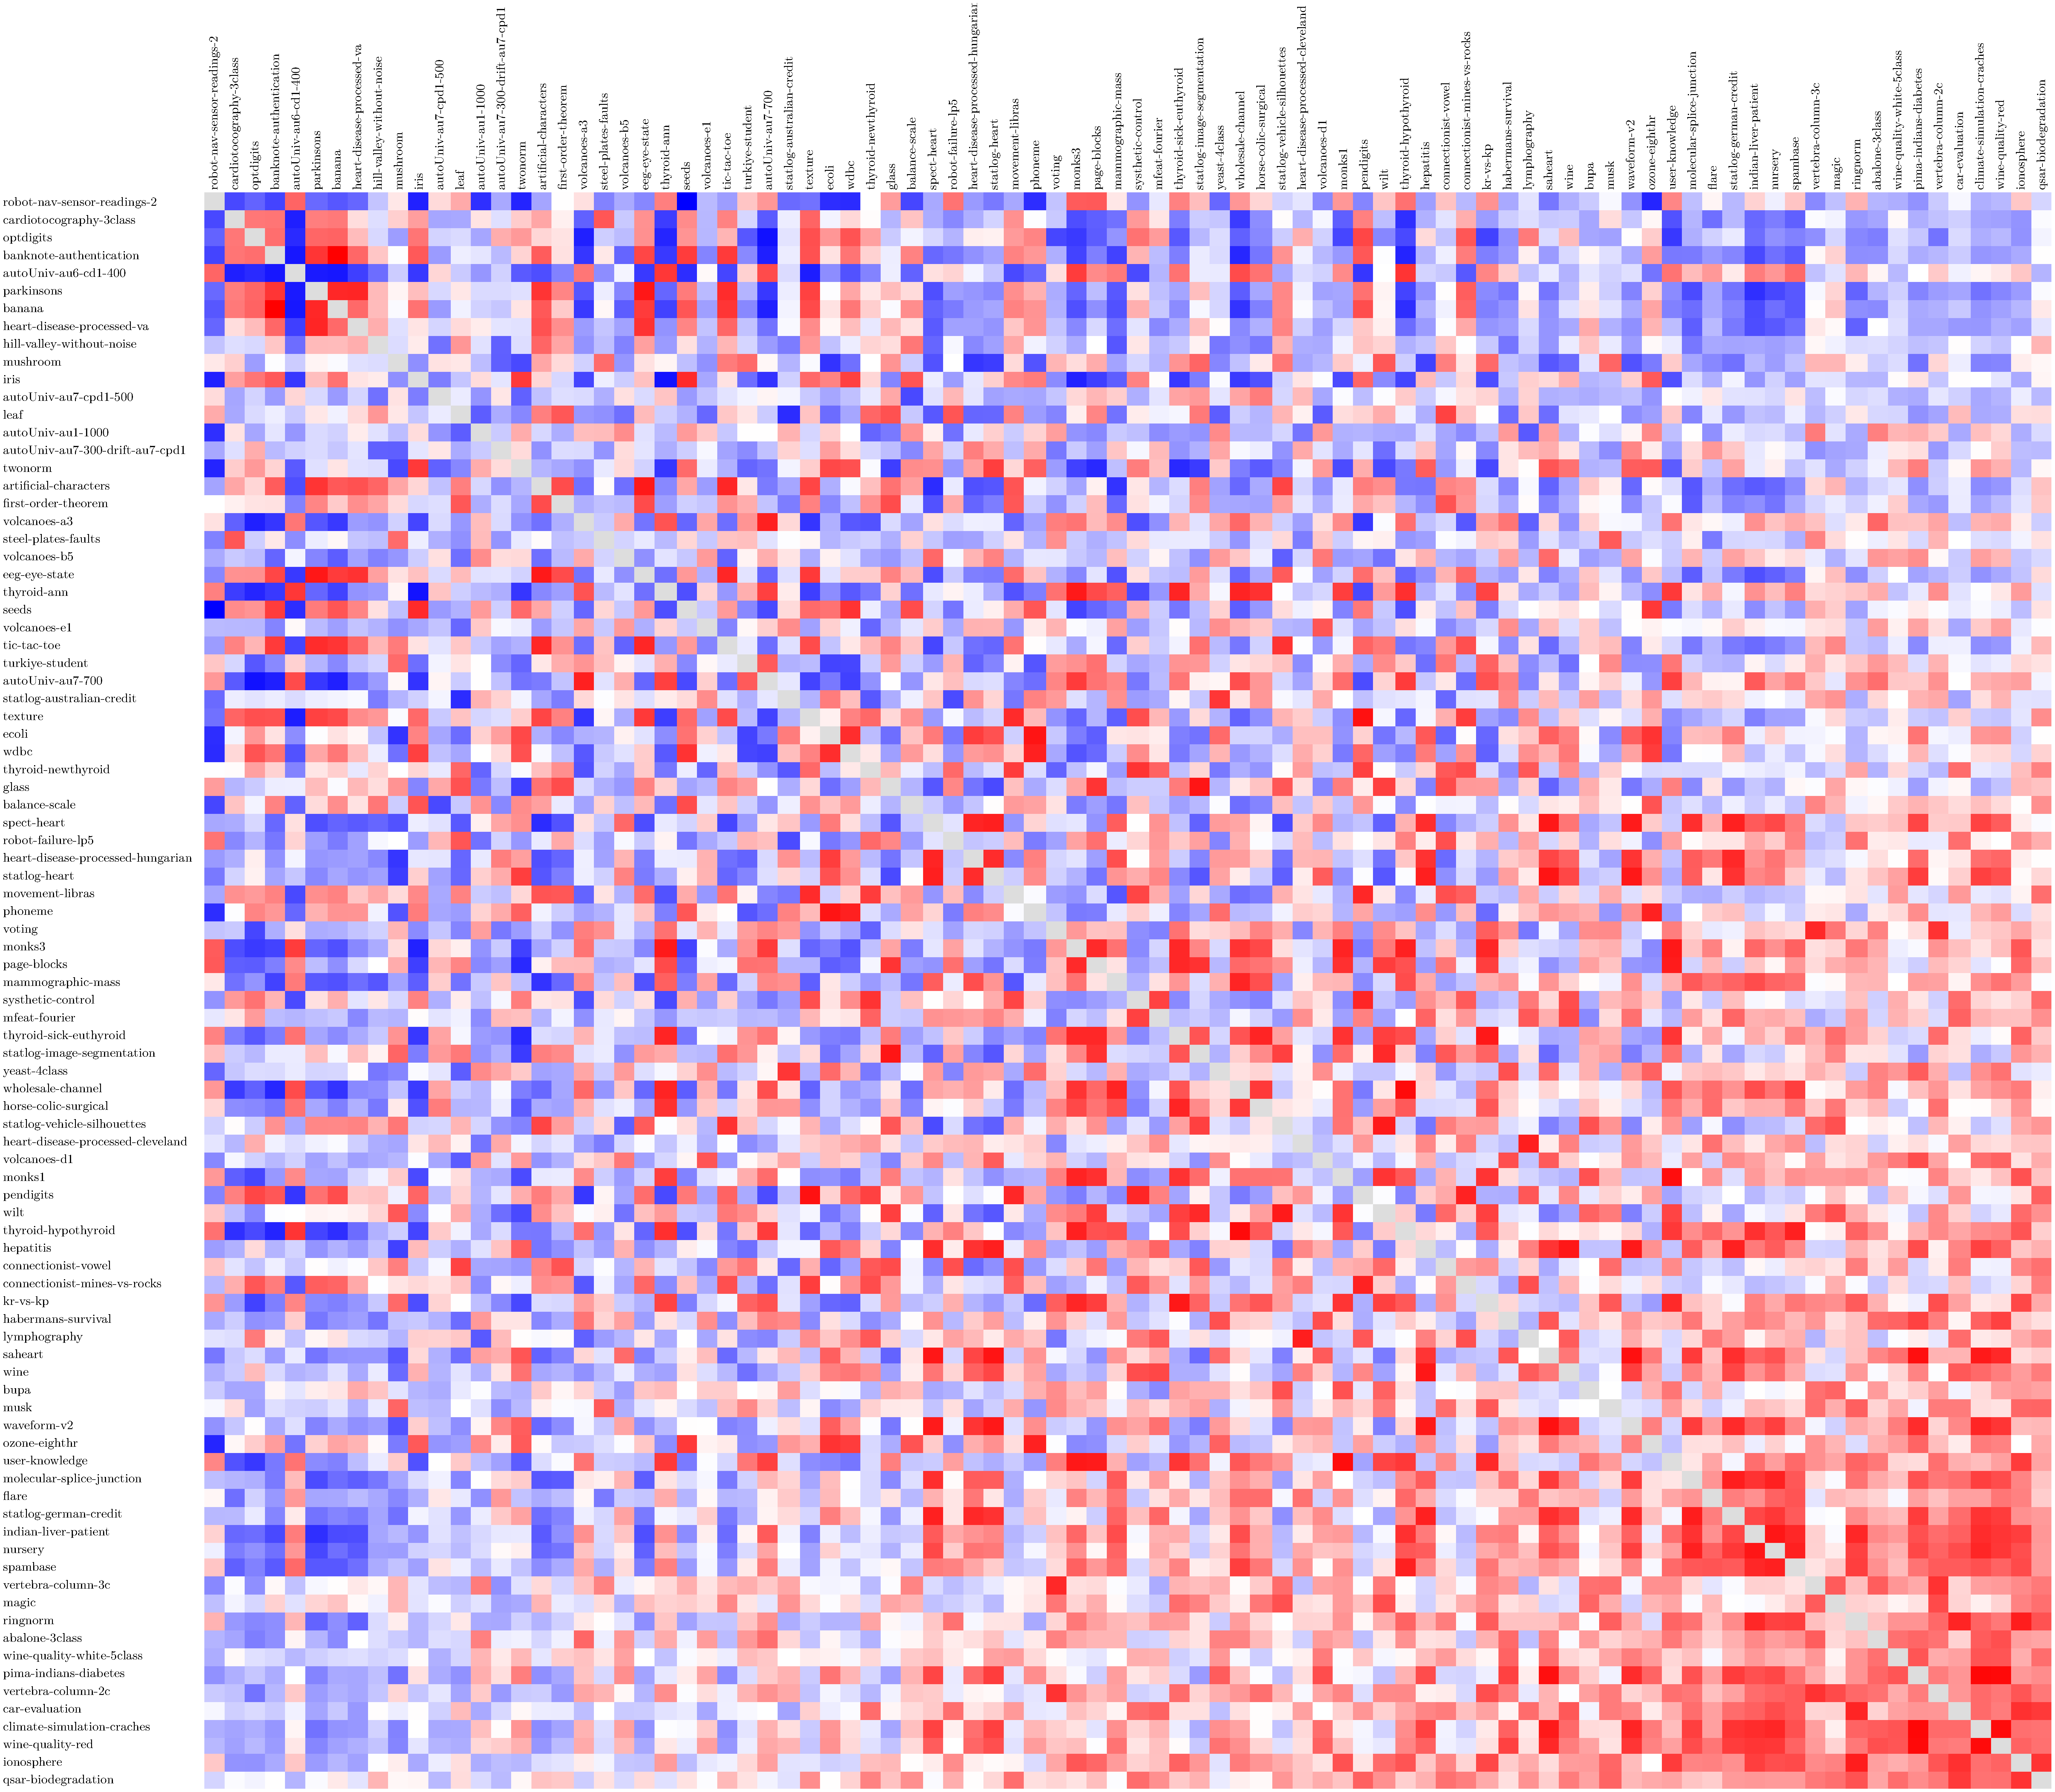
\includegraphics[scale=0.136]{images/heatbitmap.pdf}
  \caption[Correlação entre ranqueamentos de algoritmos de aprendizado.]{Visão geral da intensidade de correlação entre ranqueamentos de algoritmos de aprendizado para cada par possível na coleção. \textit{Azul: mais adequado. Vermelho: menos adequado.}}
  \label{datasetsimistodos}
\end{figure}
O mapa de calor com os valores de correlação dos conjuntos que apresentaram valores acima de $0,8$ é apresentado com maior clareza na Figura \ref{datasetsimis}.
\begin{landscape}
\begin{figure}
  \setlength{\unitlength}{1.0cm}
  \centering
    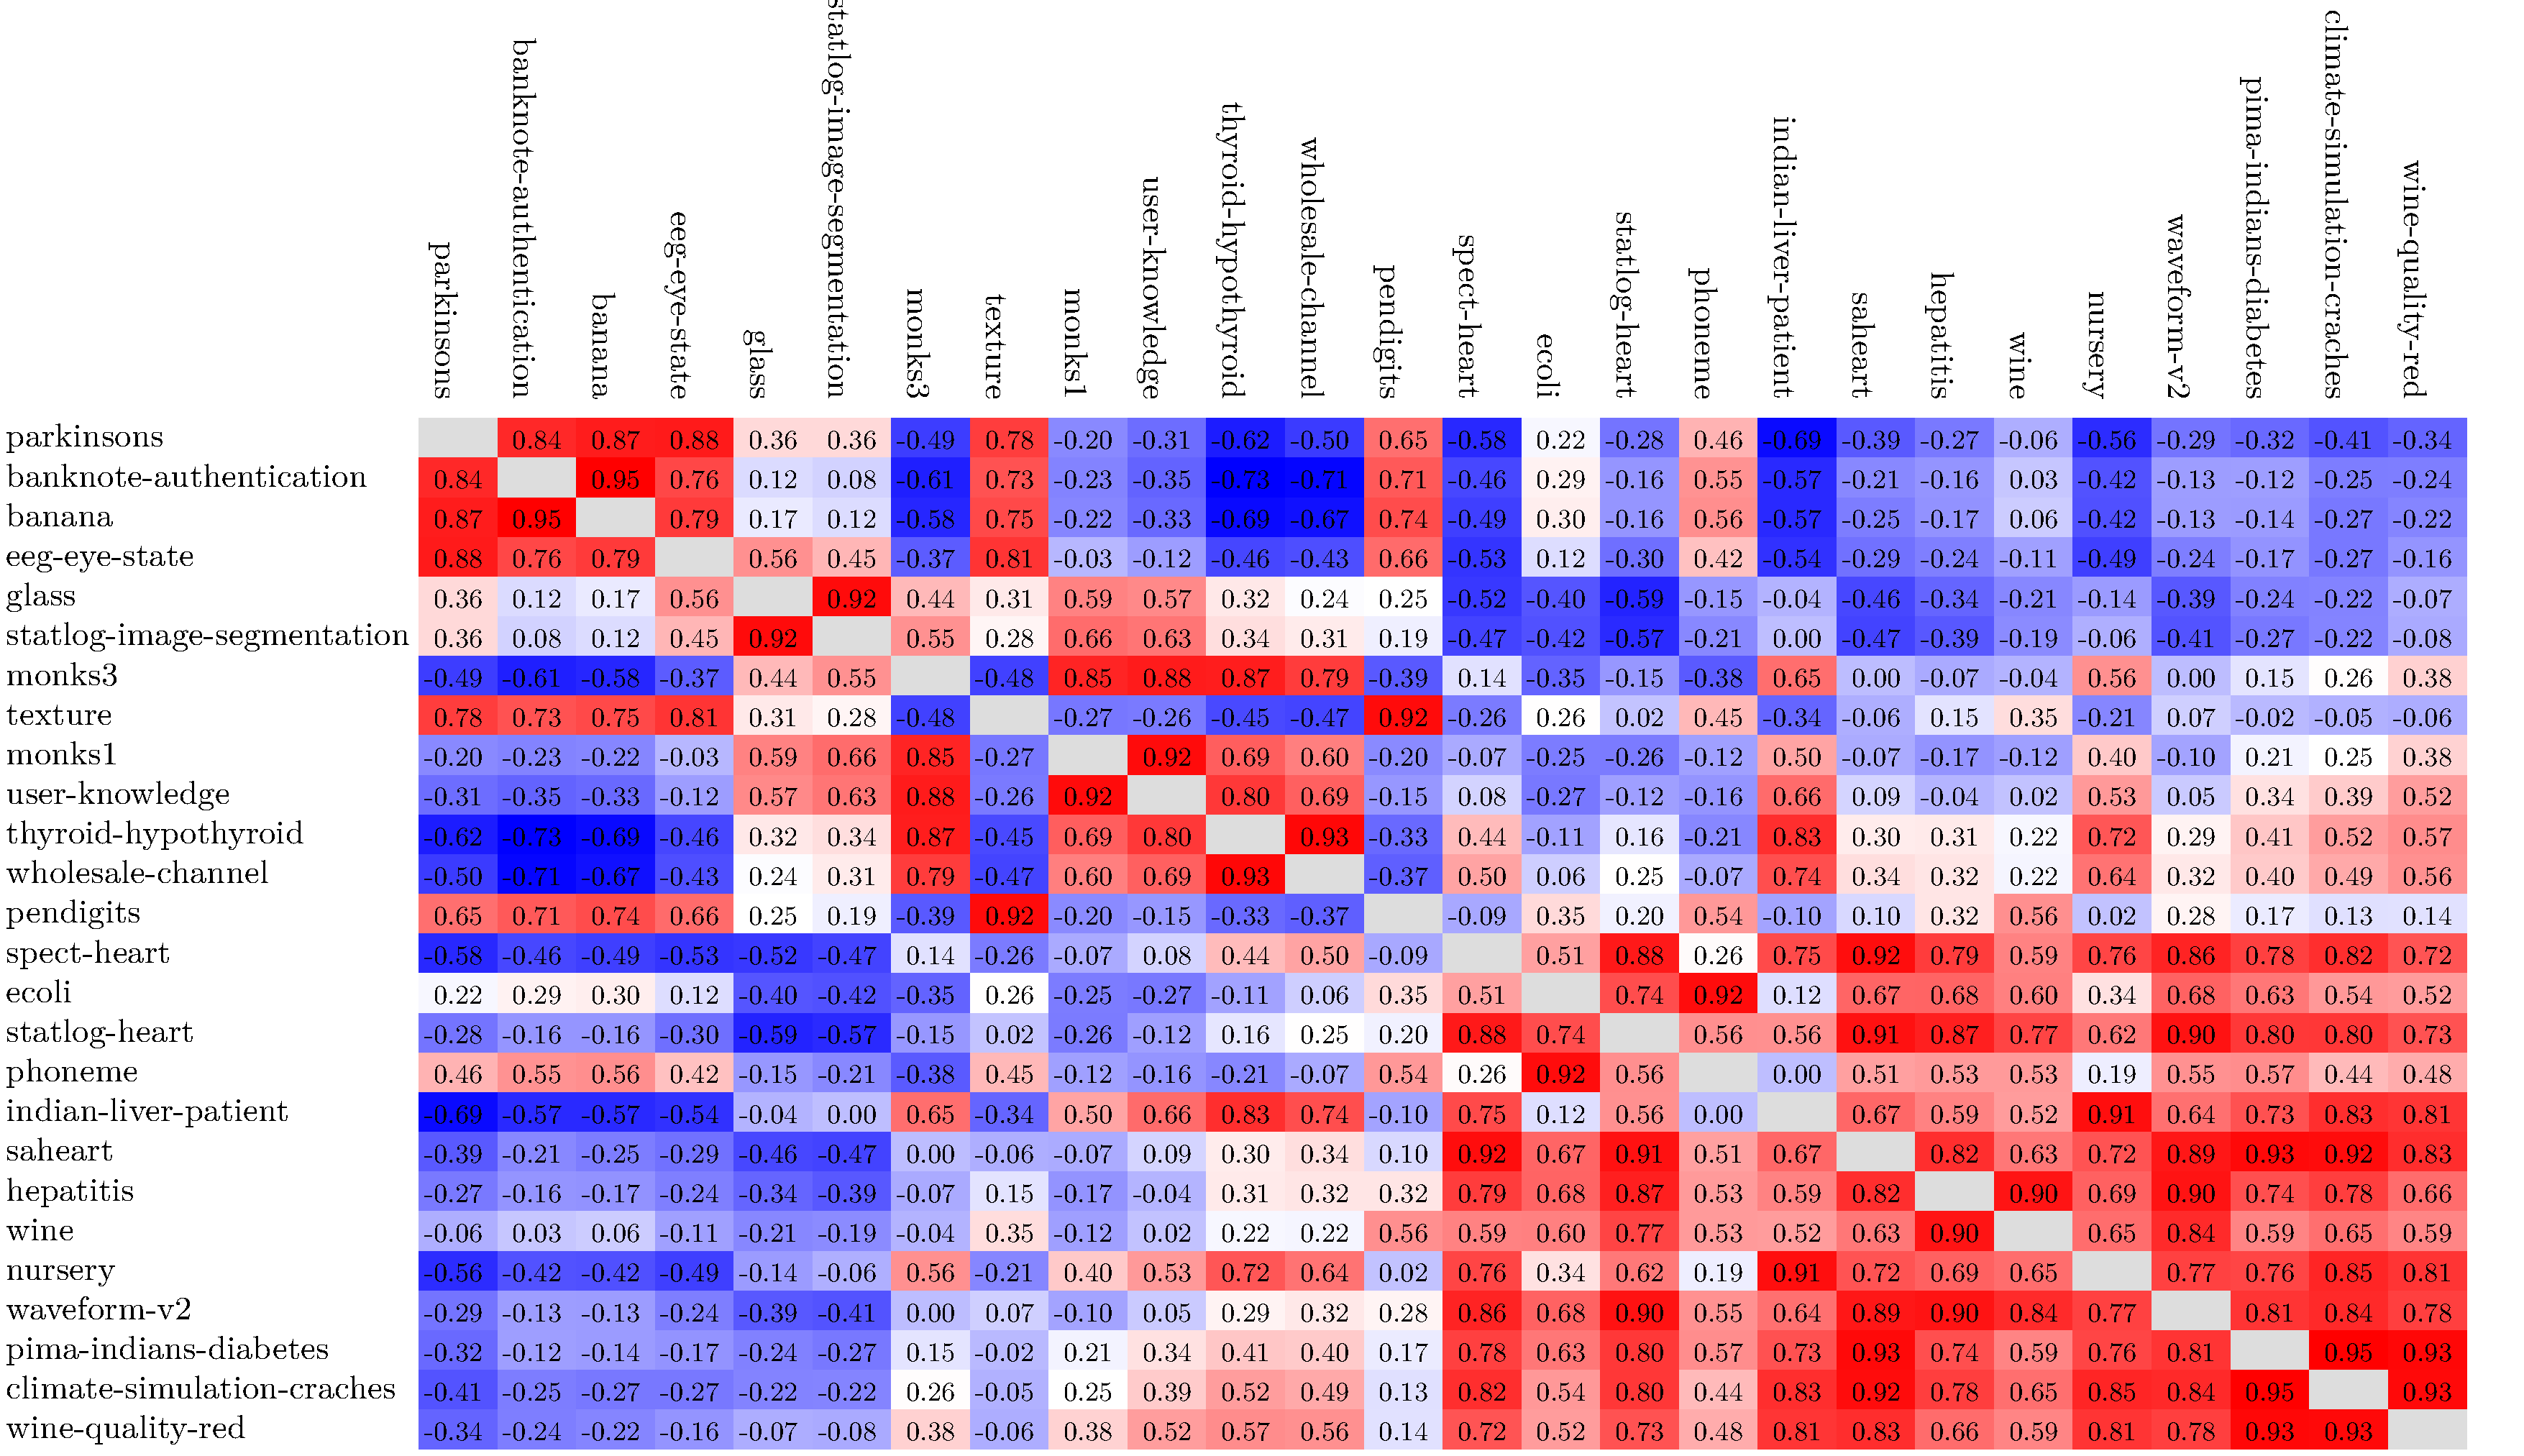
\includegraphics[scale=0.43]{images/heatmap-final-datasets.pdf}
  \caption[Valores de correlação entre conjuntos de dados mais correlacionados.]{
Valores de correlação entre os conjuntos de dados mais correlacionados.
}
  \label{datasetsimis}
\end{figure}
\end{landscape}
Variações como \textit{thyroid-sick-euthyroid} e \textit{thyroid-hypothyroid} ou \textit{volcanoes-d1} e \textit{volcanoes-e1} foram consideradas do mesmo domínio, porém como problemas distintos.
Na Tabela \ref{heatpares}, é possível observar que os domínios começam a coincidir somente com correlações abaixo de 0,830, havendo 18 pares de domínios distintos acima desse valor.
Logo, foi suposto que abaixo desse valor a coincidência de domínios fosse pouco preocupante.
Entretanto, análises posteriores ao término da presente pesquisa (Apêndice \ref{apflu}) indicam que seria fundamental manter apenas um conjunto de dados por domínio, para que a generalidade do aprendiz meta-ativo pudesse ser verificada.
\begin{table}
\caption[Pares de conjuntos com as maiores correlações.]{Pares de conjuntos com as maiores correlações. \textit{Pares em negrito relacionam conjuntos de domínios possivelmente próximos. Linha pontilhada simples indica omissão de pares de conjuntos de domínios distintos. Linha pontilhada dupla indica omissão de pares em geral.}}
\label{heatpares}
\centering\scalebox{0.842}{
\begin{tabular}{llr}
 \toprule
 \textbf{Primeiro conjunto} & \textbf{Segundo conjunto} &  \textbf{Correlação} \\
 \midrule
banana                             & banknote-authentication            & 0,950\\
climate-simulation-craches         & pima-indians-diabetes              & 0,949\\
pima-indians-diabetes              & wine-quality-red                   & 0,944\\
thyroid-hypothyroid                & wholesale-channel                  & 0,941\\
climate-simulation-craches         & wine-quality-red                   & 0,940\\
monks1                             & user-knowledge                     & 0,932\\
pima-indians-diabetes              & saheart                            & 0,926\\
saheart                            & waveform-v2                        & 0,924\\
pendigits                          & texture                            & 0,921\\
saheart                            & statlog-heart                      & 0,912\\
ecoli                              & phoneme                            & 0,912\\
glass                              & statlog-image-segmentation         & 0,909\\
indian-liver-patient               & nursery                            & 0,906\\
saheart                            & spect-heart                        & 0,903\\
eeg-eye-state                      & parkinsons                         & 0,903\\
hepatitis                          & wine                               & 0,902\\
monks3                             & user-knowledge                     & 0,900\\
statlog-heart                      & waveform-v2                        & 0,900\\
\textbf{thyroid-ann                        } & \textbf{thyroid-hypothyroid                }& 0,829\\ \hdashline
\textbf{vertebra-column-2c                 } & \textbf{vertebra-column-3c                 }& 0,821\\ \hdashline
\textbf{statlog-german-credit              } & \textbf{statlog-heart                      }& 0,821\\ \hdashline
\textbf{statlog-image-segmentation         } & \textbf{statlog-vehicle-silhouettes        }& 0,776\\ \hdashline
\textbf{autoUniv-au6-cd1               } & \textbf{autoUniv-au7-700                   }& 0,744\\ \hdashline
\textbf{thyroid-hypothyroid                } & \textbf{thyroid-sick-euthyroid             }& 0,740\\ \hdashline
\textbf{wine-quality-red                   } & \textbf{wine-quality-white-5class          }& 0,712\\ \hdashline
\textbf{volcanoes-d1                       } & \textbf{volcanoes-e1                       }& 0,712\\ \hdashline
\textbf{robot-failure-lp5                  } & \textbf{robot-nav-sensor-readings-2        }& 0,618\\ \hdashline
\textbf{volcanoes-b5                       } & \textbf{volcanoes-d1                       }& 0,606\\ \hdashline
\textbf{wine                               } & \textbf{wine-quality-red                   }& 0,590\\ \hdashline
\textbf{connectionist-mines-vs-rocks       } & \textbf{connectionist-vowel                }& 0,503\\ \hdashline
\textbf{volcanoes-b5                       } & \textbf{volcanoes-e1                       }& 0,500\\ \hdashline 
\hdashline
\textbf{autoUniv-au6-cd1-400               } & \textbf{autoUniv-au7-300-drift-au7,,,}& 0,000\\ \hdashline
\hdashline
\textbf{statlog-heart                      } & \textbf{statlog-image-segmentation         }& -0,524\\ \hdashline
robot-nav-sensor-readings-2        & seeds                              & -0,888\\
\bottomrule
\end{tabular}}
\end{table}

\subsection{Descrição}\label{descdatasets}
Todos os conjuntos selecionados, após particionamento dos dados durante o processo de validação cruzada, oferecem uma reserva com pelo menos 100 exemplos.
% $|\mathcal{U}|\geq 100$
Essa quantidade corresponde a um padrão de quantidade de consultas permitidas, de modo que as curvas de aprendizado de todos os conjuntos de dados sejam comparáveis entre si.
Os conjuntos têm suas características expostas no Apêndice \ref{apdatasets} - tabelas \ref{tab:datasetsa} e \ref{tab:datasetsb}.
Para ilustrar a diversidade dos conjuntos, alguns grupos especiais foram criados da seguinte forma:
\begin{itemize}
 \item classe majoritária 20 vezes mais numerosa que a classe minoritária (Tabela \ref{tab:imb});
 \item 60 ou mais atributos (Tabela \ref{tab:x});
 \item mais de 6 classes (Tabela \ref{tab:y});
 \item mais de 4000 exemplos (Tabela \ref{tab:n}); e,
 \item menos de 200 exemplos (Tabela \ref{tab:nm}). 
\end{itemize}

\input tex/dataset-tables-reduxes

Devido à presença de atributos nominais e numéricos, os algoritmos providos pela ferramenta Weka \cite{journals/sigkdd/HallFHPRW09} fizeram eventual uso de seus próprios filtros internos para lidar com cada tipo de atributo de acordo com a natureza do algoritmo: binarização, discretização e \ing{padronização}{z-score} \cite{kreyszig2007advanced}.
% Os algoritmos SVM e RoF (Seção \ref{learners}) requereram aplicação dos filtros externamente devido a incompatibilidade de seus filtros internos com alguns conjuntos de dados.

Exemplos duplicados foram removidos visando simular um oráculo consistente.
A cada grupo de exemplos repetidos, um único representante foi mantido cuja classe atribuída foi a moda das classes contempladas pelo grupo.

\section{Algoritmos de aprendizado}\label{learners}
Cada algoritmo de aprendizado tem, intrinsecamente, um viés próprio (Apêndice \ref{apmeta}) que, quando integrado a uma estratégia de amostragem ativa, pode influenciar no desempenho da estratégia.
Dessa forma, diferentes algoritmos foram adotados na comparação de estratégias.

As implementações adotadas são aquelas presentes na biblioteca Weka:
\sigla{\textit{k}-NN}{\textit{k}-vizinhos mais próximos}\footnote{Chamado IBk na implementação Weka.};
\sigla{C4.5w}{árvore de decisão C4.5}\footnote{Chamado J48 na implementação Weka.};
NB (\textit{Naive Bayes}); e,
\textit{Support Vector Machines} (SVM)\footnote{Invólucro LibSVM para Weka.}
\cite{journals/tit/Hart68,
books/mk/Quinlan93,
conf/ecml/Lewis98,
hearst1998support}.
O sufixo \textit{w} foi acrescentado como indicativo de que a implementação Weka não corresponde diretamente ao algoritmo original.

Algoritmos que requeiram ajuste externo de parâmetros frequentemente dependem de métodos de seleção de modelo \cite{arlot2010survey}.
Entretanto, no cenário de aprendizado ativo, o conjunto de treinamento é pequeno durante a maior parte da curva de aprendizado, tornando a seleção de modelos pouco confiável.
Adicionalmente, a complexidade dos métodos de seleção de modelo é computacionalmente incompatível com a necessidade de induzir um novo modelo a cada nova consulta.
Por fim, tendo em vista que o objetivo da seleção de algoritmos descrita nesta seção não foi a maximização da acurácia de algum algoritmo em particular, mas fornecer uma diversidade de vieses de aprendizado, não era mandatório que os parâmetros fossem otimamente ajustados.
Consequentemente, optou-se por valores pré-definidos.
O ajuste de parâmetros foi feito de acordo os valores padrão das implementações e as necessidades do aprendizado ativo, conforme listado a seguir.
\begin{itemize}
   \item \textit{k}-NN (denominado 5NN daqui em diante) - A quantidade adotada de 5 vizinhos possibilitou uma estimação de probabilidades com uma resolução que permite 6 valores quando todos os exemplos estão à mesma distância: 
   \[P_{\theta}(y|\bm{x}) \in \{0,0; 0,2; 0,4; 0,6; 0,8; 1,0\} \forall \bm{x} \in X, y \in Y\]
   Quanto maior a resolução, mais detalhada é a comparação de medidas de informatividade.
O voto de cada vizinho foi ponderado por $1 - d$ para atenuar as estimativas de probabilidade, onde $d$ é a distância euclidiana padronizada \cite{kreyszig2007advanced}.
\item C4.5w - A ramificação dos nós de decisão foi múltipla (não apenas binária), com fator de confiança na poda $0,25$ e % (smaller values incur more pruning)
um valor mínimo de 2 exemplos por folha.
A poda se deu com a \ing{substituição de nós por folhas}{subtree replacement}.
A estimação de probabilidades foi realizada com suavização aditiva \cite{books/daglib/0021593}, com o objetivo de atenuar as medidas de informatividade.
	\item NB - Uma discretização supervisionada de atributos numéricos foi realizada antes de cada treinamento \cite{conf/ijcai/FayyadI93}.
	\item SVM - Tipo C-SVC \cite{journals/ml/CortesV95} com núcleo função de base radial.
Os parâmetros, de acordo com a notação usual na literatura de SVM, seguiram os seguintes valores: $\gamma=0,5$;
% \item cache 200MB
% Shrinking(false)
% ProbabilityEstimates(true)
$C=1$; e, $\epsilon=0,001$ (tolerância do critério de parada). %SVMmulti eps=0,1

%inverse of the radius of influence of support vectors
% classif/learner g=0.5; SVMmulti g=1
%A low C makes the decision surface smooth, high C aims at classifying all training examples correctly
\end{itemize}

Um experimento envolvendo comitês também foi realizado.
Eles são apresentados na Seção \ref{algensembles}.

\subsection{Comitês}\label{algensembles}
Um comitê de classificadores é composto por diversos modelos visando um aumento na acurácia preditiva (Seção \ref{qbc}).
Um efeito colateral está na geração de estimativas de probabilidade mais tênues por serem baseadas na sumarização de predições feitas por modelos distintos e, em algum grau, independentes.
Estratégias de amostragem ativa baseadas na incerteza do modelo podem se beneficiar de predições atenuadas, pois elas podem aumentar seu poder discriminatório durante a comparação de exemplos para consulta.
Esse benefício é mais notável quando o algoritmo tende a gerar modelos excessivamente confiantes.
Segundo \citeonline{conf/icml/RoyM01}, o algoritmo NB, por exemplo, produz estimativas de probabilidade erroneamente elevadas para exemplos de fronteira quando sua premissa de independência entre os atributos é quebrada.
Uma solução proposta por esses autores é a adoção de um comitê do tipo \textit{bagging} (Seção \ref{qbc}).

Visando aumentar a abrangência dos resultados, optou-se, aqui, pela inclusão de um experimento com comitês.
Dois comitês equiparáveis e com desempenho geral elevado \cite{journals/jmlr/DelgadoCBA14} foram escolhidos: \sigla{RoF}{\textit{Rotation Forest}} e \sigla{RFw}{\textit{Random Forest}}
% Delgado: 121 datasets
\cite{journals/pami/RodriguezKA06,journals/ml/Breiman01}.
% RFw não realiza poda e faz a escolha aleatória de $\log_2|A| + 1$ atributos por árvore.
A escolha desses dois algoritmos permitiu a realização de um experimento com a acurácia preditiva num patamar superior à que foi obtida no experimento de modelos únicos.
Os comitês foram configurados com apenas 10 membros, devido às limitações de recursos computacionais anteriormente mencionadas (Seção \ref{sectempo}).

Nesta tese, comitês também foram aplicados a uma tarefa de regressão, que consistiu na predição de ranqueamentos pelo algoritmo \sigla{PCT}{\textit{Predictive Clustering Trees}} para o sistema de recomendação automática - introduzido na Seção \ref{algmeta}.

\subsection{Diversidade de algoritmos}
O mesmo procedimento experimental da Seção \ref{secsimi} foi adotado para avaliar a similaridade entre os algoritmos de aprendizado,
com exceção da medida de correlação, que foi substituída pela distância de Hamming \cite{hamming1950error}.
Essa métrica quantifica as predições distintas entre cada par de modelos para uma dada coleção de conjuntos de dados.
Ela representa diretamente o grau de equivalência entre algoritmos do ponto de vista da predição de classes.
Logo, é mais precisa que a medida anterior (Seção \ref{secsimi}).

O algoritmo 5NN foi testado com duas métricas de distância e com a opção de ponderação.
A versão com ponderação (indicada nesta seção pelo sufixo \textit{p}) foi preferida por permitir estimativas de probabilidade atenuadas, necessárias para parte das estratégias de amostragem ativa.
As versões com a distância de Manhattan (indicada pelo sufixo \textit{m}) foram descartadas devido à excessiva semelhança com as versões baseadas na distância euclidiana, pois obteve valores 0 e 13 no cálculo da distância de Hamming - conforme Figura \ref{leasimis}.
\begin{figure}
  \setlength{\unitlength}{1.0cm}
  \centering
    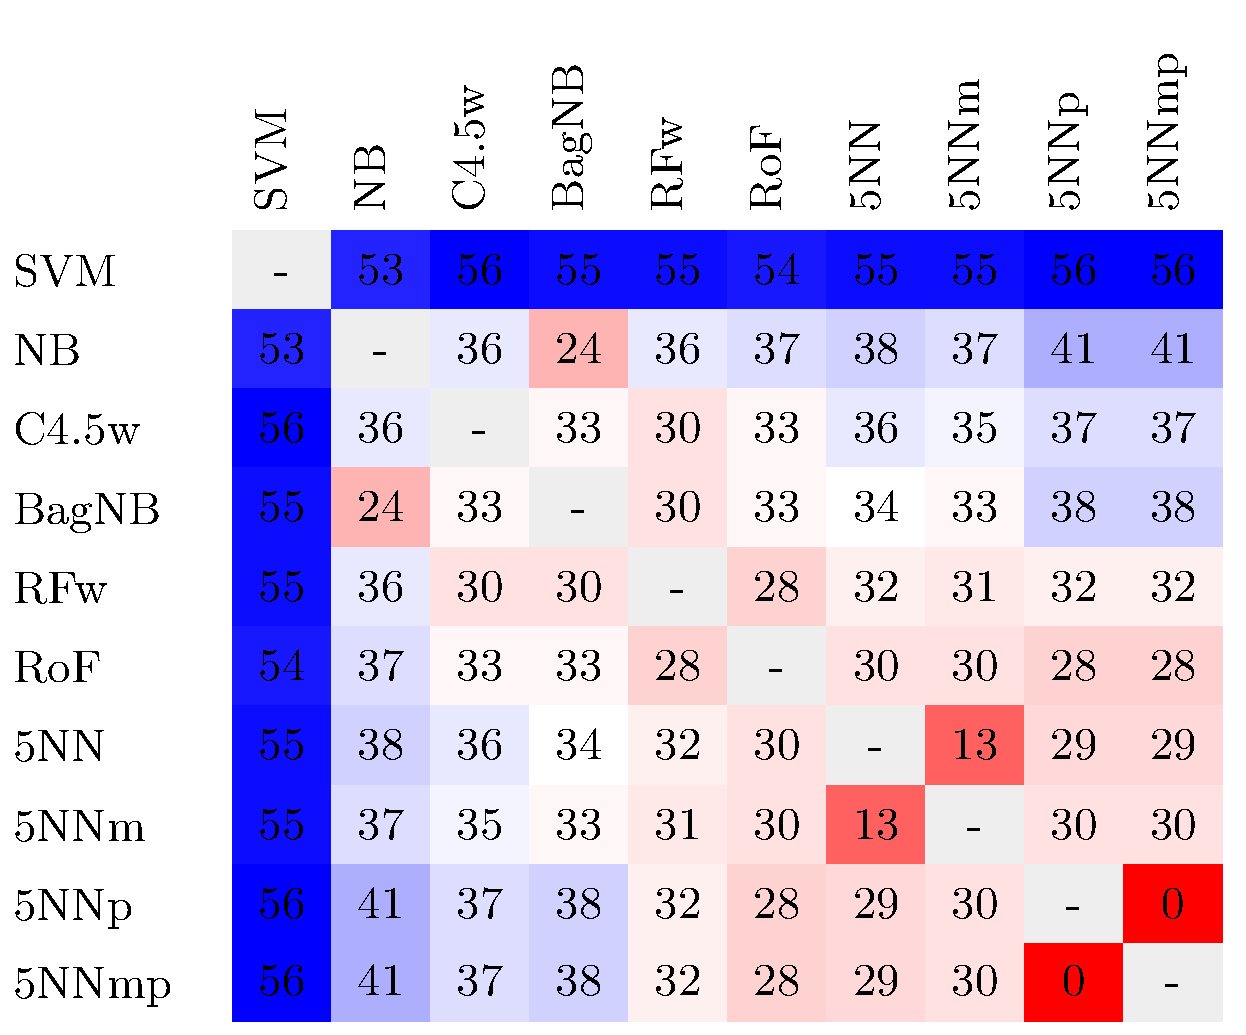
\includegraphics[scale=0.45]{images/heatmap-final-leas.pdf}
  \caption[Média da distância de Hamming entre predições de modelos induzidos]{Média da distância de Hamming entre as predições de modelos induzidos por diferentes algoritmos.}
  \label{leasimis}
\end{figure}



\subsection{Algoritmos de (meta) aprendizado}\label{algmeta}

É esperado que apenas parte dos 53 meta-atributos definidos na Seção \ref{sec:ama} seja relevante na tarefa de predição de ranqueamento ou recomendação de algoritmos.
Logo, os algoritmos de aprendizado mais apropriados são aqueles capazes de lidar com atributos irrelevantes.
Um tipo de algoritmo com essa capacidade frequentemente empregado é o comitê de árvores \cite{strobl2009introduction}.
Quatro algoritmos baseados em comitê de árvores com relatos de alto desempenho em geral \cite{journals/jmlr/DelgadoCBA14} frente a outros algoritmos são RFw, RoF (Seção \ref{algensembles}), \textit{Predictive Clustering Trees} (PCT) e, não necessariamente baseado em árvores, \sigla{ABoo}{AdaBoost} - \cite{journals/jmlr/DelgadoCBA14,conf/icml/FreundS96,conf/ecml/TodorovskiBD02}.
Eles foram adotados para gerar os modelos de recomendação do sistema de meta-aprendizado.
O prefixo \textit{meta} é acrescentado para desfazer qualquer ambiguidade entre o nível base e o nível meta - exemplos de uso: \ul{meta}PCT, EERent-\ul{meta}RoF, \ul{meta}-aprendiz, \ul{meta}classe, \ul{meta}exemplos, \ul{meta}conjunto de dados etc.

Optou-se pela quantidade padrão de 500 membros definido na implementação do algoritmo \textit{Random Forest} para a linguagem R \cite{team2014r}.
Esse número foi considerado válido pelos seguintes motivos:
\begin{itemize}
   \item é importante garantir que a quantidade de membros seja grande o bastante para não haver perda de acurácia devido a falta de membros - 128 árvores foram suficientes para atingir a acurácia máxima numa coleção de 29 conjuntos de dados, segundo \citeonline{conf/mldm/OshiroPB12};
%http://download.springer.com/static/pdf/998/chp%253A10.1007%252F978-3-642-31537-4_13.pdf?originUrl=http%3A%2F%2Flink.springer.com%2Fchapter%2F10.1007%2F978-3-642-31537-4_13&token2=exp=1446670434~acl=%2Fstatic%2Fpdf%2F998%2Fchp%25253A10.1007%25252F978-3-642-31537-4_13.pdf%3ForiginUrl%3Dhttp%253A%252F%252Flink.springer.com%252Fchapter%252F10.1007%252F978-3-642-31537-4_13*~hmac=d7f4c13c3879943df0e5b9f9f9fc8da7066cef8851e5fd261f98bee18f8a35c7
% as the number of trees grows, it does not always mean the performance of the forest is significantly better than previous forests (fewer trees), and doubling the number of trees is worthless. It is also possible to state there is a threshold beyond which there is no significant gain, unless a huge computational environment is available.
   \item o fator determinante na escolha do tamanho do comitê é o custo computacional \cite{conf/mldm/OshiroPB12};
   \item o risco de sobreajuste nesse parâmetro é baixo ou inexistente devido ao \textit{paradoxo da generalização do comitê} \cite{elder2003generalization,series/synthesis/2010Seni};
   \item é uma quantidade computacionalmente viável para o experimento do nível meta; e,
   \item sendo um número padrão, facilita a replicabilidade ou comparação com resultados de terceiros.
\end{itemize}

% A heurística de PCT para a definição de regras nos nós é a redução da variância.
%       "FTest = 1") ++
%       (if (ntrees == 1) Seq("PruningMethod = M5Multi", //ajuda C45 quebra
%         "M5PruningMult = 1", "")
%       else Seq("")) ++ //ajuda mais
        
\section{Estratégias}\label{confstrats}

Nos experimentos realizados, 9 estratégias e 5 variantes foram avaliadas.
O conjunto de estratégias selecionadas foi considerado representativo da diversidade de paradigmas relevantes de aprendizado ativo, de acordo com os artigos referenciados por \citeonline{series/synthesis/2012Settles}.

Foram acrescentados os sufixos \textit{euc} e \textit{man} nas siglas de estratégias que façam uso das distâncias euclidiana e de Manhattan, respectivamente.
Os sufixos \textit{ent} e \textit{acu} indicam, respectivamente, os critérios de entropia e de acurácia balanceada para a estratégia EER (baseada na \textit{redução do erro esperado}).
Dentre as possibilidades iniciais, três estratégias foram descartadas.
SVMsim e SVMbal foram implementadas (Seção \ref{outras}), mas descartadas dada a sua dependência de um algoritmo específico e seu desempenho excessivamente baixo em testes iniciais - possivelmente devido a um insucesso da adaptação multiclasse escolhida.
QBC (\textit{Query By Committee}) foi implementada para o comitê RFw com a medida $\JS$ (Seção \ref{outras}), mas também descartada pelos mesmos motivos.
% journals/jmlr/BaramEL04 foram adaptados para contemplar problemas multiclasse por meio da aplicação de \ing{rodízio}{round-robin} entre sub-estratégias. A cada sub-estratégia foi atribuída uma classe principal na configuração \textit{um para muitos}.

Um conjunto reduzido de estratégias foi utilizado na parte inicial da análise comparativa (Seção \ref{despred}).
Assim, somente uma variante por estratégia foi selecionada para esse primeiro momento.
As variantes não incluídas foram as seguintes:
\begin{itemize}
%    \item DW (DWeuc e DWman) \ano{sigla} - DW é conceitualmente e experimentalmente inferior a TU \cite{bracis15}, cujo paradigma \ano{termo} a representa parcialmente;
   \item ATUman, DWman, TUman e HTUman (todas as estratégias baseadas em densidade) - a distância euclidiana foi considerada mais usual que a distância de Manhattan, cujo desempenho, em geral, é similar \cite{bracis15}; e,
   \item EERacu - a variante EERent foi preferida porque $E$ (entropia) é a medida proposta no trabalho original.
\end{itemize}

Algumas das estratégias exigiram configurações específicas.
As escolhas adotadas nessas configurações são detalhadas nas seções seguintes.

\subsection{EERent e EERacu} \label{eerconfig}
A utilização da acurácia balanceada \cite{journals/bmcbi/MassoV10} como função objetivo alternativa configurou-se como uma variação do método (EERacu), visando agir diretamente na medida de interesse nos experimentos (Seção \ref{medidas}).
A acurácia balanceada foi preferida à $\kappa$ por ser uma medida multiclasse com menos propensão a ter valores próximos ou iguais a zero, evitando, assim, o anulamento da medida de informatividade.
Apenas 100 exemplos foram aleatoriamente amostrados de $\mathcal{U}$ antes de cada consulta para reduzir o alto custo computacional de EER.

\subsection{HS}\label{metohs}
A implementação original do autor foi empregada neste trabalho com o mesmo
algoritmo de agrupamento, 
\textit{Ward's average linkage method}\footnote{
Implementação disponível no Weka \cite{journals/sigkdd/HallFHPRW09}.}.

\subsection{DW, TU, ATU e HTU}
Os parâmetros de ponderação foram fixados no valor 1 ($\alpha=1$, $\delta=1$).

\section{Avaliação}\label{avaliacao}
A avaliação dos resultados experimentais foi realizada qualitativamente por meio de curvas de aprendizado e quantitativamente por meio de medidas de desempenho (Seção \ref{medidas}).
As formas de validação são apresentadas na Seção \ref{validacao}.
A parte quantitativa foi confirmada por testes estatísticos (seções \ref{testestbase} e \ref{testestmeta}). 

\subsection{Medidas}\label{medidas}
Nos experimentos desta tese, foram necessárias medidas de avaliação de desempenho preditivo específicas para o nível base e para o nível meta.
Essas medidas são apresentadas nas seções seguintes.

\subsubsection{Nível base}\label{metrbase}
\simbolo{\mu_\kappa}{valor médio de $\kappa$ para 5 execuções de validação cruzada em 5 partes}
\simbolo{\sigma_\kappa}{desvio padrão de $\kappa$ para 5 execuções de validação cruzada em 5 partes}
% Settles (com f-measure e sem log(x))
% An analysis of active learning strategies for sequence labeling tasks (2008)
% No "active chalenge 2011", que alguns adotam como referência para citar ALC, foi usada a AUC verdadeira e log2(x) no cálculo (igual ao Cawley):
% http://www.causality.inf.ethz.ch/activelearning.php?page=evaluation
% Porém, eles avaliam sem validação cruzada, talvez por limitação do próprio fato de ser uma competição.
% O dataset inteiro é usado uma só vez e o teste é feito em cima de
% "all the samples with unknown labels".
% Isso explica o fato de classificadores semisupervisionados terem alavancado as estratégias na competição.

Uma medida de desempenho preditivo comumente utilizada na área de aprendizado ativo é a \ing{\sigla{ALC}{área debaixo da curva de aprendizado}}{Area under the Learning Curve}.
Uma das primeiras menções a esse tipo de medida em aprendizado ativo, até onde o conhecimento do autor permite dizer, foi feita por \citeonline{raghavan2007will}.
A medida ALC foi empregada em diversos artigos, como no trabalho de \citeonline{conf/emnlp/SettlesC08} e aplicado em momentos relevantes, como na competição de aprendizado ativo mencionada no Capítulo \ref{intro}.

A ALC é o valor resultante do somatório de alguma medida de desempenho ao longo das consultas.
Seu intuito é avaliar o desempenho geral de uma estratégia, ou seja, em uma ampla faixa de orçamentos.
Logo, a medida se mostra adequada para os objetivos desta tese, relacionados à comparação de estratégias.
Neste trabalho, ela foi adotada em conjunto com a extensão do índice kappa de Cohen, $\kappa$ - detalhada na Seção \ref{newhtu}.
Na descrição dos resultados, os valores de ALC apresentados são o resultado da divisão da ALC pela quantidade de consultas, visando manter a interpretabilidade da medida.

O índice $\kappa$ é utilizado para comparar o grau de consenso entre avaliadores \cite{journals/coling/EugenioG04}.
Seu poder discriminatório tem sido satisfatório frente a outras medidas de sumarização da matriz de confusão \cite{conf/acivs/DemirkesenC08}.
Quando aplicado como medida de desempenho de classificação, o valor limite $1$ indica acerto total, $0$ desempenho equivalente ao aleatório e $-1$ erro total. Entretanto, nem sempre o limite inferior coincide com $-1$ \cite{journals/ese/Emam99}.
Esse índice permite realizar a comparação sob dois pontos de vista: entre estratégias (valor relativo) e em relação ao acaso (valor absoluto).

Dada a presença de um alto grau de desbalanceamento entre as classes nos conjuntos de dados da coleção, a medida de acurácia convencional seria uma medida de desempenho inadequada, pois permitiria que a classe majoritária dominasse a composição de seu valor final.
De fato, as proporções das classes majoritária e minoritária chegam a extremos de, respectivamente, $96,5\%$ e $0,0\%$ (1 exemplo) do tamanho da reserva - conforme Tabela \ref{tab:imb}.

As curvas de aprendizado e valores de ALC são baseadas nas médias das curvas resultantes de um procedimento de validação cruzada \cite{settles2010active}.
Cada curva exibe a medida de interesse $\kappa$ em função da quantidade de consultas.
Assim, neste texto,  o valor médio $\mu_{\kappa}$ de $\kappa$ para as 5 execuções de validação cruzada em 5 partes (Seção \ref{validacao}) é a medida base de todos os resultados sobre desempenho relacionado à capacidade preditiva.
%neste documento.
Como consequência, cada conjunto de dados tem um valor de $\mu_{\kappa}$ e seu correspondente desvio padrão $\sigma_{\kappa}$ para cada consulta de uma dada estratégia.
É importante diferenciar $\mu_{\kappa}$ (e $\sigma_{\kappa}$), que é uma média de valores $\kappa$ interna a cada conjunto de dados, da \textit{média de} $\mu_{\kappa}$ (e \textit{média de} $\sigma_{\kappa}$), que é calculada para a coleção como um todo.
% Logo, referências à \textit{média de} $\bar{\kappa}$ e ao \textit{desvio padrão de} $\bar{\kappa}$ indicam as estatísticas sobre $\bar{\kappa}$ em relação a todos os 90 conjuntos de dados.

\subsubsection{Nível meta}\label{avmeta}
A avaliação do sistema de recomendação foi realizada conforme dois cenários:
classificação 
% (metaestratégia/recomendação do melhor algoritmo)
e predição de ranqueamento de algoritmos.
% (estimação da colocação de cada candidato).
Seguindo a escolha de \citeonline{conf/ijcnn/SoutoPSACLS08}, a predição pelo \sigla{Def}{ranqueamento médio} foi uma das referências utilizadas na avaliação do sistema de recomendação.
O \sigla{Alea}{ranqueamento aleatório} e a \sigla{Maj}{escolha fixada na classe majoritária} também serviram de referência.
A comparação entre as predições de ranqueamento foi feita por meio do cálculo do coeficiente de correlação de Spearman (Seção \ref{secsimi}).
O desempenho de classificação foi avaliado pela comparação da medida $\kappa$ e, paralelamente, pelas acurácias ordinária e balanceada na predição de melhor algoritmo de aprendizado.
O mesmo método experimental foi adotado na investigação inicial de outras possibilidades de recomendação: de estratégias de amostragem ativa, de pares estratégia-algoritmo, de métricas de distância para estratégias baseadas em densidade e da própria utilização ou não de aprendizado ativo.

Para verificação da efetividade do sistema de recomendação, o efeito do meta-aprendiz também foi avaliado no nível base.
O algoritmo para o papel de aprendiz para cada dada estratégia foi escolhido automaticamente e seu desempenho foi comparado diretamente com os demais algoritmos no nível base por meio dos valores de ALC e curvas de aprendizado.

\subsection{Validação}\label{validacao}
Não há consenso na literatura de aprendizado ativo sobre a melhor maneira de validação.
% Uma consulta por ``cross-validation'' e ``active learning'' no google scholar em 12/10/15 retornou parte dos seguintes resultados mais referenciados diretamente relacionados à presente pesquisa.
Dados os recursos disponíveis, optou-se por 5 execuções de validação cruzada em 5 partes.
Ela tem uma menor variabilidade quando comparada à \sigla{LOO}{\textit{Leave-One-Out}} e à validação em 10 partes \cite{journals/neco/KearnsR99} e um menor enviesamento quando comparada, por exemplo, com a validação em 2 partes ou \textit{hold-out} \cite{arlot2010survey}.
Adicionalmente, a validação em 5 partes é uma configuração comum na literatura.
Algumas das possibilidades encontradas em trabalhos relevantes são as seguintes:
\begin{itemize}
 \item validação em conjunto à parte pré-definido pelos autores dos conjuntos de dados \cite{conf/cikm/ErtekinHBG07};
 \item 100 execuções de validação em conjunto com 40\% dos exemplos à parte \cite{journals/jmlr/BaramEL04}; % For almost all problems, this collection includes 100 folds each consisting of a fixed 60\%/40\% training/test partition.
 \item validação cruzada em 5 partes \cite{chen2015study,settles2008active,conf/ecml/LomaskyBAWF07,conf/ecir/XuAZ07}; % we used a 5-fold CV to assess accuracy. % we pursue 5-fold cross-validation on the Active-RDD algorithm and Gapped Top K algorithm, and compare their cross-validation performance (CVP) with Cluster Centroid and Top K algorithm performance,(these algorithms are consequently parameter free in this setting). We separate 50 queries into 5 parts, where each part contains 10 queries. For the kth set of queries, we train parameters to optimize the retrieval performance for the other 4 sets of queries, and use this set of the parameters to test on kth set of queries to obtain the retrieval performance measure for kth part. We do this for k = 1, 2, 3, 4, 5 and the cross-validation performance is the average performance on the 5 test query sets. The cross-validation experimental results are shown in Table 2.   
 \item 4 execuções de validação cruzada em 5 partes \cite{conf/ijcai/BeckerO05,conf/icml/MusleaMK02}; % We report the average over a 5-fold cross-validation to ensure statistical significance of the results. In a single fold, we randomly sample (without replacement) an initial labelled training set of a fixed size – 500 or 2,000 sentences, depending on the experiment – and a test set of 1,000 sentences. The remaining sentences constitute the global pool of unlabelled sentences (ca. 37,000 sentences) % four runs of 5-fold cross-validation.
 \item validação cruzada em 9 partes \cite{conf/iswc/StikicLS08}; % As suggested in [12], we use 9-fold leave-one-day-out cross validation on the data to avoid over-fitting. In each cross validation round of supervised learning, we train the algorithms on 8 days of data. In case of semi-supervised and active learning, only a subset of 2 days of data is used as an initial labeled training set. The algorithms are always tested on the left out day’s data.
 \item validação cruzada em 10 partes \cite{settles2008active}; % baselines: the cost-sensitive method using known annotation times, and random sampling. The task-models are evaluated with the F1 measure and averaged using ten-fold cross-validation (five-fold for CKB).
 \item 2 execuções de validação cruzada em 10 partes \cite{conf/ecml/KornerW06,conf/icml/MelvilleM04}; e,% We initiated the active learners with 50 randomly drawn training instances and evaluated the experiments based on 2x10-fold cross validation. During each iteration we added 1 query to the training set and proceeded until all available data was used or a maximum of 250 queries. 
 \item validação cruzada em 20 partes \cite{conf/ijcai/MusleaMK03}. % we use 20-fold cross-validation to compare the performance 
\end{itemize}

No nível meta, LOO foi utilizada na avaliação do desempenho na predição de ranqueamentos conforme sugerido por \citeonline{journals/ml/BrazdilSC03}.
Essa abordagem maximizou a utilidade dos dados disponíveis, que correspondem a apenas 90 metaexemplos, um para cada conjunto de dados.
Além disso, LOO fornece a estimativa menos enviesada da acurácia quando comparada às demais formas de validação cruzada \cite{conf/icml/Joachims00} e, nesse contexto, permite a aplicação de teste estatístico, conforme discutido na Seção \ref{testestmeta}.

Por outro lado, no caso da avaliação do desempenho de classificação no nível meta, o teste estatístico não pôde ser aplicado com confiabilidade pelos motivos descritos na Seção \ref{testestmeta}.
Optou-se, então, por dez execuções de validação cruzada em dez partes \cite{conf/pakdd/BouckaertF04}, 

% A survey of cross-validation procedures for model selection (2010):
% http://www.di.ens.fr/willow/pdfs/2010_Arlot_Celisse_SS.pdf
% …
% As noticed in the early 30s by Larson (1931), training an algorithm and evaluating its statistical performance on the same data yields an overoptimistic result.
% CV was raised to fix this issue, starting from the remark that testing the output of the algorithm on new data would yield a good estimate of its performance(Mosteller and Tukey, 1968; Stone, 1974; Geisser, 1975).
% …
% Leave-one-out (LOO, Stone, 1974; Allen, 1974; Geisser, 1975) is the most classical exhaustive CV procedure.
% …
% LOO bootstrap and .632 bootstrap. … these procedures have nearly no theoretical justification and only empirical studies have supported the good behaviour of .632+ bootstrap
% 
% tem até review de fast CVs.
% ;;;
% PASSIVO: According to Breiman and Spector (1992) the best risk estimator is LOO,
% whereas 10-fold CV is more accurate for model selection.
% }

\subsection{Teste estatístico no nível base}\label{testestbase}
% from cerri: Para verificar a significância estatística dos resultados, foram empregados os testes de Friedman e Nemenyi, recomendados para comparações envolvendo vários métodos e muitos conjuntos de dados (Demšar, 2006). O teste de Friedman é um teste não paramétrico, pois não assume nada acerca da distribuição dos dados. Ele é baseado em rankings, e verifica se há diferença estatisticamente significante em um grupo de comparações. O teste de Nemenyi é um teste post-hoc aplicado após o teste de Friedman. Ele é utilizado para encontrar quais pares de comparações apresentam diferenças estatisticamente significantes. Nos testes estatísticos, foi utilizado um nível de confiança de 95%.
As diferenças de desempenho preditivo foram atestadas pelo teste não paramétrico de Friedman com teste post-hoc de Nemenyi seguindo a abordagem proposta por \citeonline{journals/jmlr/Demsar06} para comparações de classificadores.
Ainda conforme a abordagem do autor daquele estudo, os valores foram arredondados na terceira casa decimal, para forçar o empate nas diferenças irrelevantes.
Os resultados do teste são sumarizados numa tabela cujas células contêm símbolos que indicam com que nível de significância estatística uma estratégia na linha vence a outra na coluna.
No exemplo com algoritmos hipotéticos dado na Tabela \ref{exfried}, o algoritmo 1 vence o algoritmo 2 com $p\valor<0,01$; o algoritmo 2 vence o algoritmo 3 com $p\valor<0,05$ e o algoritmo 3 vence o algoritmo 4 com $p\valor<0,10$.
A contagem de ocorrências de primeiros e últimos lugares é apresentada na Tabela \ref{exconta}.
\begin{table}
\parbox[t][]{.48\linewidth}{\vspace{0pt}
	\flushright
	\caption[Exemplo com legenda das diferenças estatisticamente significativas.]{Exemplo de tabela de sumarização de diferenças estatisticamente significativas.
	\textit{Cada símbolo representa um nível de significância estatística $\alpha$:}
	* ($\alpha=0,01$), + ($\alpha=0,05$) e . ($\alpha=0,10$).}
	\label{exfried}
	\scalebox{0.9}{
	\begin{tabular}{lccccc}
	\toprule
						& 1 & 2 & 3 & 4 & 5 \\[4pt] \midrule
		1 - algoritmo 1	& - & * &   &   &   \\[4pt]
		2 - algoritmo 2	&   & - & + &   &   \\[4pt]
		3 - algoritmo 3 & 	&   & - & . &   \\[4pt]
		4 - algoritmo 4	&   &   &   & - &   \\[4pt]
		5 - algoritmo 5 & 	&   &   &   & - \\\bottomrule
	\end{tabular}
	}
}
\hfill
\parbox[t][]{.48\linewidth}{\vspace{0pt}
	\flushright
	\caption[Exemplo de contagem de colocações.]{Exemplo de contagem de colocações. Medida: ALC-$\sigma_{\kappa}$. \textit{O melhor e o pior valor de cada coluna estão em \textcolor{blue}{\textbf{negrito azul}} e \textcolor{red}{\textbf{negrito vermelho}} respectivamente. Apenas negrito indica segundo melhor valor.}}
	\label{exconta}
	\scalebox{0.9}{
	\begin{tabular}{lccc}
		\toprule
		 &\scriptsize \makecell{\textbf{Primeiras}\\\textbf{colocações}} &\scriptsize \makecell{\textbf{Últimas}\\\textbf{colocações}} \\
		\midrule              
		algoritmo 1& \bom{78} & \bom{13} \\
		algoritmo 2& \bomd{67} & \ruim{91} \\
		algoritmo 3& 55 & \bomd{24} \\
		algoritmo 4& 43 & 44 \\
		algoritmo 5& \ruim{35} & 44 \\
	\bottomrule
	\end{tabular}
	}
}
\end{table}
O critério de vitória é baseado na comparação dos valores de ALC de $\mu_{\kappa}$ (ALC-$\mu_{\kappa}$) para os dois algoritmos em questão em cada conjunto de dados.


\subsection{Teste estatístico no nível meta}\label{testestmeta}
% Dá quase pra deduzir da Nathalie que é possível aplicar Friedman em um só dataset sem quebrar (muito) as premissas.
% Mas isso não chega a ter o peso de uma prescrição. De qualquer forma, o conjunto é pequeno demais para isso (9 exemplos, se k=10).
As diferenças estatisticamente significativas entre metaPCT e Def foram reveladas pelo teste de Wilcoxon pareado \cite{journals/jmlr/Demsar06} aplicado aos valores de correlação entre os ranqueamentos esperados e seus correspondentes ranqueamentos preditos (Seção \ref{avmeta}).
Cada metaexemplo representa um conjunto de dados.
Logo, houve uma aproximação da premissa de \textit{independência entre amostras} devido ao isolamento de cada metaexemplo sob teste - situação intrínseca ao procedimento LOO.
Assim, a avaliação da predição de ranqueamento está estatisticamente fundamentada.

Por outro lado, a comparação de acurácias entre múltiplos metaclassificadores não permite aplicar um teste estatístico baseado em ranqueamento, quando há um único metaexemplo no conjunto de teste.
O motivo dessa impossibilidade é o valor da predição de classe ser discreto e, consequentemente, só poder ser avaliado como correto ou incorreto.
Outras coleções de conjuntos de dados precisariam ser incorporadas ao experimento,
mas isso não é viável com a presente disponibilidade de conjuntos pré-processados.
Entretanto, é possível obter valores informativos do metaconjunto que representa a única coleção disponível, caso seja alterada a forma de validação cruzada.
A média e o desvio padrão do desempenho preditivo podem ser obtidos por meio de dez execuções de validação cruzada em dez partes.

A troca da forma de validação é preferível, pois o desvio padrão retornado por LOO seria desprovido de significado prático.
Ele teria um valor elevado que refletiria o fato dele ser fruto do caso extremo em que o conjunto de teste tem apenas um elemento.
Além disso, quando há apenas um conjunto de dados e uma única execução, o desvio padrão obtido por LOO é mera função direta da acurácia.
Isso pode ser verificado no desenvolvimento das equações \ref{looeq} e \ref{looeq2}, onde $\mu$, $\sigma$, e $h_i \in \{0;1\}$ são, respectivamente, a acurácia média, seu desvio padrão e o valor correspondente a acerto (1) ou erro (0) para um dado exemplo de índice $i$.
A quantidade de acertos e o número de exemplos são dados por $a$ e $n$, respectivamente.
\begin{equation}\label{looeq}\mu = an^{-1} \end{equation}
\begin{equation}\label{looeq2}\begin{array} {lcl}
\sigma & = & \sqrt{\sum\limits_{1\leq i \leq n}(h_i - \mu)^2 n^{-1}} \\
&=&\sqrt{[a(1 - \mu)^2 + (n-a)(0 - \mu)^2] n^{-1}} \\
&=&\sqrt{[a - 2a\mu + \mu^2 + (n-a)\mu^2] n^{-1}} \\
&=&\sqrt{[a - 2a\mu + a\mu^2 + n\mu^2-a\mu^2] n^{-1}} \\
&=&\sqrt{[a - 2a\mu + n\mu^2] n^{-1}} \\
&=&\sqrt{an^{-1} - 2an^{-1}\mu + \mu^2} \\
&=&\sqrt{\mu - 2\mu^2 + \mu^2} \\
&=&\sqrt{\mu - \mu^2} \\
\end{array}\end{equation}
Adicionalmente, não seria possível contornar o problema por meio de múltiplas execuções, pois o procedimento LOO não dá margem para o acréscimo de perturbações na composição do conjunto de teste.

Note-se que a não aplicabilidade do teste estatístico permanece, mesmo com a mudança na forma de validação cruzada ou seu consequente surgimento da possibilidade de ranqueamento da nova medida gerada.
As repetições do processo de validação quebram diretamente a premissa de independência entre amostras em virtude da coleção de conjuntos ser sempre a mesma.

Por fim, até onde o conhecimento do autor permite dizer, testes de significância estatística na comparação de múltiplos classificadores num único (meta)conjunto de dados são um caso omisso na literatura da área \cite{santafe2015dealing,books/cu/Japkowicz2011}.

\section{Curvas de ranqueamento}\label{sec:curvas}
As curvas de ranqueamento são uma importante contribuição metodológica desta tese.
Apesar de serem aqui aplicadas ao aprendizado ativo, elas são também aplicáveis a outros domínios, como a classificação em fluxos de dados.
% http://research.cs.wisc.edu/techreports/2009/TR1648.pdf
Tradicionalmente, estratégias de amostragem ativa são avaliadas por meio de curvas de aprendizado convencionais (Seção \ref{metrbase}).
% Figure 3 presents learning curves for the first 100 instances labeled using uncertainty sampling and random sampling. The reported results are for a logistic regression model averaged over ten folds using cross-validation.
O comportamento típico da curva de aprendizado ativo pode ser visto nas curvas das estratégias EERent, Mar (baseada na margem de incerteza), Rnd (amostragem aleatória) e TUeuc (baseada em densidade que considera exemplos rotulados) com o algoritmo NB para o conjunto de dados \textit{abalone-3class} na Figura \ref{curvasilustra}.
% forma logarítmica/assintótica?
\begin{figure}
	\centering
	\includestandalone[mode=buildmissing]{figilustraalc}
	\caption{Curvas de aprendizado para o conjunto \textit{abalone-3class}.}
	\label{curvasilustra}
\end{figure}

É possível identificar, na figura, os trechos onde uma estratégia supera outra.
Entretanto, se mais de um conjunto for considerado, os valores da medida de desempenho podem se tornar incomensuráveis \cite{journals/jmlr/Demsar06} ou de difícil interpretação, como é o caso da comparação das curvas médias de Mar e TUeuc para toda a coleção, conforme Figura \ref{curvasilustraall}.
\begin{figure}
	\centering
	\includestandalone[mode=buildmissing]{figilustraalcall}
	\caption{Curvas de aprendizado médias de EERent, Mar, Rnd e TUeuc.}
	\label{curvasilustraall}
\end{figure}

Comparações de curvas neste gráfico são imprecisas devido aos diferentes pesos que os conjuntos podem ter: conjuntos mais difíceis, por exemplo, tendem a ter valores menores para $\mu_\kappa$ e acabam sub-representados.
Uma forma de neutralização desse tipo de desigualdade entre os conjuntos é a adoção de um ranqueamento das estratégias de acordo com seus valores $\mu_\kappa$ a cada consulta.
A média dos ranqueamentos para todos os conjuntos de dados
% \footnote{Além das médias, um gráfico das medianas também foi elaborado e teve um comportamento equivalente. Para maior brevidade do documento ele foi omitido.}
resulta nas curvas da Figura \ref{curvasilustraallrank}.
\begin{figure}
	\centering
	\includestandalone[mode=buildmissing]{figilustraalcallrank}
	\caption{Curvas de ranqueamento de EERent, Mar, Rnd e TUeuc.}
	\label{curvasilustraallrank}
\end{figure}
A curva ranqueada exibe a colocação média da estratégia no total de conjuntos de dados em função da quantidade de consultas realizadas.
As curvas foram suavizadas por meio de médias móveis sobre uma janela deslizante de 5 exemplos para melhor visualização.

No caso de um conjunto com mais de um algoritmo de aprendizado a ser adotado como aprendiz, é possível computar a colocação média para todos os pares conjunto-algoritmo.
Outra possibilidade é comparar o desempenho geral das estratégias num mesmo gráfico, omitindo as menos relevantes e indicando com uma faixa por algoritmo as suas colocações mínimas e máximas - conforme Figura \ref{ilustrafaixas}.
\begin{figure}
	\centering
	\includestandalone[mode=buildmissing]{figilustraalcallrankc452}
	\caption[Exemplo de curvas de ranqueamento com faixas.]{Exemplo de curvas de ranqueamento com faixas. Medida comparada: $\mu_{\kappa}$. \textit{Cada faixa corresponde a um algoritmo de aprendizado e representa os limites atingidos pelas estratégias. A curva da melhor estratégia de cada algoritmo é explícita.}}
	\label{ilustrafaixas}
\end{figure}

Finalmente, considerou-se mais adequado confirmar eventuais achados durante a comparação de curvas por meio dos testes estatísticos citados na Seção \ref{testestbase}, do que acrescentar às curvas marcadores visuais com intervalos de confiança ou desvio padrão.
No entanto, uma consequência dessa escolha é que os testes adotados são mais conservadores do que testes paramétricos.

Duas características intrínsecas ao método podem ser consideradas limitações, se comparadas às curvas de aprendizado convencionais:
\begin{description}
   \item [curvas relativas,] cada curva resulta da composição do comportamento de todas as estratégias, logo, uma curva descendente não necessariamente indica uma perda de acurácia preditiva, mas tão somente um desempenho inferior \textit{relativo} em um número crescente de conjuntos de dados - de fato, curvas de aprendizado convencionais raramente apresentam queda, como pode ser exemplificado pela Figura \ref{curvasilustraall}; e,
   \item [coleções grandes,] a interpretabilidade das curvas depende do tamanho da coleção - cada consulta pode resultar numa oscilação abrupta na colocação média, caso haja poucos conjuntos de dados.
\end{description}

%%%%%%%%%%%%%%%%%%%%%%%%%%%%%%%%%%%%%%%%%%%%%%%%%%%%%%%%%%%%%%%%%%%%
\section{Considerações}\label{sec:consider}
Neste capítulo, foi possível delimitar o alcance dos experimentos, lidando com dificuldades como a escassez de conjuntos de dados pré-processados, a inviabilidade prática de adotar muitos algoritmos de aprendizado e as restrições de tempo.
Por outro lado, foi possível reduzir a possibilidade de redundância entre os conjuntos selecionados e proporcionar a presença de vieses de aprendizado distintos.
Os algoritmos selecionados correspondem a diferentes vieses de busca e representação:
baseado em abordagens gulosas capazes de induzir árvores de decisão (C4.5w), baseado em exemplos/distância (\textit{k}-NN), baseado em probabilidades na indução de um modelo probabilístico (NB) e baseado na teoria do aprendizado estatístico (SVM).

A escolha do cenário, da maneira de validação e dos parâmetros de algoritmos foi apresentada e discutida de acordo com a literatura da área, fornecendo condições para a replicabilidade experimental.
As principais características da coleção de conjuntos de dados adotados foram descritas.

Por fim, uma proposta de técnica de avaliação, chamada \textit{curvas de ranqueamento}, foi apresentada e conceitualmente justificada.
Ela foi necessária devido à ausência de outras alternativas viáveis na literatura consultada.
Outros aspectos experimentais, como as ferramentas de \textit{software} e recursos computacionais utilizados, estão listados no Apêndice \ref{apfer}.



% se for usado (talvez pra tree?), explicar critério de selecionar n primeiros: = n+empatados com o ultimo dos n: na construção da árvore de nichos haveria confusão se adotasse apenas os vencedores, por causa da existência de estratégias similares.




% ERROR ESTIMATION AND MODEL SELECTION Tese (1999):
% http://citeseerx.ist.psu.edu/viewdoc/download?doi=10.1.1.67.5236&rep=rep1&type=pdf
% Scheffer T: Error estimation and model selection. Ph.D.Thesis, Technischen Universität Berlin, School of Computer Science; 1999.
% …
% Virtually any practical learning algorithm possesses a number of parameters (e.g., learning rates, number of learning steps, pruning thresholds, etc.). Selecting values for these parameters is the model selection task, which has to be considered a part of the training process
% …
% In this Section I want to review how almost unbiased ranking experiments can be conducted. The key is not to confuse parameter adaptation and error estimation. One possible way to obtain an estimate with only a small bias is n-fold triple cross validation (Norman, 1965).
% …
% I shall refer to as n2-fold cross validation (which has, for instance, been applied by Kohavi & John, 1997) obtains an almost unbiased estimate of the expected generalization rate
% …
% The averaged hold-out error (or cross validation error) obtained by a particular learner on a
% sample is a slightly pessimistically biased estimate on the expected error of that learner for the
% given problem. It is subject to a small pessimistic bias because not the whole sample is used for
% training when cross validation is conducted. This bias can be minimized by choosing n = m
% (leave-one-out cross validation).
% …
% The averaged hold-out error (or cross validation error) obtained by a particular learner on a
% sample is a slightly pessimistically biased estimate on the expected error of that learner for the
% given problem. It is subject to a small pessimistic bias because not the whole sample is used for
% training when cross validation is conducted. This bias can be minimized by choosing n = m
% (leave-one-out cross validation).
% …
%  When each cross validation fold is allowed to have distinct parameter
% settings, the bias is extremely strong. Many earlier empirical results appear questionable given
% these results.
% …
% In order to obtain an unbiased estimate of the generalization error of a learner (the parameters
% of which have been optimized on the sample) one has to conduct two nested loops of cross
% validation. The parameters have to be optimized in the inner loop and the error rate of the
% resulting hypothesis are estimated in the outer loop. In some cases, however, this expensive
% procedure is not necessary. The results presented here show whether a single loop of cross
% validation can yield a reliable result.
% …
% 
% 
% 
% We now know that there is no free lunch for cross validation 1997
% http://www.no-free-lunch.org/Gout97.pdf
% …
% We now know that there is no free lunch for cross validation
% 
% Estimating the Generalization Performance of a SVM Eciently 1999
% https://eldorado.tu-dortmund.de/bitstream/2003/2601/1/report25.pdf
% …
% The optimal choice of l (train. size) and k (test size) depend on the learner L, the hypothesis space H, and the learning task Pr(~x; y) [Kearns, 1996]. Nevertheless, there are good heuristics for selecting reasonable values for l and k [Kearns, 1996].
% …
%  worst case bounds for the deviation. Using Hoeffding bounds
% …
% Theorem 1 ([Lunts and Brailovskiy, 1967] Bias of Leave-One-Out Estimator)
% The leave-one-out estimator is almost unbiased
% …
% k-fold cross validation has a larger bias than leave-one-out.
% 
% 
% 
% 
% An experimental and theoretical comparison of model selection methods 1997
% http://www.cc.gatech.edu/home/isbell/classes/reading/papers/ml97-modelselection.pdf
% …
% 
% survey 2013
% http://link.springer.com/article/10.1007%2Fs10115-012-0507-8
% 
% 
% Exemplos de evaluation
% Artigo que usa 10-fold CV para active learning (erradamente?) (actiive-decorate 2004):
% http://delivery.acm.org/10.1145/1020000/1015385/p188-melville.pdf?ip=143.107.183.209&id=1015385&acc=ACTIVE%20SERVICE&key=C2716FEBFA981EF12FAEFEB8914EB2764EDA62412F568599&CFID=294918244&CFTOKEN=10449681&__acm__=1393034717_d7ff1d1b8c0be22a1000b859f51762a6
% 2 x 10-fold CV
% similar a ALC em 20% dos dados.
% usa passive accuracy, mas não dá esse nome e se baseia nos últimos 50 exemplos.
% sample de 2 e 3 exemplos, não foi de 1 em 1.
% 
% SVM ativo melhor que SVM passivo (584 citações scholar)(2000):
% http://citeseerx.ist.psu.edu/viewdoc/download?doi=10.1.1.31.6090&rep=rep1&type=pdf
% Usa 5X holdout 50%/50%.
% Each experiment began with four randomly
% chosen positive examples and four randomly chosen negative examples.
% 
% Learning on the Border:Active Learning in Imbalanced Data Classification
% https://server1.tepper.cmu.edu/Seminars/docs/SeydaErtekinBinder.pdf
% usa 3-fold CV pra AL.
% 
% settles:
% http://citeseerx.ist.psu.edu/viewdoc/download?doi=10.1.1.187.7401&rep=rep1&type=pdf
% 5-fold CV
% menciona f1-measure ALC
% 
% Baseline Methods for Active Learning 2011
% http://jmlr.org/proceedings/papers/v16/cawley11a/cawley11a.pdf
% usa eixo x logaritmico pra plotar AL e ALC
% tem resultados a favor de random samplig e contra uncertainty
% selecciona a melhor estratégia do AL chalenge como BestALC na comparação
% usa PRESS pra ajustar ridge regression
% avaliacao: 100xHoldOut 3:1
% guided AL pra 1 positive example
% 
% An analysis of active learning strategies for sequence labeling tasks (2008)
% http://citeseerx.ist.psu.edu/viewdoc/summary?doi=10.1.1.187.7401
% usa ALC de f-measure até 150 queries e faz com que pontuação fique entre 0 e 150.
% AUC: a misleading measure of the performance of predictive distribution models
% contra AUC



 
\chapter{Resultados} \label{experimentos} \thispagestyle{empty}
\epigraph{
\textit{Kleinere Laboratoriums-Explosionen werden bei der Natur des Stoffes, mit dem wir arbeiten, nie zu vermeiden sein.}}{Sigmund Freud\footnotemark[1]}
\setcounter{footnote}{1}
\footnotetext[1]{\aspas{Pela natureza da matéria com que trabalhamos, nunca será possível evitar pequenas explosões de laboratório.} - Freud numa carta a Jung, dando conselhos profissionais e amorosos.}
As propostas deste trabalho foram avaliadas empiricamente por meio de experimentos comparativos baseados em estratégias de aprendizado ativo e valores de referência da literatura.
A coleção consistiu de noventa conjuntos de dados (Capítulo \ref{metodologia}).
A apresentação dos resultados é dividida em duas partes principais que correspondem às seções \ref{expbase}, \ref{expmeta}, respectivamente:
\begin{description}
   \item [nível base,] em que as estratégias propostas e o efeito do meta-aprendiz utilizando PCT (\textit{Predictive Clustering Trees}) são avaliados - incluindo a investigação de algumas relações entre estratégias, algoritmos de aprendizado e conjuntos de dados; e,
   \item [nível meta,] que contém evidências da ocorrência de aprendizado na proposta de recomendação automática, tanto com o algoritmo PCT adotado inicialmente, quanto com outros algoritmos de aprendizado utilizados posteriormente - incluindo uma breve análise dos meta-atributos mais relevantes.
\end{description}
Adicionalmente, a Seção \ref{outmod} reporta os resultados da extensão da análise no nível meta a outras modalidades de recomendação.

Considerações gerais são feitas na Seção \ref{sintese}.
Detalhes sobre os aspectos básicos das técnicas de avaliação envolvidas foram previamente descritos no Capítulo \ref{metodologia}.
Um breve experimento com um novo conjunto de algoritmos de aprendizado, baseados em comitês, será apresentado, separadamente, no Apêndice \ref{apexpcom}.

\section{Nível base}\label{expbase}
\input tex/exp-analise

\section{Nível meta - Recomendação de algoritmos}\label{expmeta}
\input tex/exp-meta

% \newpage
\section{Nível meta - Outras modalidades}\label{outmod}
\input tex/exp-meta2

% \newpage
\section{Considerações}\label{sintese}
\input consideraexps

\chapter{Conclusão} \label{conclusao} \thispagestyle{empty}
\epigraph{
\scalebox{0.85}{\texttt{
\begin{tabular}{l}
um dia os sóis\\[-0.25cm]
\phantom{oooooooo}acabam\\
\phantom{ooo}e nada mais\\[-0.25cm]
\phantom{ooo}existe\\
\\
\phantom{oooo}um dia o Sol\\[-0.25cm]
\phantom{ooooooo}não nasce\\
\phantom{ooooooo}um dia o Sol\\[-0.25cm]
\phantom{ooooooooo}se apaga\\
\phantom{ooooooooo}um dia \textit{ou} não\\[-0.25cm]
\phantom{oooooooooo}acordo\\
\phantom{oooooooooo}um dia virá\\[-0.25cm]
\phantom{ooooooooo}antes\\
\phantom{ooooooooo}e antes desse\\[-0.25cm]
\phantom{ooooooo}um outro\\
\phantom{ooooooo}o outro e por\\[-0.25cm]
\phantom{oooo}diante\\
\phantom{oooo}e outro e outro\\[-0.24cm]
e hoje\footnotemark[1]
\end{tabular}
}}
}{ }
\setcounter{footnote}{1}
\footnotetext[1]{17/04/2014 - Baseado no conto \textit{The last question} de Isaac Asimov \cite{asimov2007last}.}
Na literatura de aprendizado ativo, muitas abordagens têm sido propostas para a realização de consultas relevantes junto ao oráculo.
O principal aspecto dessa área, explorado neste trabalho, é a pouca atenção dada  
à relevância dos algoritmos de aprendizado enquanto aprendizes, especialmente se consideradas as especificidades de cada estratégia de amostragem e cada conjunto de dados.
Foi necessária, portanto, uma investigação dos fatores que influenciam o \textit{viés de aprendizado ativo}, tais como a presença e tipo do \textit{viés de aprendizado} do algoritmo e o \textit{viés de amostragem} da estratégia.

A investigação conduzida resultou nesta tese, que mostra ser possível atingir melhores desempenhos preditivos de acordo com as propriedades do conjunto de dados e o momento em que se situe o processo de aprendizado.
O meio proposto é uma escolha (ou inibição) mais criteriosa,
% manual, se feita por meio da árvore impressa nos experimentos; semiautomática, se feita por meio da recomendação de ranqueamento; ou automática, se feita por meio da recomendação do melhor algoritmo.
preferencialmente automática, do tipo do viés de aprendizado, da estratégia ou de ambos.

O desenvolvimento da pesquisa requereu trabalho conceitual, de criação, de implementação e metodológico.
O autor deixa neste parágrafo registrada a extensão do esforço empreendido no desenvolvimento e a carga computacional resultante dos experimentos.
Embora os experimentos realizados nesta pesquisa tenham tido um elevado custo computacional, sua real finalidade é a economia em termos de esforço humano, provavelmente mais custoso que a energia consumida.
Nesse aspecto, este trabalho pode ser considerado um projeto bem sucedido, no mínimo, pela confirmação da efetividade do aprendizado ativo em geral.
Além disso, a pesquisa também resulta em benefícios intangíveis, que estão além da mera aplicabilidade prática de seus resultados. Durante a pesquisa, 13 estratégias e variações foram estudadas, implementadas e propostas, totalizando 22 alternativas, se considerados os parâmetros explorados.
Uma coleção com 90 conjuntos de dados foi elaborada visando, tanto quanto possível, um embasamento estatístico confiável para as observações feitas.
Foram realizados experimentos no nível base, aprendizado de máquina convencional, e no nível meta, para o meta-aprendizado.
Quatro algoritmos de aprendizado, com vieses e desempenhos preditivos variados,
%demonstrados como distintos, 
e dois comitês foram empregados no nível base.
No nível meta, duas medidas de referência e quatro comitês foram utilizados.
O esforço de implementação e custo computacional podem ser resumidos pelo número de 40 milhões de consultas registradas; rotuladas por um incansável oráculo, que felizmente era simulado - mais detalhes são dados no Apêndice \ref{apfer}. Numa aplicação real, essa tarefa seria atribuída a um especialista no domínio correspondente.

Por fim, esta pesquisa enfrentou algumas dificuldades, listadas na Seção \ref{difi}, que não impediram o atingimento das metas.
As contribuições, cristalizadas pela comprovação das hipóteses formuladas, são apresentadas nas seções \ref{metas} e \ref{conchipoteses}, respectivamente.
Adicionalmente, algumas limitações e possibilidades de trabalhos futuros foram identificadas e apresentadas nas seções \ref{limitacoes} e \ref{futuro}, respectivamente.

\section{Dificuldades}\label{difi}
Embora essencial para aumentar a generalidade dos resultados, o tamanho da coleção organizada criou uma dificuldade sem relatos prévios na pesquisa bibliográfica realizada.
Normalmente, as estratégias são testadas em poucos conjuntos (Seção \ref{motiv}) frequentemente acompanhados da ilustração individual de suas respectivas curvas de aprendizado.
Durante a pesquisa que resultou no presente trabalho, houve diversas tentativas de sumarização de todas as curvas no mesmo gráfico, como: normalização de medidas ou mesmo de compatibilização entre diferentes limites de orçamento; contagem de vitórias; e, neutralização das especificidades de cada conjunto de dados por meio da subtração do desempenho de estratégias de referência (Rnd, limites teóricos superior e inferior etc.) - entre outras. 
Finalmente, as curvas de ranqueamento, propostas na Seção \ref{sec:curvas}, se mostraram a solução mais direta do ponto de vista conceitual, desde que todos os conjuntos de dados fossem consultados com o mesmo limite de orçamento.
Uma limitação desse tipo de curva, de certa forma positiva, é requerer que muitos conjuntos sejam adotados - o oposto da limitação das curvas convencionais, para as quais apenas poucos conjuntos podem ser viavelmente representados.

Há uma tendência ao emprego da ALC na literatura (\textit{Area Under the Learning Curve} - Seção \ref{medidas}).
Contudo, não há consenso sobre a medida que a deva compor.
Esse problema também ocorre em outras áreas que envolvam a tarefa de classificação.
Optou-se pelo índice $\kappa$ (kappa multiclasse - Seção \ref{newhtu}) devido à sua interpretabilidade e à sua dependência de poucos dados, permitindo que apenas a matriz de confusão fosse armazenada.
Os dados necessários para o cálculo de medidas como a \sigla{AUC}{\textit{Area Under the ROC Curve}} \cite{lobo2008auc} fariam com que a base de dados excedesse o espaço disponível em disco.
A alternativa, que seria registrar o valor da AUC e descartar dos demais dados, aumentaria o custo computacional, não seria adequada para todos os algoritmos adotados e não permitiria a troca para outras medidas de desempenho posteriormente.

O cálculo da distância de Mahalanobis mostrou-se proibitivamente custoso, fazendo com que essa métrica fosse adotada apenas no experimento de recomendação de métricas de distância (Seção \ref{recdist}).
Provavelmente, o uso de toda a reserva de exemplos para seu cálculo não tenha sido uma boa escolha.

Por fim, as bibliotecas de estratégias implementadas por terceiros se mostraram muito modestas, com poucas, ou pouco relevantes, abordagens implementadas.
Essas bibliotecas compreendem um grupo heterogêneo de linguagens de programação e de cenários de aprendizado ativo.
Alguns exemplos encontram-se na página de Burr Settles na \textit{internet}\footnote{\url{http://active-learning.net} - Acessado em 07/01/2016.}.
A única implementação de terceiros efetivamente utilizada nos experimentos foi a referente à estratégia HS.
Apesar disso, seu uso também requereu uma implementação, parcial, que fornecesse o pré-processamento da reserva de exemplos na forma de agrupamento hierárquico (Seção \ref{metohs}).

\section{Metas atingidas}\label{metas}
Um sumário dos objetivos desta tese de doutorado, delineados previamente na Seção \ref{intropropostas}, e seus respectivos resultados obtidos nos experimentos realizados são descritos a seguir:
\begin{itemize}
   \item \textbf{Identificação da existência de relações de adequação entre nichos de problemas e estratégias:} a presença dessas relações foi identificada por meio da análise qualitativa de árvores de decisão baseadas em meta-atributos humanamente interpretáveis; adicionalmente, foi constatado que a escolha do algoritmo de aprendizado precede as demais variáveis na determinação do sucesso da estratégia (Seção \ref{poralg}).
   \item \textbf{Desenvolvimento de uma estratégia capaz de suprimir, sob demanda, a influência do aprendiz:} a estratégia HTU foi proposta como uma alternativa para controlar a atuação do aprendiz na estratégia baseada em densidade, TU; ela se mostrou competitiva frente às demais estratégias consideradas e apresentou propriedades relevantes, como estabilidade, segurança e custo computacional interconsultas \textit{humanamente tolerável} (Seção \ref{cuscomp}) - características que permitem redução nos custos de esforço humano.
   \item \textbf{Desenvolvimento de um aprendiz meta-ativo:} a abordagem de recomendação automática proposta, chamada \textit{aprendizado meta-ativo}, \textit{superou}\footnote{A validade da avaliação do sucesso do meta-aprendizado é limitada pelo método experimental empregado. Algumas análises posteriores (Apêndice \ref{apflu}) apontam no sentido de ser necessário maior rigor experimental.}, no nível base, o uso de um único algoritmo de aprendizado específico e mostrou-se viável, no nível meta, com diversos algoritmos no papel de meta-aprendizes (principalmente PCT, RoF e RFw).
   Além da recomendação automática de algoritmos de aprendizado no contexto de aprendizado ativo, outras modalidades de recomendação também se mostraram promissoras (dentro das limitações metodológicas constatadas posteriormente), como a recomendação de estratégias e pares estratégia-algoritmo.
\end{itemize}
Tais resultados incluíram a comprovação das hipóteses, conforme descrito a seguir, na Seção \ref{conchipoteses}.

\section{Hipóteses comprovadas}\label{conchipoteses}

A hipótese principal, de que, em tarefas de classificação, relações entre conjuntos de dados, algoritmos de aprendizado ativo e estratégias de amostragem ativa podem ser exploradas visando um maior desempenho preditivo frente à escolha arbitrária é válida, dentro das limitações experimentais.
Essa conclusão se baseia na comparação de medidas relevantes de acurácia como: a ALC da medida $\mu_\kappa$; a correlação entre ranqueamentos preditos e esperados; e, a acurácia ordinária, a acurácia balanceada e a medida $\kappa$ no nível meta.

Da mesma forma, a hipótese secundária, de que o aprendiz pode ser automaticamente inibido ou substituído com vantagem durante o aprendizado, também foi demonstrada válida.
Essa conclusão se baseia na comparação da estratégia HTU com sua antecessora na literatura, cuja presença do aprendiz é constante, e também com estratégias representantes de outros paradigmas.
Também contribui para a validade da hipótese os resultados favoráveis da comparação do meta-aprendiz, ativado antes da 1\textordfeminine~e depois da 50\textordfeminine~consulta, com as outras estratégias no nível base e com valores de referência no nível meta.

As seguintes afirmações foram empiricamente verificadas, segundo o método experimental empregado e considerados os conjuntos de dados, o conjunto específico de estratégias e os algoritmos adotados.
\begin{enumerate}
\item HTUeuc tem o desempenho mais consistente, ou seja, é a mais segura em termos financeiros/de esforço humano.
\item ATUeuc e HTUeuc apresentam a menor variabilidade de desempenho preditivo ($\sigma_\kappa$).
\item Dentre as estratégias com melhor desempenho, ATUeuc e HTUeuc possuem o menor custo computacional entre consultas e, consequentemente, de esforço humano.
\item A recomendação automática de algoritmos aumenta o desempenho da estratégia.
% \item O meta-aprendiz induz modelos preditivos que representam o conceito subjacente à tarefa de recomendação automática de algoritmos de aprendizado para aprendizado ativo, com precisão suficiente para superar referências relevantes.
\item Diferentes algoritmos podem gerar metaclassificadores com desempenhos preditivos similares, seguindo a abordagem de recomendação automática proposta.
\item Embora requeira um método experimental mais rigoroso (Apêndice \ref{apflu}), a recomendação automática de algoritmos, estratégias ou pares estratégia-algoritmo inicialmente mostrou-se viável.
\end{enumerate}
Quanto às outras modalidades de recomendação automática, foi observado que pesquisas adicionais ainda são necessárias para que se possa chegar a conclusões melhor fundamentadas.

\section{Limitações}\label{limitacoes}

Durante e após a pesquisa realizada nesta tese, algumas limitações foram identificadas.
Elas não puderam ser superadas devido a diversos fatores, como baixa prioridade, percepção ou aparecimento tardio, impossibilidade prática, ausência de consenso, limitação intrínseca, entre outros.
% O desempenho do algoritmo na segunda metade da curva é afetado pela qualidade das consultas realizadas na primeira metade.
% Logo, seria ideal, para a segunda metade, construir um conjunto de metaexemplos em que as consultas sejam geradas com base em uma primeira metade construída pelo algoritmo recomendado ou pelo melhor.
% Porém, a forma adotada foi gerar as duas metades de consultas com o mesmo algoritmo.
% Requereria 2n execuções: para a primeira metade, como usual, mais n execuções para a segunda metade (n algoritmos).
% Da forma feita, foram n execuções: n pra curva toda mais 0.

Uma limitação comum de trabalhos na literatura de classificação também está presente neste.
Cada domínio de aplicação tem um modelo de custos de erro de classificação mais adequado e, consequentemente, requer uma medida de avaliação de desempenho apropriada.
Logo, a adoção uniforme da medida de desempenho no nível base ($\kappa$) para todos os conjuntos de dados configura-se como uma limitação metodológica.
Uma investigação aprofundada do domínio de cada conjunto de dados seria capaz de identificar a medida mais apropriada para cada conjunto, de acordo com as melhores práticas na literatura para o domínio do problema em questão.
A solução ideal seria que cada conjunto de dados pré-processado fosse disponibilizado com essa informação. Entretanto, em muitos casos não há um critério para isso.

A subamostragem mencionada na Seção \ref{despred} reduziu a reserva para 100 exemplos, visando maior tratabilidade computacional de EER (estratégia baseada na redução do erro esperado).
Tal decisão pode ter beneficiado essa estratégia.
Era esperada uma maior similaridade entre o comportamento de EER e o das outras estratégias não agnósticas.
Assim, idealmente, todas as estratégias deveriam compartilhar dessa manipulação na reserva para garantir uma comparação em iguais condições.
Embora essa parte do método experimental pudesse ser melhorado, seu provável impacto foi aumentar a competitividade de EER, limitando-se a reduzir a visibilidade do sucesso das propostas.

\citeonline{journals/pr/Lughofer12} publicou uma estratégia híbrida baseada em agrupamento da qual o autor deste documento não tomou conhecimento em tempo hábil para uma devida comparação com HTU.
Embora a comparação com aquela e as diversas outras estratégias não contempladas pelos experimentos pudesse enriquecer este trabalho, a sua ausência não impactou seriamente os resultados, pois o objetivo deste trabalho se concentrou mais nos problemas de escolha no cenário de aprendizado ativo, como a estratégia e o tipo ou o momento de inibição de algoritmos de aprendizado, do que no desempenho de estratégias específicas.

Uma limitação importante de HTU é seu parâmetro $\rho_{\limiar}$.
Apesar da superioridade de seu desempenho ter sido demonstrada experimentalmente,
a validade do princípio de funcionamento motivador de sua proposta não foi comprovada.
Seria necessário comparar HTU com uma estratégia híbrida aleatória ou conforme alguma heurística pré-definida, ou seja, com outros critérios de alternância entre ATU e TU que servissem de referência.
Um indício de que a medida de correlação de Pearson talvez não quantifique a grandeza desejada, como o nível de contribuição da componente exploratória, é que, na maioria dos casos testados, $\rho_{\limiar}<0$ levou a desempenhos melhores do que $\rho_{\limiar}>0$  - conforme apresentado previamente na Figura \ref{hist}.
Isso precisaria ser investigado em mais detalhes, pois contradiz a motivação da proposta.

O cenário adotado é artificial, caso sejam considerados alguns aspectos de aplicações reais.
Um desses aspectos é sobre os exemplos duplicados, ou seja, com os valores dos atributos coincidentes, mas com rótulos conflitantes.
Eles foram evitados nos experimentos para melhor isolamento do objeto de estudo (Capítulo \ref{metodologia}), apesar de serem um tópico ativo de pesquisa \cite{journals/datamine/IpeirotisPSW14,conf/kdd/ShengPI08}.

As estratégias DW, TU, ATU e HTU poderiam ter tido um melhor desempenho se os coeficientes de ponderação houvessem sido ajustados de acordo com alguma heurística, pois eles balanceiam a importância da densidade e do aprendiz.
Nos experimentos, esses parâmetros foram arbitrariamente mantidos com o valor 1.

\citeonline{conf/ijcnn/SoutoPSACLS08} reportaram resultados sobre recomendação de algoritmos de agrupamento possivelmente mais efetivos, embora trate-se de outro domínio e outro aparato experimental.
Segundo esses autores, as predições do meta-aprendiz atingiram um valor médio de correlação 0,75 contra o valor 0,59, de referência.
O conjunto de meta-atributos proposto por eles poderia ter sido adotado.
% Method SRC
% Default 0.59 +- 0.37
% Meta-Leaner 0.75 +- 0.21

Um dos pressupostos do sistema de recomendação automática proposto é que o conjunto inicial de treinamento seria pequeno demais para que fosse possível realizar uma seleção de modelos que visasse a escolha do melhor algoritmo de aprendizado.
Realmente, a quantidade de apenas $|Y|$ exemplos antes do início do processo de rotulação inviabiliza qualquer tentativa de seleção via validação cruzada.
Entretanto, após 50 consultas, a possibilidade de seleção do melhor algoritmo por meio de validação cruzada poderia ter sido verificada e comparada com a seleção automática.
Ainda que 50 exemplos venham a ser insuficientes, espera-se que, em algum ponto da curva de aprendizado, dado o crescimento do conjunto de treinamento, a convencional seleção por meio de validação cruzada se torne preferível à seleção automática.
Trata-se, assim, de uma referência a ser adotada em futuras comparações. 
Quanto maior o orçamento, mais importante se torna essa referência.

Por fim,
uma limitação metodológica, presente também em outros trabalhos, diz respeito à escolha ideal da coleção de conjuntos de dados.
Mesmo com o procedimento de eliminação de conjuntos muito similares, a dependência remanescente entre conjuntos teve uma influência quantificável nos resultados.
Essa influência é analisada no Apêndice \ref{apflu}.
Resumidamente, as medidas de desempenho foram elevadas, em parte, por conta dessa parcial \textit{dependência entre amostras} (conjuntos de dados similares).
Apesar disso, a recomendação automática na parcela mais independente da coleção também superou a referência, mas em muito menor grau.
Embora a presença de domínios similares tenha facilitado a tarefa de recomendação, isso não reduz a necessidade prática do sistema de recomendação - apenas sugere que ele seja, naturalmente, mais efetivo em coleções que contenham conjuntos cujos domínios sejam próximos ao do conjunto que se pretenda rotular.
Diante dessa redução na generalidade dos resultados obtidos, \destaque{ainda não é possível afirmar com segurança que meta-aprendizado seja a melhor forma de resolver os problemas de escolha envolvidos no aprendizado ativo.} 

\section{Desdobramentos Futuros}\label{futuro}
Um aprofundamento nas análises dos experimentos ainda é necessário.
Trata-se de uma abordagem cujo princípio de funcionamento e efetividade requerem análises ainda mais rigorosas do que aquelas empregadas neste documento.
Por exemplo, na Figura \ref{dsscorr} do Apêndice \ref{apflu}, é possível identificar os conjuntos de dados mais difíceis para a tarefa de recomendação de algoritmos de aprendizado.
Os motivos de cada dificuldade podem abrir possibilidades de melhoria nas propostas de recomendação automática, caso sejam identificados; ou, podem indicar não tratar-se de um assunto prioritário de pesquisa.
Uma análise inicial indica que foram favorecidos justamente os conjuntos que dispuseram da presença de outros conjuntos do mesmo domínio no metaconjunto de treinamento.
Logo, a coleção, mesmo sendo diversa, na realidade não continha conjuntos cuja extração de meta-atributos pudesse ser útil no aproveitamento de conhecimento entre domínios.

% o desempenho geral dos algoritmos se torna menos distinguível à medida que o aprendizado avança, conforme visto previamente na Figura \ref{curvasrankbands} no intervalo de consultas considerado. 

O autor desta tese considera a exploração das potenciais abordagens situadas na intersecção entre as áreas de aprendizado ativo e meta-aprendizado ainda em seus primórdios, pois abrange uma lacuna literária a ser preenchida.
De fato, há margem para melhorias significativas conforme sugere a Figura \ref{curvasrankbandsmetabest}.
\begin{figure}[]
\centering
	\includestandalone[mode=buildmissing]{bandsmetabest}
	\caption[Curvas de ranqueamento com meta-aprendiz e recomendação perfeita.]{Curvas de ranqueamento - incluindo recomendação perfeita. Medida comparada: $\mu_{\kappa}$. \textit{Detalhes na Figura \ref{curvasrankbands}.}}
	\label{curvasrankbandsmetabest}
\end{figure}
Nessa figura, é possível observar a faixa de colocações obtidas pelas estratégias quando dispõem do meta-aprendiz perfeito (metaBest), isto é, aquele que é capaz de predizer, com acesso desleal às metaclasses, sempre o melhor algoritmo nas duas metades do intervalo de consultas.
Até mesmo o limite inferior da faixa, que normalmente corresponde à pior estratégia, foi capaz de superar as demais abordagens por praticamente todo o período.
Embora a faixa de metaBest certamente seja fruto de sobreajuste aos dados, ela permite verificar que a curva de metaPCT não é pressionada pelo limite do que é teoricamente possível.

A opção por dois momentos de recomendação automática, um para cada metade do período de consultas, foi arbitrária.
A existência de um vale precisamente em torno do momento de transição (metade do orçamento, $\cent=50$)
sugere que o momento ideal para a reconsideração do melhor algoritmo varie de um conjunto de dados para outro - esse comportamento já havia se manifestado nos experimentos da Seção \ref{desmetap}.
Por exemplo, na vigésima consulta, a curva de metaBest começa a ceder colocações; conforme a quantidade de consultas aumenta, maior a quantidade de conjuntos de dados em que algoritmos distintos do inicialmente escolhido tornam-se os mais adequados.
Dado que a troca de algoritmo foi definida para ocorrer apenas naquele ponto (50\textordfeminine\xspace consulta), é somente a partir dali que as estratégias puderam usufruir de um algoritmo mais adequado para o intervalo de consultas corrente.
Essa constatação poderia ser explorada adicionando-se mais momentos em que o algoritmo de recomendação pudesse reconsiderar a escolha do algoritmo do aprendiz.
No caso limite, o algoritmo do aprendiz poderia ser reconsiderado dinamicamente a cada consulta, tal como a abordagem de \citeonline{rossi2014meta} em fluxos de dados; porém, com um custo computacional $\cent$ vezes maior na etapa de treinamento do algoritmo de recomendação.
Dessa forma, uma extensão natural do trabalho seria a recomendação automática constante, isto é, a cada nova consulta.
O limite teórico aumentaria consideravelmente para as curvas que fossem obtidas com essa eventual extensão do trabalho.

Um conjunto reduzido com apenas os meta-atributos mais relevantes pode ser investigado, de forma a aumentar a acurácia preditiva.
Seria interessante também, conforme sugestão da Banca, investigar qual o padrão dos conjuntos de dados que fazem com que seja preferível a amostragem aleatória.

Outro desdobramento, mais imediato, seria a implementação da \textit{metaestratégia} e, possivelmente, do \textit{metapar estratégia-algoritmo}, para que a viabilidade dessas modalidades pudesse ser confirmada também no nível base, por meio de comparações das ALCs e das curvas de ranqueamento.

Por fim, outra possibilidade de meta-aprendizado aplicado a aprendizado ativo é a recomendação de parâmetros de estratégias.



















\input tex/nota

\bookmarksetup{startatroot}
\postextual
\bibliography{references}
\newword{WYSIWYG}{``What You See Is What You Get''  ou ``O que você vê é o que você obtém''.  Recurso tem por objetivo permitir que um documento, enquanto manipulado na tela, tenha a mesma aparência de sua utilização, usualmente sendo considerada final. Isso facilita para o desenvolvedor que pode trabalhar visualizando a aparência do documento sem precisar salvar em vários momentos e abrir em um \textit{software} separado de visualização}
\newword{Framework}{é uma abstração que une códigos comuns entre vários projetos de \textit{software} provendo uma funcionalidade genérica. \textit{Frameworks} são projetados com a intenção de facilitar o desenvolvimento de \textit{software}, habilitando designers e programadores a gastarem mais tempo determinando as exigências do \textit{software} do que com detalhes de baixo nível do sistema}

\newword{Template}{é um documento sem conteúdo, com apenas a apresentação visual (apenas cabeçalhos por exemplo) e instruções sobre onde e qual tipo de conteúdo deve entrar a cada parcela da apresentação}

\newword{Padrões de projeto}{ou \textit{Design Pattern}, descreve uma solução geral reutilizável para um problema recorrente no desenvolvimento de sistemas de \textit{software} orientados a objetos. Não é um código final, é uma descrição ou modelo de como resolver o problema do qual trata, que pode ser usada em muitas situações diferentes}

\newword{Web}{Sinônimo mais conhecido de \textit{World Wide Web} (WWW). É a interface gráfica da Internet que torna os serviços disponíveis totalmente transparentes para o usuário e ainda possibilita a manipulação multimídia da informação}
\glsaddall % Comando para incluir todas as definições do arquivo glossario.tex
\printglossaries

\begin{apendicesenv}
% \newpage

\chapter{Comitês como aprendizes ativos}\label{apexpcom}
\input tex/exp-comites

\chapter{Dependência entre conjuntos de dados}\label{apflu}
\input apflu

\chapter{Meta-aprendizado} \label{apmeta}
Um sistema de classificação baseado em aprendizado de máquina depende de um modelo induzido por um algoritmo (Seção \ref{contexto}).
%\textbf{Para que ocorra o aprendizado, o algoritmo de aprendizado de máquina deve apresentar um viés de aprendizado, que engloba um viés de busca, definindo como ocorre a busca por um modelo de boa acurácia preditiva, e um viés de representação, que restringe a forma como o modelo pode ser representado.}
Diante da infinidade de vieses de aprendizado possíveis, muitos algoritmos de aprendizado têm sido propostos e alguns são frequentemente empregados de forma generalizada na solução dos mais diversos problemas, como é o caso das redes neurais artificiais \cite{haykin2004comprehensive}.
Entretanto, nenhum algoritmo pode ser adequado a todos os domínios.
Equivalentemente, um desempenho positivo em algumas situações de aprendizado precisa ser compensado por um igual grau de desempenho negativo em outras \cite{journals/tec/DolpertM97,conf/icml/Schaffer94}.
Isso decorre da existência de um viés necessário na forma de representação
(árvores de decisão e redes neurais artificiais, entre outras) e de uma busca de hipóteses sobre um dado problema (busca gulosa e otimização de funções, entre outras).
A existência do viés de aprendizado é essencial para a capacidade de generalização do algoritmo \cite{Mitchell:1980}.

Dessa forma, um sistema de aprendizado de máquina requer uma escolha criteriosa de qual algoritmo deva ser empregado.
% \cite{wolpert1996lack},
Normalmente, o problema da escolha do algoritmo é resolvido por um especialista em aprendizado de máquina. Ele utiliza conhecimentos sobre os dados e sobre os algoritmos disponíveis para escolher manualmente o melhor.
Essa escolha é feita segundo alguma métrica de desempenho e as relações que ela estabelece entre algoritmos e conjuntos de dados \cite{books/daglib/0022052}.
Uma maneira de evitar a escolha manual é a adoção de um sistema de recomendação automática.
Nos últimos anos, esses sistemas de recomendação têm sido gerados por meio de uma técnica denominada \textit{meta-aprendizado}.
Segundo \citeonline{journals/air/VilaltaD02}, meta-aprendizado é o estudo do aperfeiçoamento dos algoritmos de aprendizado por meio da experiência.
Trata-se da investigação do desenvolvimento de sistemas de recomendação por meio de experiências passadas.
% de uso de diferentes algoritmos de aprendizado de máquina, com diferentes vieses, para vários conjuntos de dados.
Para isso, geralmente é utilizado um algoritmo de aprendizado no 
%Esse aperfeiçoamento se dá no 
nível \textit{meta}, que é um nível acima do aprendizado convencional, chamado de nível \textit{base}.

Tanto no nível base quanto no nível meta, o aprendizado tem um viés.
No nível meta, o modelo induzido seleciona o algoritmo do nível base cujo viés é mais adequado para o dado conjunto de dados.
%o nível base, o viés de aprendizado é fixo.
%, enquanto que, no nível meta, o viés normalmente é escolhido dinamicamente.

Existem diferentes formas de meta-aprendizado.
As utilizadas com mais frequência e mais relevantes para esta tese são apresentadas nas seções seguintes.

A Seção \ref{direta}, em especial, descreve a abordagem mais aplicável ao problema de recomendação de estratégias de amostragem ativa.
Dependendo do conjunto de meta-atributos escolhidos e do objetivo pretendido, ela permite caracterizar adequadamente os conjuntos de dados com 
poucos rótulos ou na ausência deles.

\section{Generalização em pilha}
Na \textit{generalização em pilha}
\cite{journals/nn/Wolpert92}, o meta-aprendiz lida com um metaconjunto de dados que consiste de um conjunto de treinamento transformado por aprendizes no nível base.
O resultado dessa transformação são metaexemplos cujos atributos são as predições de cada modelo base.
Uma particularidade dessa abordagem é seu viés estático, pois ocorre uma combinação de algoritmos ao invés de uma seleção.

\section{Caracterização por modelos}
A própria estrutura dos modelos do nível base pode ser explorada na construção dos metaexemplos.
Uma representante da \textit{caracterização por modelos} é a indução de modelos tipados de ordem maior.
Ela gera - de acordo com exemplo dado no trabalho de
\citeonline{conf/ilp/BensusanGK00} - uma árvore de decisão para cada
conjunto de dados.
As árvores são completamente representadas por estruturas complexas
que fazem o papel de metaexemplos que podem ser comparados entre si
e são aprendidos por algoritmos especialmente
desenvolvidos para esse tipo de tarefa.

\section{Marcadores de referência}
Os \ing{marcadores de referência}{landmarkers} \cite{pfahringer2000tell}
são um conjunto de diversos algoritmos simples, de baixo custo computacional, cujos desempenhos são usados como referência para a caracterização de conjuntos de dados.
A acurácia de cada um dos modelos marcadores de referência utilizados fornece o valor de um meta-atributo.
Essa geração de meta-atributos ocorre por meio de processamentos que representem uma simplificação da tarefa base.
Ela é desejável em cenários de recomendação de algoritmos cuja finalidade é evitar que todos os algoritmos candidatos, normalmente computacionalmente custosos, sejam experimentados.
Logo, não é diretamente aplicável a aprendizado ativo, pois, sem rótulos, não é possível testar os algoritmos marcadores de referência.

\section{Caracterização direta}\label{direta}
A caracterização direta consiste na extração de medidas simples e de baixo custo computacional diretamente dos exemplos que compõem um conjunto de dados, ou seja, sem o intermédio de um algoritmo de aprendizado.
A primeira caracterização de conjuntos de dados foi feita por 
\citeonline{conf/ijcai/RendellST87} com o intuito de predizer acurácia e tempo de processamento.
Ela era baseada no número de exemplos e de atributos.
O próximo conjunto de meta-atributos, proposto no projeto STATLOG
\cite{brazdil1994analysis}, era composto de medidas usuais na literatura atual:
% mitchie 1994
\begin{itemize}
 \item número de exemplos, atributos binários e não binários e classes;
 \item entropia das classes, informação mútua entre classe e atributos e razão sinal-ruído;
 \item entropia, curtose, assimetria, correlação e razão entre os desvios padrão entre atributos;
 \item primeira correlação canônica e variância pelo primeiro discriminante canônico.
\end{itemize}
Variações desse conjunto são propostas em trabalhos posteriores
\cite{books/daglib/0022052}, como a adoção de histogramas para evitar a perda de informações que ocorre quando se adota a média das medidas nos diferentes atributos base \cite{kalousis2002algorithm};
ou a binarização de medidas, como o grau de dispersão do atributo alvo em
tarefas de regressão \cite{journals/ijon/GomesPSRC12}.
Há também trabalhos direcionados a: otimização \cite{journals/ijhis/KandaCHS11}, fluxos de dados \cite{journals/ijon/RossiCSS14}, predição de ranqueamentos
\cite{conf/iberamia/SouzaCS10} e detecção de ruído \cite{Garcia2015}.

Finalmente, há trabalhos que visam a recomendação automática de algoritmos
não supervisionados \cite{conf/ijcnn/SoutoPSACLS08,Ferrari2015181}.
Essa tarefa é mais próxima da recomendação de estratégias de amostragem ativa pela ausência de rótulos, diferentemente de muitas medidas dos conjuntos citados anteriormente, que dependem da presença do atributo alvo, ou seja,
da existência de rótulos.
Assim, dentro do contexto desta tese, a caracterização não supervisionada
de conjuntos de dados, apesar de não voltada originalmente ao problema
de seleção de estratégias, se mostra compatível.
% Esse tipo de caracterização inclui medidas como o grau de normalidade da distribuição e o percentual de pontos aberrantes e de atributos mais relevantes

As medidas adotadas como meta-atributos na presente pesquisa foram apresentadas em maior detalhe na Seção \ref{sec:ama}.

% kalousis2002algorithm -
%Algorithm selection via meta-learning - pg9 formaliza ap. sup. pra eu colocar no cap contexto
%ele fala de normalizar entropia pela maior possivel log(-) e fala de usa-la como medida de
%balanceamento

\chapter{Ferramentas}\label{apfer}
Com relação ao desenvolvimento de código e infraestrutura, mais de 25 mil linhas de código em quase 300 arquivos foram escritas ou adaptadas entre as sucessivas versões dos programas implementados.
Uma forma de quantificar a escalabilidade desse sistema é a base de dados resultante, com mais de 40 milhões de consultas registradas.
No momento de maior volume experimental, o sistema gerenciador do banco de dados precisou suportar conexões vindas de quase 2000 processos de rotulação ocorrendo simultaneamente em aproximadamente 200 computadores situados em localizações distintas, terminando com um espaço ocupado de 34GiB em disco.
\simbolo{GiB}{giga \textit{bytes}}

Diversos recursos computacionais foram utilizados para a realização dos experimentos.
A maioria foi disponibilizada apenas na fase final.
Os seguintes recursos foram empregados, em ordem de tempo de contribuição, do maior para o menor:
\begin{itemize}
\item \textit{notebook} de trabalho com 8 núcleos de 2,4GHz;
\item \textit{cluster} Biocom com 120 núcleos de 3,5GHz;
\item servidor GPU do laboratório Biocom com 24 núcleos de 2,5GHz;
\item estação de trabalho
% \footnote{Ambos, estação e \textit{notebook} vinculados ao orientador do autor deste trabalho.}
com 8 núcleos de 4GHz;
\item \textit{nuvem} USP com 24 núcleos de 2,4GHz; e,
\item \textit{cluster} Euler, em parte da fase final dos experimentos, com 2080 núcleos de 2,8GHz.
\end{itemize}
% Intel(R) Core(TM) i7-3630QM CPU @ 2,40GHz

Os seguintes programas foram utilizados (o número de versão é dado entre parênteses), em ordem de relevância nos experimentos, da maior para a menor:
\begin{itemize}
   \item sistema operacional GNU-Linux Debian (7.0 e 8.2);
   \item banco de dados MySQL/\textit{connector} (5.5/5.1);
   \item compilador da linguagem Java/JVM HotSpot(TM) (1.7/24.80);
   \item compilador da linguagem Scala/ScalaTest (2.11/2.2);
   \item biblioteca de aprendizado de máquina e interface gráfica Weka (3.7.11);
   \item biblioteca de álgebra linear \textit{Matrix Toolkits Java} (1.0);
   \item biblioteca de álgebra linear LAPACK (implementação de referência 3);
   \item biblioteca de matemática Apache Commons io/math (1.3/3.3);
   \item biblioteca de parseamento para Scala (1.0);
   \item interpretador da linguagem R (3.1.1) - \cite{team2014r}; 
   \item biblioteca Python \textit{scikit learn} \cite{scikit-learn};
   \item SQLite-JDBC (3.7); e,
   \item compilador GHC da linguagem Haskell (7.8) - \cite{jones2003haskell}.
\end{itemize}

\chapter{Conjuntos de dados} \label{apdatasets}
As tabelas \ref{tab:datasetsa} e \ref{tab:datasetsb} contêm a lista de conjuntos de dados adotados nos experimentos definitivos.
Suas principais características são apresentadas: tamanho médio da reserva de exemplos durante a validação cruzada ($|\mathcal{U}|$), quantidade de classes ($|Y|$), quantidade de atributos, quantidade de atributos nominais, proporção da classe majoritária e proporção da classe minoritária.
\begin{table}[h]
\caption{Características dos conjuntos de dados (1-45).}
\begin{center}
\scalebox{0.915}{
\begin{tabular}{lr r r r r r}
\toprule 
\textbf{Conjunto de dados}  & \rotatebox{0}{$|\mathcal{U}|$} & \rotatebox{0}{$|Y|$} & \rotatebox{0}{\textbf{Atributos}} & \rotatebox{0}{\textbf{Nominais}} & \rotatebox{0}{\makecell{\textbf{Majoritária}\\(\%)}} & \rotatebox{0}{\makecell{\textbf{Minoritária}\\(\%)}}\\ \midrule
1-abalone 3class & 3342 & 3 & 8 & 1 & 34,6 & 31,7\\
2-artificial charact... & 3890 & 10 & 7 & 0 & 14,4 & 6,0\\
3-autoUniv au1 1000 & 798 & 2 & 20 & 0 & 74,1 & 25,9\\
4-autoUniv au6 cd1 4... & 320 & 8 & 40 & 3 & 27,8 & 6,3\\
5-autoUniv au7 300 d... & 880 & 5 & 12 & 4 & 27,7 & 13,9\\
6-autoUniv au7 700 & 560 & 3 & 12 & 4 & 35,0 & 30,6\\
7-autoUniv au7 cpd1... & 400 & 5 & 12 & 4 & 38,4 & 8,6\\
8-balance scale & 500 & 3 & 4 & 0 & 46,1 & 7,8\\
9-banana & 4233 & 2 & 2 & 0 & 55,2 & 44,8\\
10-banknote authentic... & 1078 & 2 & 4 & 0 & 54,7 & 45,3\\
11-bupa & 273 & 2 & 6 & 0 & 58,4 & 41,6\\
12-car evaluation & 1382 & 4 & 6 & 6 & 70,0 & 3,8\\
13-cardiotocography 3... & 1692 & 3 & 35 & 0 & 77,9 & 8,3\\
14-climate simulation... & 432 & 2 & 20 & 0 & 91,5 & 8,5\\
15-connect. mines vs... & 166 & 2 & 60 & 0 & 53,4 & 46,6\\
16-connect. vowel... & 792 & 11 & 13 & 0 & 9,1 & 9,1\\
17-ecoli & 269 & 8 & 7 & 0 & 42,6 & 0,6\\
18-eeg eye state & 11984 & 2 & 14 & 0 & 55,1 & 44,9\\
19-first order theore... & 4402 & 6 & 51 & 0 & 42,2 & 8,0\\
20-flare & 337 & 6 & 12 & 2 & 31,4 & 7,6\\
21-glass & 170 & 6 & 9 & 0 & 35,7 & 4,2\\
22-habermans survival & 226 & 2 & 3 & 0 & 72,1 & 27,9\\
23-heart disease clev... & 242 & 5 & 13 & 2 & 54,1 & 4,3\\
24-heart disease hung... & 234 & 2 & 13 & 0 & 63,8 & 36,2\\
25-heart disease va... & 159 & 5 & 13 & 0 & 28,1 & 5,0\\
26-hepatitis & 124 & 2 & 19 & 13 & 79,4 & 20,6\\
27-hill valley withou... & 970 & 2 & 100 & 0 & 50,5 & 49,5\\
28-horse colic surgic... & 240 & 2 & 27 & 14 & 63,7 & 36,3\\
29-indian liver patie... & 456 & 2 & 10 & 1 & 71,2 & 28,8\\
30-ionosphere & 280 & 2 & 33 & 0 & 64,3 & 35,7\\
31-iris & 118 & 3 & 4 & 0 & 34,0 & 32,7\\
32-kr vs kp & 2557 & 2 & 36 & 36 & 52,2 & 47,8\\
33-leaf & 272 & 30 & 15 & 0 & 4,7 & 2,4\\
34-lymphography & 118 & 4 & 18 & 15 & 54,7 & 1,4\\
35-magic & 15124 & 2 & 10 & 0 & 65,2 & 34,8\\
36-mammographic mass & 514 & 2 & 5 & 0 & 52,5 & 47,5\\
37-mfeat fourier & 1595 & 10 & 76 & 0 & 10,0 & 9,9\\
38-molecular splice j... & 2404 & 3 & 60 & 60 & 55,0 & 22,4\\
39-monks1 & 346 & 2 & 6 & 0 & 50,0 & 50,0\\
40-monks3 & 346 & 2 & 6 & 0 & 53,0 & 47,0\\
41-movement libras & 264 & 15 & 90 & 0 & 7,3 & 6,4\\
42-mushroom & 6499 & 2 & 21 & 21 & 51,8 & 48,2\\
43-musk & 5265 & 2 & 167 & 1 & 84,5 & 15,5\\
44-nursery & 10368 & 5 & 8 & 8 & 33,3 & 0,0\\
45-optdigits & 4496 & 10 & 62 & 0 & 10,2 & 9,9\\
\bottomrule
\end{tabular}}
\label{tab:datasetsa}
\end{center}
\end{table}
\begin{table}[h]
\caption{Características dos conjuntos de dados (46-90).}
\begin{center}
\scalebox{0.915}{\begin{tabular}{lr r r r r r}
\toprule 
\textbf{Conjunto de dados}  & \rotatebox{0}{$|\mathcal{U}|$} & \rotatebox{0}{$|Y|$} & \rotatebox{0}{\textbf{Atributos}} & \rotatebox{0}{\textbf{Nominais}} & \rotatebox{0}{\makecell{\textbf{Majoritária}\\(\%)}} & \rotatebox{0}{\makecell{\textbf{Minoritária}\\(\%)}}\\ \midrule
46-ozone eighthr & 2021 & 2 & 72 & 0 & 93,7 & 6,3\\
47-page blocks & 4314 & 5 & 10 & 0 & 90,5 & 0,5\\
48-parkinsons & 156 & 2 & 22 & 0 & 75,4 & 24,6\\
49-pendigits & 8794 & 10 & 16 & 0 & 10,4 & 9,6\\
50-phoneme & 4316 & 2 & 5 & 0 & 70,8 & 29,2\\
51-pima indians diabe... & 614 & 2 & 8 & 0 & 65,1 & 34,9\\
52-qsar biodegradatio... & 842 & 2 & 41 & 0 & 66,3 & 33,7\\
53-ringnorm & 5920 & 2 & 20 & 0 & 50,5 & 49,5\\
54-robot failure lp5 & 130 & 5 & 90 & 0 & 27,8 & 13,0\\
55-robot nav sensor r... & 4142 & 4 & 2 & 0 & 42,0 & 6,3\\
56-saheart & 370 & 2 & 9 & 1 & 65,4 & 34,6\\
57-seeds & 168 & 3 & 7 & 0 & 33,3 & 33,3\\
58-spambase & 3366 & 2 & 57 & 0 & 60,1 & 39,9\\
59-spect heart & 178 & 2 & 22 & 22 & 55,9 & 44,1\\
60-statlog australian... & 552 & 2 & 14 & 6 & 55,5 & 44,5\\
61-statlog german cre... & 800 & 2 & 20 & 13 & 70,0 & 30,0\\
62-statlog heart & 216 & 2 & 13 & 0 & 55,6 & 44,4\\
63-statlog image segm... & 1669 & 7 & 18 & 0 & 14,4 & 14,0\\
64-statlog vehicle si... & 677 & 4 & 18 & 0 & 25,8 & 23,5\\
65-steel plates fault... & 1553 & 2 & 33 & 0 & 65,3 & 34,7\\
66-systhetic control & 480 & 6 & 60 & 0 & 16,7 & 16,7\\
67-texture & 4378 & 11 & 40 & 0 & 9,1 & 9,1\\
68-thyroid ann & 2967 & 3 & 21 & 0 & 92,3 & 2,5\\
69-thyroid hypothyroi... & 2468 & 2 & 25 & 18 & 95,5 & 4,5\\
70-thyroid newthyroid & 172 & 3 & 5 & 0 & 69,8 & 14,0\\
71-thyroid sick euthy... & 2468 & 2 & 25 & 18 & 90,9 & 9,1\\
72-tic tac toe & 766 & 2 & 9 & 9 & 65,3 & 34,7\\
73-turkiye student & 2667 & 13 & 32 & 0 & 13,6 & 0,5\\
74-twonorm & 5920 & 2 & 20 & 0 & 50,0 & 50,0\\
75-user knowledge & 322 & 5 & 5 & 0 & 32,0 & 6,0\\
76-vertebra column 2c & 248 & 2 & 6 & 0 & 67,7 & 32,3\\
77-vertebra column 3c & 248 & 3 & 6 & 0 & 48,4 & 19,4\\
78-volcanoes a3 & 1217 & 5 & 3 & 0 & 90,0 & 1,9\\
79-volcanoes b5 & 7986 & 5 & 3 & 0 & 96,2 & 0,3\\
80-volcanoes d1 & 7002 & 5 & 3 & 0 & 94,4 & 0,6\\
81-volcanoes e1 & 946 & 5 & 3 & 0 & 91,6 & 0,8\\
82-voting & 223 & 2 & 16 & 16 & 67,0 & 33,0\\
83-waveform v2 & 4000 & 3 & 40 & 0 & 33,8 & 33,1\\
84-wdbc & 455 & 2 & 30 & 0 & 62,7 & 37,3\\
85-wholesale channel & 352 & 2 & 7 & 0 & 67,7 & 32,3\\
86-wilt & 3855 & 2 & 5 & 0 & 94,7 & 5,3\\
87-wine & 142 & 3 & 13 & 0 & 39,9 & 27,0\\
88-wine quality red & 1087 & 6 & 11 & 0 & 42,5 & 0,7\\
89-wine quality white... & 3149 & 5 & 11 & 0 & 45,4 & 3,3\\
90-yeast 4class & 1015 & 4 & 8 & 0 & 34,5 & 12,8\\
\bottomrule
\end{tabular}
}
\label{tab:datasetsb}
\end{center}
\end{table}
% \chapter{Desempenho passivo} \label{appassivos}
% \ano{nao sei de onde veio essa tab, mas acho que preciso rodar um passiva direito quando for dar uma noção do quanto de aprendizado ocorreu em 100 consultas}
% \ano{melhor acrescentar RFw e RoF}
% \definecolor{darkgreen}{rgb}{0.0, 0.4, 0.0}
\begin{table}
\caption{Kappa: O maior e o menor valor de cada base está em \textcolor{blue}{\textbf{negrito azul}} e \textcolor{red}{\textbf{negrito vermelho}} respectivamente. Valores isolados estão sublinhados. Apenas negrito indica segundo melhor valor.}
\begin{center}\begin{tabular}{lc|c|c|c}
 & 5NN & C4.5 & NB & SVM\\
 \hline 
1-abalone 3class & \textcolor{red}{\textbf{  0.37}} & \textcolor{black}{\textbf{  0.43}} &   0.38 & \underline{\textcolor{blue}{\textbf{  0.48}}} \\
2-arcene & \underline{\textcolor{blue}{\textbf{  0.74}}} &   0.36 & \textcolor{red}{\textbf{  0.34}} & \textcolor{black}{\textbf{  0.70}} \\
3-artificial charact... & \textcolor{blue}{\textbf{  0.50}} & \textcolor{blue}{\textbf{  0.50}} & \textcolor{red}{\textbf{  0.34}} & \textcolor{blue}{\textbf{  0.50}} \\
4-autoUniv au1 1000 &   0.14 & \underline{\textcolor{blue}{\textbf{  0.36}}} & \textcolor{red}{\textbf{  0.00}} & \textcolor{black}{\textbf{  0.25}} \\
5-autoUniv au7 300 d... &   0.13 & \underline{\textcolor{blue}{\textbf{  0.23}}} & \textcolor{red}{\textbf{  0.12}} & \textcolor{black}{\textbf{  0.20}} \\ \hline
6-autoUniv au7 700 & \textcolor{red}{\textbf{  0.05}} & \underline{\textcolor{blue}{\textbf{  0.27}}} & \textcolor{black}{\textbf{  0.21}} &   0.16 \\
7-balance scale & \textcolor{black}{\textbf{  0.69}} &   0.60 & \textcolor{red}{\textbf{  0.52}} & \underline{\textcolor{blue}{\textbf{  0.82}}} \\
8-banana &   0.74 & \textcolor{black}{\textbf{  0.77}} & \textcolor{red}{\textbf{  0.41}} & \underline{\textcolor{blue}{\textbf{  0.80}}} \\
9-banknote authentic... & \textcolor{blue}{\textbf{  1.00}} &   0.96 & \textcolor{red}{\textbf{  0.85}} & \textcolor{blue}{\textbf{  1.00}} \\
10-bupa &   0.23 & \textcolor{black}{\textbf{  0.26}} & \textcolor{red}{\textbf{  0.04}} & \underline{\textcolor{blue}{\textbf{  0.36}}} \\ \hline
11-car evaluation & \textcolor{black}{\textbf{  0.83}} &   0.71 & \textcolor{red}{\textbf{  0.67}} & \underline{\textcolor{blue}{\textbf{  0.95}}} \\
12-cardiotocography 1... & \textcolor{blue}{\textbf{  1.00}} & \textcolor{blue}{\textbf{  1.00}} & \textcolor{red}{\textbf{  0.98}} & \textcolor{blue}{\textbf{  1.00}} \\
13-cardiotocography 3... & \underline{\textcolor{blue}{\textbf{  0.97}}} & \textcolor{black}{\textbf{  0.96}} & \textcolor{red}{\textbf{  0.81}} & \textcolor{black}{\textbf{  0.96}} \\
14-climate simulation... &   0.09 & \textcolor{black}{\textbf{  0.25}} & \underline{\textcolor{blue}{\textbf{  0.32}}} & \textcolor{red}{\textbf{  0.05}} \\
15-connect. mines vs... & \underline{\textcolor{blue}{\textbf{  0.69}}} & \textcolor{red}{\textbf{  0.49}} &   0.51 & \textcolor{black}{\textbf{  0.68}} \\ \hline
16-connect. vowel red... & \underline{\textcolor{blue}{\textbf{  0.98}}} & \textcolor{red}{\textbf{  0.55}} &   0.57 & \textcolor{black}{\textbf{  0.92}} \\
17-connect. vowel... & \underline{\textcolor{blue}{\textbf{  0.99}}} &   0.62 & \textcolor{red}{\textbf{  0.58}} & \textcolor{black}{\textbf{  0.94}} \\
18-first order theore... & \underline{\textcolor{blue}{\textbf{  0.39}}} & \textcolor{black}{\textbf{  0.34}} & \textcolor{red}{\textbf{  0.24}} &   0.29 \\
19-flare & \textcolor{red}{\textbf{  0.50}} & \textcolor{black}{\textbf{  0.52}} & \textcolor{black}{\textbf{  0.52}} & \underline{\textcolor{blue}{\textbf{  0.55}}} \\
20-glass & \textcolor{black}{\textbf{  0.58}} & \textcolor{red}{\textbf{  0.54}} & \underline{\textcolor{blue}{\textbf{  0.59}}} &   0.57 \\ \hline
21-habermans survival & \textcolor{black}{\textbf{  0.10}} & \underline{\textcolor{blue}{\textbf{  0.14}}} & \textcolor{red}{\textbf{  0.06}} & \textcolor{black}{\textbf{  0.10}} \\
22-heart disease clev... & \textcolor{black}{\textbf{  0.33}} & \textcolor{red}{\textbf{  0.27}} & \underline{\textcolor{blue}{\textbf{  0.34}}} &   0.30 \\
23-heart disease hung... & \textcolor{red}{\textbf{  0.48}} &   0.53 & \underline{\textcolor{blue}{\textbf{  0.63}}} & \textcolor{black}{\textbf{  0.60}} \\
24-hepatitis &   0.37 & \textcolor{red}{\textbf{  0.25}} & \underline{\textcolor{blue}{\textbf{  0.53}}} & \textcolor{black}{\textbf{  0.50}} \\
25-hill valley withou... & \underline{\textcolor{blue}{\textbf{  0.28}}} & \textcolor{black}{\textbf{  0.00}} & \textcolor{black}{\textbf{  0.00}} & \textcolor{red}{\textbf{ -0.02}} \\ \hline
26-horse colic surgic... & \textcolor{red}{\textbf{  0.48}} & \underline{\textcolor{blue}{\textbf{  0.70}}} &   0.62 & \textcolor{black}{\textbf{  0.63}} \\
27-indian liver patie... & \textcolor{black}{\textbf{  0.16}} &   0.15 & \underline{\textcolor{blue}{\textbf{  0.29}}} & \textcolor{red}{\textbf{  0.01}} \\
28-ionosphere & \textcolor{red}{\textbf{  0.69}} & \textcolor{black}{\textbf{  0.77}} &   0.76 & \underline{\textcolor{blue}{\textbf{  0.89}}} \\
29-iris & \textcolor{black}{\textbf{  0.93}} & \textcolor{red}{\textbf{  0.89}} &   0.91 & \underline{\textcolor{blue}{\textbf{  0.94}}} \\
30-kr vs kp &   0.91 & \underline{\textcolor{blue}{\textbf{  0.98}}} & \textcolor{red}{\textbf{  0.75}} & \textcolor{black}{\textbf{  0.96}} \\ \hline
31-leaf &   0.59 & \textcolor{red}{\textbf{  0.45}} & \textcolor{blue}{\textbf{  0.60}} & \textcolor{blue}{\textbf{  0.60}} \\
32-mammographic mass & \textcolor{red}{\textbf{  0.48}} & \textcolor{black}{\textbf{  0.62}} & \underline{\textcolor{blue}{\textbf{  0.63}}} & \textcolor{black}{\textbf{  0.62}} \\
33-mfeat fourier & \textcolor{black}{\textbf{  0.78}} & \textcolor{red}{\textbf{  0.72}} &   0.74 & \underline{\textcolor{blue}{\textbf{  0.81}}} \\
34-molecular splice j... & \textcolor{red}{\textbf{  0.59}} &   0.88 & \textcolor{black}{\textbf{  0.92}} & \underline{\textcolor{blue}{\textbf{  0.93}}} \\
35-monks1 & \textcolor{red}{\textbf{  0.38}} & \textcolor{black}{\textbf{  0.60}} &   0.50 & \underline{\textcolor{blue}{\textbf{  0.74}}} \\ \hline
36-monks2 & \textcolor{red}{\textbf{ -0.12}} & \textcolor{blue}{\textbf{  0.00}} &  -0.03 & \textcolor{blue}{\textbf{  0.00}} \\
37-monks3 & \textcolor{red}{\textbf{  0.52}} & \underline{\textcolor{blue}{\textbf{  1.00}}} & \textcolor{black}{\textbf{  0.94}} & \textcolor{black}{\textbf{  0.94}} \\
38-movement libras & \underline{\textcolor{blue}{\textbf{  0.81}}} & \textcolor{red}{\textbf{  0.44}} &   0.51 & \textcolor{black}{\textbf{  0.75}} \\
39-movement libras 10 & \underline{\textcolor{blue}{\textbf{  0.85}}} & \textcolor{red}{\textbf{  0.47}} &   0.61 & \textcolor{black}{\textbf{  0.80}} \\
40-mushroom & \textcolor{blue}{\textbf{  1.00}} & \textcolor{blue}{\textbf{  1.00}} & \textcolor{red}{\textbf{  0.91}} & \textcolor{blue}{\textbf{  1.00}} \\ \hline
41-ozone eighthr & \textcolor{black}{\textbf{  0.33}} &   0.29 & \textcolor{red}{\textbf{  0.20}} & \underline{\textcolor{blue}{\textbf{  0.40}}} \\
42-ozone onehr & \underline{\textcolor{blue}{\textbf{  0.19}}} & \textcolor{black}{\textbf{  0.16}} &   0.13 & \textcolor{red}{\textbf{  0.04}} \\
43-page blocks &   0.77 & \underline{\textcolor{blue}{\textbf{  0.84}}} & \textcolor{red}{\textbf{  0.70}} & \textcolor{black}{\textbf{  0.78}} \\
44-parkinsons & \underline{\textcolor{blue}{\textbf{  0.88}}} &   0.58 & \textcolor{red}{\textbf{  0.52}} & \textcolor{black}{\textbf{  0.62}} \\\end{tabular}
\label{tab:balaccClassif0}
\end{center}
\end{table}
                                     \definecolor{darkgreen}{rgb}{0.0, 0.4, 0.0}
\begin{table}
\caption{Kappa: O maior e o menor valor de cada base está em \textcolor{blue}{\textbf{negrito azul}} e \textcolor{red}{\textbf{negrito vermelho}} respectivamente. Valores isolados estão sublinhados. Apenas negrito indica segundo melhor valor.}
\begin{center}\begin{tabular}{lc|c|c|c}
 & 5NN & C4.5 & NB & SVM\\
 \hline 
45-phoneme & \underline{\textcolor{blue}{\textbf{  0.75}}} & \textcolor{black}{\textbf{  0.66}} & \textcolor{red}{\textbf{  0.50}} &   0.60 \\
46-pima indians diabe... & \textcolor{red}{\textbf{  0.32}} &   0.42 & \textcolor{blue}{\textbf{  0.46}} & \textcolor{blue}{\textbf{  0.46}} \\
47-planning relax & \textcolor{red}{\textbf{ -0.01}} & \textcolor{black}{\textbf{  0.00}} & \textcolor{black}{\textbf{  0.00}} & \underline{\textcolor{blue}{\textbf{  0.01}}} \\
48-qsar biodegradatio... & \textcolor{black}{\textbf{  0.64}} &   0.63 & \textcolor{red}{\textbf{  0.57}} & \underline{\textcolor{blue}{\textbf{  0.72}}} \\
49-ringnorm & \textcolor{red}{\textbf{  0.49}} &   0.81 & \textcolor{black}{\textbf{  0.95}} & \underline{\textcolor{blue}{\textbf{  0.96}}} \\ \hline
50-robot failure lp5 & \textcolor{black}{\textbf{  0.51}} & \textcolor{red}{\textbf{  0.44}} & \underline{\textcolor{blue}{\textbf{  0.65}}} &   0.47 \\
51-robot nav sensor r... &   0.98 & \textcolor{blue}{\textbf{  1.00}} & \textcolor{blue}{\textbf{  1.00}} & \textcolor{red}{\textbf{  0.95}} \\
52-saheart & \textcolor{red}{\textbf{  0.20}} &   0.24 & \textcolor{black}{\textbf{  0.30}} & \underline{\textcolor{blue}{\textbf{  0.31}}} \\
53-seeds & \textcolor{blue}{\textbf{  0.89}} &   0.87 & \textcolor{red}{\textbf{  0.85}} & \textcolor{blue}{\textbf{  0.89}} \\
54-semeion & \textcolor{black}{\textbf{  0.90}} & \textcolor{red}{\textbf{  0.68}} &   0.84 & \underline{\textcolor{blue}{\textbf{  0.95}}} \\ \hline
55-spambase & \textcolor{red}{\textbf{  0.78}} & \textcolor{black}{\textbf{  0.83}} &   0.79 & \underline{\textcolor{blue}{\textbf{  0.85}}} \\
56-spect heart & \textcolor{red}{\textbf{  0.31}} & \textcolor{blue}{\textbf{  0.35}} & \textcolor{blue}{\textbf{  0.35}} & \textcolor{blue}{\textbf{  0.35}} \\
57-spectf heart & \textcolor{red}{\textbf{  0.14}} & \textcolor{black}{\textbf{  0.22}} & \underline{\textcolor{blue}{\textbf{  0.36}}} &   0.19 \\
58-statlog australian... & \textcolor{red}{\textbf{  0.60}} & \textcolor{black}{\textbf{  0.70}} & \textcolor{black}{\textbf{  0.70}} & \underline{\textcolor{blue}{\textbf{  0.72}}} \\
59-statlog german cre... & \textcolor{red}{\textbf{  0.22}} & \textcolor{black}{\textbf{  0.29}} &   0.28 & \underline{\textcolor{blue}{\textbf{  0.34}}} \\ \hline
60-statlog heart & \textcolor{red}{\textbf{  0.50}} &   0.54 & \textcolor{black}{\textbf{  0.64}} & \underline{\textcolor{blue}{\textbf{  0.65}}} \\
61-statlog image segm... & \underline{\textcolor{blue}{\textbf{  0.96}}} & \textcolor{black}{\textbf{  0.94}} & \textcolor{red}{\textbf{  0.89}} &   0.93 \\
62-statlog landsat sa... & \textcolor{blue}{\textbf{  0.88}} &   0.82 & \textcolor{red}{\textbf{  0.81}} & \textcolor{blue}{\textbf{  0.88}} \\
63-statlog vehicle si... &   0.59 & \textcolor{black}{\textbf{  0.60}} & \textcolor{red}{\textbf{  0.47}} & \underline{\textcolor{blue}{\textbf{  0.68}}} \\
64-steel plates fault... & \textcolor{black}{\textbf{  0.99}} & \underline{\textcolor{blue}{\textbf{  1.00}}} & \textcolor{red}{\textbf{  0.80}} & \textcolor{black}{\textbf{  0.99}} \\ \hline
65-systhetic control & \textcolor{black}{\textbf{  0.96}} & \textcolor{red}{\textbf{  0.87}} &   0.95 & \underline{\textcolor{blue}{\textbf{  0.99}}} \\
66-thyroid ann & \textcolor{red}{\textbf{  0.37}} & \underline{\textcolor{blue}{\textbf{  0.98}}} & \textcolor{black}{\textbf{  0.89}} &   0.79 \\
67-thyroid hypothyroi... & \textcolor{red}{\textbf{  0.63}} & \underline{\textcolor{blue}{\textbf{  0.92}}} & \textcolor{black}{\textbf{  0.87}} &   0.72 \\
68-thyroid newthyroid & \underline{\textcolor{blue}{\textbf{  0.93}}} & \textcolor{red}{\textbf{  0.80}} &   0.88 & \textcolor{black}{\textbf{  0.91}} \\
69-thyroid sick & \textcolor{red}{\textbf{  0.31}} &   0.41 & \underline{\textcolor{blue}{\textbf{  0.44}}} & \textcolor{black}{\textbf{  0.42}} \\ \hline
70-thyroid sick euthy... & \textcolor{red}{\textbf{  0.56}} & \underline{\textcolor{blue}{\textbf{  0.87}}} & \textcolor{black}{\textbf{  0.80}} &   0.69 \\
71-tic tac toe & \underline{\textcolor{blue}{\textbf{  0.96}}} &   0.59 & \textcolor{red}{\textbf{  0.28}} & \textcolor{black}{\textbf{  0.95}} \\
72-turkiye student & \textcolor{red}{\textbf{  0.23}} & \textcolor{black}{\textbf{  0.30}} &   0.29 & \underline{\textcolor{blue}{\textbf{  0.34}}} \\
73-twonorm &   0.89 & \textcolor{red}{\textbf{  0.69}} & \textcolor{blue}{\textbf{  0.95}} & \textcolor{blue}{\textbf{  0.95}} \\
74-user knowledge & \textcolor{red}{\textbf{  0.73}} & \textcolor{black}{\textbf{  0.84}} &   0.74 & \underline{\textcolor{blue}{\textbf{  0.88}}} \\ \hline
75-vertebra column 2c & \textcolor{black}{\textbf{  0.56}} & \textcolor{red}{\textbf{  0.52}} & \textcolor{red}{\textbf{  0.52}} & \underline{\textcolor{blue}{\textbf{  0.66}}} \\
76-vertebra column 3c &   0.63 & \textcolor{black}{\textbf{  0.68}} & \textcolor{red}{\textbf{  0.60}} & \underline{\textcolor{blue}{\textbf{  0.74}}} \\
77-volcanoes a3 & \underline{\textcolor{blue}{\textbf{  0.34}}} & \textcolor{black}{\textbf{  0.32}} & \textcolor{red}{\textbf{  0.08}} &   0.26 \\
78-volcanoes b2 & \textcolor{red}{\textbf{  0.22}} & \textcolor{black}{\textbf{  0.33}} & \underline{\textcolor{blue}{\textbf{  0.36}}} &   0.25 \\
79-volcanoes e2 & \underline{\textcolor{blue}{\textbf{  0.22}}} & \textcolor{red}{\textbf{  0.00}} & \textcolor{red}{\textbf{  0.00}} & \textcolor{red}{\textbf{  0.00}} \\ \hline
80-voting &   0.80 & \textcolor{black}{\textbf{  0.86}} & \textcolor{red}{\textbf{  0.72}} & \underline{\textcolor{blue}{\textbf{  0.88}}} \\
81-waveform v2 & \textcolor{red}{\textbf{  0.60}} &   0.63 & \textcolor{black}{\textbf{  0.70}} & \underline{\textcolor{blue}{\textbf{  0.79}}} \\
82-wdbc & \textcolor{black}{\textbf{  0.90}} & \textcolor{red}{\textbf{  0.86}} &   0.87 & \underline{\textcolor{blue}{\textbf{  0.94}}} \\
83-wholesale channel & \textcolor{red}{\textbf{  0.71}} & \textcolor{blue}{\textbf{  0.80}} & \textcolor{blue}{\textbf{  0.80}} &   0.79 \\
84-wilt &   0.41 & \textcolor{black}{\textbf{  0.81}} & \textcolor{red}{\textbf{  0.00}} & \underline{\textcolor{blue}{\textbf{  0.84}}} \\ \hline
85-wine &   0.93 & \textcolor{red}{\textbf{  0.85}} & \underline{\textcolor{blue}{\textbf{  0.98}}} & \textcolor{black}{\textbf{  0.97}} \\
86-wine quality white... &   0.23 & \textcolor{red}{\textbf{  0.22}} & \textcolor{black}{\textbf{  0.24}} & \underline{\textcolor{blue}{\textbf{  0.28}}} \\
87-yeast 4class & \textcolor{red}{\textbf{  0.36}} & \textcolor{black}{\textbf{  0.44}} & \textcolor{black}{\textbf{  0.44}} & \underline{\textcolor{blue}{\textbf{  0.48}}} \\\end{tabular}
\label{tab:balaccClassif1}
\end{center}
\end{table}
% \chapter{Resultados adicionais} \label{apresadi}
% \input{tex/apresultados}
\end{apendicesenv}


\begin{anexosenv}
\chapter{Atividades complementares}\label{anc}
Algumas atividades foram realizadas paralelamente ao doutorado.
A mais relevante é apresentada a seguir.

\paragraph*{Acompanhamento do processo de corte de árvores no campus}
Diante do frenesi sobre o \textit{aquecimento global}, pouco nos importamos com assuntos mais prioritários, como o \textit{aquecimento local}, a poluição (do ar, sonora e visual) local, entre outros.
Apesar de ser morada da maior concentração de doutores do Brasil, a cidade de São Carlos prossegue impermeabilizando ou desprotegendo o solo; removendo os resquícios de mata nativa culminando numa urbanização baseada em asfalto e cimento.
Às vezes, bloquetes, grama e palmeiras são um paliativo de baixo custo de manutenção que visa apenas a permeabilidade.
Nos remanescentes das fazendas, árvores não nativas também são removidas.

No campus I da USP, por exemplo, com o objetivo de evitar danos por queda de galhos, está previsto o corte inicial de 111 árvores consideradas de risco - de um total de aproximadamente 600 analisadas segundo laudo do IPT\footnote{O processo de licenciamento ambiental (número 29578/2013) encontra-se na Secretaria de Meio Ambiente da Prefeitura de São Carlos e a lista de árvores a remover também encontra-se na prefeitura da USP.}.
Dependendo do porte da árvore cortada, devem ser plantadas quatro, seis ou oito em compensação.
O replantio obrigatório estava previsto até fev/2016, totalizando 610 árvores preferencialmente nativas em qualquer dos campi. Até onde os frequentadores do campus I podem perceber, se houve um replantio significativo, ele deve ter ocorrido apenas no campus II.

Deixo registrado nas páginas seguintes, algumas fotos recentes e uma tentativa de poesia.

\newpage

\begin{landscape}
\begin{figure}
\centering
\includegraphics[height=14.6cm]{elast}
\caption*{Foto panorâmica em metades: a seringueira-falsa à esquerda da lanchonete foi cortada ao final de 2015, seguindo o destino de sua semelhante que situava-se à direita e já não aparece na foto. Como resultado, os laboratórios do prédio à esquerda agora precisam de cortinas e seus frequentadores perderam a oportunidade de observar os pássaros que se abrigavam nos galhos da árvore.}
\end{figure}
\end{landscape}

\begin{landscape}
\begin{figure}
\centering
\includegraphics[height=14.7cm]{praca}
\caption*{Foto panorâmica em metades: fileira remanescente na praça e outras árvores.}
\end{figure}
\end{landscape}

\begin{landscape}
\begin{figure}
\centering
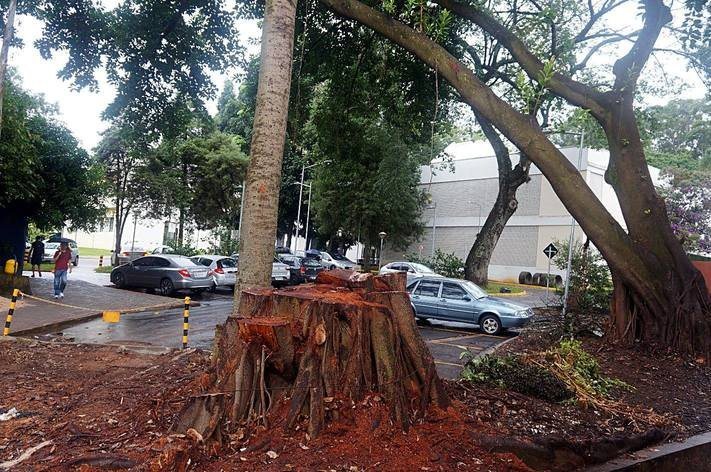
\includegraphics{figue}
\caption*{A figueira estável e mais desenvolvida foi removida, enquanto que a figueira mais inclinada (à direita da foto) foi mantida. Dois dias antes do depósito deste documento, havia profissionais realizando  levantamento topográfico na área. Faz pensar em qual seria o real critério do corte.}
\end{figure}
\end{landscape}

\newpage
\textbf{Compro Libras Arbóreas}
\begin{alltt}
          compro libras arbóreas
       2500lb            de madeira viva
            
               primeiro
               a do figo
               bem verdadeira
               
               restam na praça               
               seringueiras-falsas    uma fila
               e a viúva, abstrata,
              matemática, 
              à dentilhada valsa
              bem resistia

              \textit{F. elastica}
              \textit{ferrea} fosse
              menos brilharia
              a \textit{cementicia} viga

              latina ironia
              viga: \textit{Arbos},     \textit{concreta}  
\end{alltt}




\chapter{Resultados detalhados} \label{anresdet}
Os valores de ALC-$\mu_\kappa$ para todas as estratégias e conjuntos de dados são apresentados para cada algoritmo de aprendizado de máquina:
\begin{itemize}
   \item 5NN - tabelas \ref{stab5NNw0} e \ref{stab5NNw1};
   \item C4.5w - tabelas \ref{stabC4.520} e \ref{stabC4.521};
   \item NB - tabelas \ref{stabNB0} e \ref{stabNB1};
   \item SVM - tabelas \ref{stabSVM0} e \ref{stabSVM1};
   \item RFw - tabelas \ref{stabRFw0} e \ref{stabRFw1}; e,
   \item RoF - tabelas \ref{stabRoF0} e \ref{stabRoF1}.
\end{itemize}
%  \clearpage
\begin{landscape}
\begin{table}\centering\caption[Estratégias comparadas, conjuntos 1-45 com 5NN.]{Estratégias comparadas nos conjuntos de dados 1-45 com aprendiz 5NN. Medida: ALC-$\mu_\kappa$/$\sigma_\kappa$. \textit{Maior e menor média de cada linha estão em \textcolor{blue}{\textbf{negrito azul}} e \textcolor{red}{\textbf{negrito vermelho}} respectivamente. Maiores médias isoladas estão sublinhadas. Os melhores valores de desvio padrão estão em \textcolor{darkgreen}{verde}. Apenas negrito indica segundo melhor valor.}
}\label{stab5NNw0}
\scalebox{0.59}{	\begin{tabular}{lcccccccccccccc}\toprule\textbf{Conjunto de dados }& \textbf{ATUeuc} & \textbf{ATUman} & EERacc & EERent & HS & \textbf{HTUeuc} & \textbf{HTUman} & Mar & Rnd & \textbf{SGmulti} & TUeuc & TUman & DWeuc & DWman\\\midrule
	\input images/stab5NNw0
\bottomrule\end{tabular}}\end{table}
\begin{table}\centering\caption[Estratégias comparadas, conjuntos 46-90 com 5NN.]{Estratégias comparadas nos conjuntos de dados 46-90 com aprendiz 5NN. Medida: ALC-$\mu_\kappa$/$\sigma_\kappa$. \textit{Detalhes na Tabela \ref{stab5NNw0}.}
}\label{stab5NNw1}
\scalebox{0.605}{	\begin{tabular}{lcccccccccccccc}\toprule\textbf{Conjunto de dados }& \textbf{ATUeuc} & \textbf{ATUman} & EERacc & EERent & HS & \textbf{HTUeuc} & \textbf{HTUman} & Mar & Rnd & \textbf{SGmulti} & TUeuc & TUman & DWeuc & DWman\\\midrule
	\input images/stab5NNw1
\bottomrule\end{tabular}}\end{table}

\begin{table}\centering\caption[Estratégias comparadas, conjuntos 1-45 com C4.5w]{Estratégias comparadas nos conjuntos de dados 1-45 com aprendiz C4.5w. Medida: ALC-$\mu_\kappa$/$\sigma_\kappa$. \textit{Detalhes na Tabela \ref{stab5NNw0}.}
}\label{stabC4.520}
\scalebox{0.605}{	\begin{tabular}{lcccccccccccccc}\toprule\textbf{Conjunto de dados }& \textbf{ATUeuc} & \textbf{ATUman} & EERacc & EERent & HS & \textbf{HTUeuc} & \textbf{HTUman} & Mar & Rnd & \textbf{SGmulti} & TUeuc & TUman & DWeuc & DWman\\\midrule
	\input images/stabC4.520
\bottomrule\end{tabular}}\end{table}
\begin{table}\centering\caption[Estratégias comparadas, conjuntos 46-90 com C4.5w.]{Estratégias comparadas nos conjuntos de dados 46-90 com aprendiz C4.5w. Medida: ALC-$\mu_\kappa$/$\sigma_\kappa$. \textit{Detalhes na Tabela \ref{stab5NNw0}.}
}\label{stabC4.521}
\scalebox{0.605}{	\begin{tabular}{lcccccccccccccc}\toprule\textbf{Conjunto de dados }& \textbf{ATUeuc} & \textbf{ATUman} & EERacc & EERent & HS & \textbf{HTUeuc} & \textbf{HTUman} & Mar & Rnd & \textbf{SGmulti} & TUeuc & TUman & DWeuc & DWman\\\midrule
	\input images/stabC4.521
\bottomrule\end{tabular}}\end{table}

\begin{table}\centering\caption[Estratégias comparadas, conjuntos 1-45 com NB.]{Estratégias comparadas nos conjuntos de dados 1-45 com aprendiz NB. Medida: ALC-$\mu_\kappa$/$\sigma_\kappa$. \textit{Detalhes na Tabela \ref{stab5NNw0}.}
}\label{stabNB0}
\scalebox{0.605}{	\begin{tabular}{lcccccccccccccc}\toprule\textbf{Conjunto de dados }& \textbf{ATUeuc} & \textbf{ATUman} & EERacc & EERent & HS & \textbf{HTUeuc} & \textbf{HTUman} & Mar & Rnd & \textbf{SGmulti} & TUeuc & TUman & DWeuc & DWman\\\midrule
	\input images/stabNB0
\bottomrule\end{tabular}}\end{table}
\begin{table}\centering\caption[Estratégias comparadas, conjuntos 46-90 com NB.]{Estratégias comparadas nos conjuntos de dados 46-90 com aprendiz NB. Medida: ALC-$\mu_\kappa$/$\sigma_\kappa$. \textit{Detalhes na Tabela \ref{stab5NNw0}.}
}\label{stabNB1}
\scalebox{0.605}{	\begin{tabular}{lcccccccccccccc}\toprule\textbf{Conjunto de dados }& \textbf{ATUeuc} & \textbf{ATUman} & EERacc & EERent & HS & \textbf{HTUeuc} & \textbf{HTUman} & Mar & Rnd & \textbf{SGmulti} & TUeuc & TUman & DWeuc & DWman\\\midrule
	\input images/stabNB1
\bottomrule\end{tabular}}\end{table}

\begin{table}\centering\caption[Estratégias comparadas, conjuntos 1-45 com SVM.]{Estratégias comparadas nos conjuntos de dados 1-45 com aprendiz SVM. Medida: ALC-$\mu_\kappa$/$\sigma_\kappa$. \textit{Detalhes na Tabela \ref{stab5NNw0}.}
}\label{stabSVM0}
\scalebox{0.605}{	\begin{tabular}{lcccccccccccccc}\toprule\textbf{Conjunto de dados }& \textbf{ATUeuc} & \textbf{ATUman} & EERacc & EERent & HS & \textbf{HTUeuc} & \textbf{HTUman} & Mar & Rnd & \textbf{SGmulti} & TUeuc & TUman & DWeuc & DWman\\\midrule
	\input images/stabSVM0
\bottomrule\end{tabular}}\end{table}
\begin{table}\centering\caption[Estratégias comparadas, conjuntos 46-90 com SVM.]{Estratégias comparadas nos conjuntos de dados 46-90 com aprendiz SVM. Medida: ALC-$\mu_\kappa$/$\sigma_\kappa$. \textit{Detalhes na Tabela \ref{stab5NNw0}.}
}\label{stabSVM1}
\scalebox{0.58}{	\begin{tabular}{lcccccccccccccc}\toprule\textbf{Conjunto de dados }& \textbf{ATUeuc} & \textbf{ATUman} & EERacc & EERent & HS & \textbf{HTUeuc} & \textbf{HTUman} & Mar & Rnd & \textbf{SGmulti} & TUeuc & TUman & DWeuc & DWman\\\midrule
	\input images/stabSVM1
\bottomrule\end{tabular}}\end{table}

\begin{table}\centering\caption[Estratégias comparadas, conjuntos 1-45 com RFw.]{Estratégias comparadas nos conjuntos de dados 1-45 com aprendiz RFw. Medida: ALC-$\mu_\kappa$/$\sigma_\kappa$. \textit{Detalhes na Tabela \ref{stab5NNw0}.}
}\label{stabRFw0}
\scalebox{0.605}{	\begin{tabular}{lcccccccccccccc}\toprule\textbf{Conjunto de dados }& \textbf{ATUeuc} & \textbf{ATUman} & EERacc & EERent & HS & \textbf{HTUeuc} & \textbf{HTUman} & Mar & Rnd & \textbf{SGmulti} & TUeuc & TUman & DWeuc & DWman\\\midrule
	\input images/stabRFw0
\bottomrule\end{tabular}}\end{table}
\begin{table}\centering\caption[Estratégias comparadas, conjuntos 46-90 com RFw.]{Estratégias comparadas nos conjuntos de dados 46-90 com aprendiz RFw. Medida: ALC-$\mu_\kappa$/$\sigma_\kappa$. \textit{Detalhes na Tabela \ref{stab5NNw0}.}
}\label{stabRFw1}
\scalebox{0.605}{	\begin{tabular}{lcccccccccccccc}\toprule\textbf{Conjunto de dados }& \textbf{ATUeuc} & \textbf{ATUman} & EERacc & EERent & HS & \textbf{HTUeuc} & \textbf{HTUman} & Mar & Rnd & \textbf{SGmulti} & TUeuc & TUman & DWeuc & DWman\\\midrule
	\input images/stabRFw1
\bottomrule\end{tabular}}\end{table}

\begin{table}\centering\caption[Estratégias comparadas, conjuntos 1-45 com RoF.]{Estratégias comparadas nos conjuntos de dados 1-45 com aprendiz RoF. Medida: ALC-$\mu_\kappa$/$\sigma_\kappa$. \textit{Detalhes na Tabela \ref{stab5NNw0}.}
}\label{stabRoF0}
\scalebox{0.605}{	\begin{tabular}{lcccccccccccccc}\toprule\textbf{Conjunto de dados }& \textbf{ATUeuc} & \textbf{ATUman} & EERacc & EERent & HS & \textbf{HTUeuc} & \textbf{HTUman} & Mar & Rnd & \textbf{SGmulti} & TUeuc & TUman & DWeuc & DWman\\\midrule
	\input images/stabRoF0
\bottomrule\end{tabular}}\end{table}
\begin{table}\centering\caption[Estratégias comparadas, conjuntos 46-90 com RoF.]{Estratégias comparadas nos conjuntos de dados 46-90 com aprendiz RoF. Medida: ALC-$\mu_\kappa$/$\sigma_\kappa$. \textit{Detalhes na Tabela \ref{stab5NNw0}.}
}\label{stabRoF1}
\scalebox{0.605}{	\begin{tabular}{lcccccccccccccc}\toprule\textbf{Conjunto de dados }& \textbf{ATUeuc} & \textbf{ATUman} & EERacc & EERent & HS & \textbf{HTUeuc} & \textbf{HTUman} & Mar & Rnd & \textbf{SGmulti} & TUeuc & TUman & DWeuc & DWman\\\midrule
	\input images/stabRoF1
\bottomrule\end{tabular}}\end{table}


% \input images/stratstabALCKappaC4.52
% \input images/stratstabALCKappaNB
% \input images/stratstabALCKappaRFw
% \input images/stratstabALCKappaRoF
% \input images/stratstabALCKappaSVM

   \end{landscape}

\end{anexosenv}
\end{document}
